\documentclass[]{book}
\usepackage{lmodern}
\usepackage{amssymb,amsmath}
\usepackage{ifxetex,ifluatex}
\usepackage{fixltx2e} % provides \textsubscript
\ifnum 0\ifxetex 1\fi\ifluatex 1\fi=0 % if pdftex
  \usepackage[T1]{fontenc}
  \usepackage[utf8]{inputenc}
\else % if luatex or xelatex
  \ifxetex
    \usepackage{mathspec}
  \else
    \usepackage{fontspec}
  \fi
  \defaultfontfeatures{Ligatures=TeX,Scale=MatchLowercase}
\fi
% use upquote if available, for straight quotes in verbatim environments
\IfFileExists{upquote.sty}{\usepackage{upquote}}{}
% use microtype if available
\IfFileExists{microtype.sty}{%
\usepackage{microtype}
\UseMicrotypeSet[protrusion]{basicmath} % disable protrusion for tt fonts
}{}
\usepackage[margin=1in]{geometry}
\usepackage{hyperref}
\hypersetup{unicode=true,
            pdftitle={Dynamics of Complex Systems},
            pdfauthor={Fred Hasselman \& Maarten Wijnants},
            pdfborder={0 0 0},
            breaklinks=true}
\urlstyle{same}  % don't use monospace font for urls
\usepackage{natbib}
\bibliographystyle{apalike}
\usepackage{color}
\usepackage{fancyvrb}
\newcommand{\VerbBar}{|}
\newcommand{\VERB}{\Verb[commandchars=\\\{\}]}
\DefineVerbatimEnvironment{Highlighting}{Verbatim}{commandchars=\\\{\}}
% Add ',fontsize=\small' for more characters per line
\usepackage{framed}
\definecolor{shadecolor}{RGB}{248,248,248}
\newenvironment{Shaded}{\begin{snugshade}}{\end{snugshade}}
\newcommand{\KeywordTok}[1]{\textcolor[rgb]{0.13,0.29,0.53}{\textbf{{#1}}}}
\newcommand{\DataTypeTok}[1]{\textcolor[rgb]{0.13,0.29,0.53}{{#1}}}
\newcommand{\DecValTok}[1]{\textcolor[rgb]{0.00,0.00,0.81}{{#1}}}
\newcommand{\BaseNTok}[1]{\textcolor[rgb]{0.00,0.00,0.81}{{#1}}}
\newcommand{\FloatTok}[1]{\textcolor[rgb]{0.00,0.00,0.81}{{#1}}}
\newcommand{\ConstantTok}[1]{\textcolor[rgb]{0.00,0.00,0.00}{{#1}}}
\newcommand{\CharTok}[1]{\textcolor[rgb]{0.31,0.60,0.02}{{#1}}}
\newcommand{\SpecialCharTok}[1]{\textcolor[rgb]{0.00,0.00,0.00}{{#1}}}
\newcommand{\StringTok}[1]{\textcolor[rgb]{0.31,0.60,0.02}{{#1}}}
\newcommand{\VerbatimStringTok}[1]{\textcolor[rgb]{0.31,0.60,0.02}{{#1}}}
\newcommand{\SpecialStringTok}[1]{\textcolor[rgb]{0.31,0.60,0.02}{{#1}}}
\newcommand{\ImportTok}[1]{{#1}}
\newcommand{\CommentTok}[1]{\textcolor[rgb]{0.56,0.35,0.01}{\textit{{#1}}}}
\newcommand{\DocumentationTok}[1]{\textcolor[rgb]{0.56,0.35,0.01}{\textbf{\textit{{#1}}}}}
\newcommand{\AnnotationTok}[1]{\textcolor[rgb]{0.56,0.35,0.01}{\textbf{\textit{{#1}}}}}
\newcommand{\CommentVarTok}[1]{\textcolor[rgb]{0.56,0.35,0.01}{\textbf{\textit{{#1}}}}}
\newcommand{\OtherTok}[1]{\textcolor[rgb]{0.56,0.35,0.01}{{#1}}}
\newcommand{\FunctionTok}[1]{\textcolor[rgb]{0.00,0.00,0.00}{{#1}}}
\newcommand{\VariableTok}[1]{\textcolor[rgb]{0.00,0.00,0.00}{{#1}}}
\newcommand{\ControlFlowTok}[1]{\textcolor[rgb]{0.13,0.29,0.53}{\textbf{{#1}}}}
\newcommand{\OperatorTok}[1]{\textcolor[rgb]{0.81,0.36,0.00}{\textbf{{#1}}}}
\newcommand{\BuiltInTok}[1]{{#1}}
\newcommand{\ExtensionTok}[1]{{#1}}
\newcommand{\PreprocessorTok}[1]{\textcolor[rgb]{0.56,0.35,0.01}{\textit{{#1}}}}
\newcommand{\AttributeTok}[1]{\textcolor[rgb]{0.77,0.63,0.00}{{#1}}}
\newcommand{\RegionMarkerTok}[1]{{#1}}
\newcommand{\InformationTok}[1]{\textcolor[rgb]{0.56,0.35,0.01}{\textbf{\textit{{#1}}}}}
\newcommand{\WarningTok}[1]{\textcolor[rgb]{0.56,0.35,0.01}{\textbf{\textit{{#1}}}}}
\newcommand{\AlertTok}[1]{\textcolor[rgb]{0.94,0.16,0.16}{{#1}}}
\newcommand{\ErrorTok}[1]{\textcolor[rgb]{0.64,0.00,0.00}{\textbf{{#1}}}}
\newcommand{\NormalTok}[1]{{#1}}
\usepackage{longtable,booktabs}
\usepackage{graphicx,grffile}
\makeatletter
\def\maxwidth{\ifdim\Gin@nat@width>\linewidth\linewidth\else\Gin@nat@width\fi}
\def\maxheight{\ifdim\Gin@nat@height>\textheight\textheight\else\Gin@nat@height\fi}
\makeatother
% Scale images if necessary, so that they will not overflow the page
% margins by default, and it is still possible to overwrite the defaults
% using explicit options in \includegraphics[width, height, ...]{}
\setkeys{Gin}{width=\maxwidth,height=\maxheight,keepaspectratio}
\IfFileExists{parskip.sty}{%
\usepackage{parskip}
}{% else
\setlength{\parindent}{0pt}
\setlength{\parskip}{6pt plus 2pt minus 1pt}
}
\setlength{\emergencystretch}{3em}  % prevent overfull lines
\providecommand{\tightlist}{%
  \setlength{\itemsep}{0pt}\setlength{\parskip}{0pt}}
\setcounter{secnumdepth}{5}
% Redefines (sub)paragraphs to behave more like sections
\ifx\paragraph\undefined\else
\let\oldparagraph\paragraph
\renewcommand{\paragraph}[1]{\oldparagraph{#1}\mbox{}}
\fi
\ifx\subparagraph\undefined\else
\let\oldsubparagraph\subparagraph
\renewcommand{\subparagraph}[1]{\oldsubparagraph{#1}\mbox{}}
\fi

%%% Use protect on footnotes to avoid problems with footnotes in titles
\let\rmarkdownfootnote\footnote%
\def\footnote{\protect\rmarkdownfootnote}

%%% Change title format to be more compact
\usepackage{titling}

% Create subtitle command for use in maketitle
\newcommand{\subtitle}[1]{
  \posttitle{
    \begin{center}\large#1\end{center}
    }
}

\setlength{\droptitle}{-2em}
  \title{Dynamics of Complex Systems}
  \pretitle{\vspace{\droptitle}\centering\huge}
  \posttitle{\par}
  \author{Fred Hasselman \& Maarten Wijnants}
  \preauthor{\centering\large\emph}
  \postauthor{\par}
  \predate{\centering\large\emph}
  \postdate{\par}
  \date{2016-12-13}

\usepackage{booktabs}
\usepackage{longtable}
\usepackage{framed,color}
\definecolor{shadecolor}{RGB}{248,248,248}
\usepackage{natbib}
\usepackage[english]{babel}
\usepackage{amsmath,amsfonts,amssymb}
\usepackage{graphicx,xcolor}
\bibpunct{(}{)}{;}{a}{,}{,}
\usepackage{parskip}
\usepackage[margin=10pt,font=small]{caption}
\usepackage{placeins}
\usepackage{xcolor}
\usepackage{adjustbox}
\usepackage{float}
\usepackage{enumerate}
\usepackage{eso-pic}
\usepackage{everyshi}
\usepackage{bibentry}
\usepackage{changepage}
\usepackage{fontspec}

\DeclareGraphicsExtensions{.pdf,.png,.eps}

  \renewenvironment{quote}{%
  \par \small \medskip \block
  \leftskip=4em \rightskip=4em%
  \noindent \ignorespaces}{%
  \par \medskip
  }
 
\newcommand{\stitle}{Dynamics of Complex Systems}

% Headers
\usepackage{fancyhdr}
\pagestyle{fancy}
\fancyhf{}
\fancyhead[LE]{\nouppercase{\rightmark}}
\fancyhead[RO]{\textsc{\stitle}}
\fancyfoot[LE,RO]{\thepage}
\fancyheadoffset[RE,LO]{\textwidth}

% Create some reference defaults 
\captionsetup[figure]{labelfont=bf,labelsep=endash}
\captionsetup[table]{textfont=it,labelsep=newline}
\renewcommand{\thefigure}{\textbf{\arabic{chapter}.\arabic{figure}}}
\renewcommand{\thetable}{\textbf{\arabic{chapter}.\arabic{table}}}
%\renewcommand{\thechapter}{\textsc}

\let\stdsection\section
\renewcommand\section{\newpage\stdsection}

\setmainfont{Calibri}
\newfontface\itGS{Gill Sans Light Italic}
\newfontface\bfGS{Gill Sans SemiBold}
\newfontfamily\block{Gill Sans Light}

\ifxetex
  \usepackage{letltxmacro}
  \setlength{\XeTeXLinkMargin}{1pt}
  \LetLtxMacro\SavedIncludeGraphics\includegraphics
  \def\includegraphics#1#{% #1 catches optional stuff (star/opt. arg.)
    \IncludeGraphicsAux{#1}%
  }%
  \newcommand*{\IncludeGraphicsAux}[2]{%
    \XeTeXLinkBox{%
      \SavedIncludeGraphics#1{#2}%
    }%
  }%
\fi

\setkeys{Gin}{width=\linewidth}

\newenvironment{rmdblock}[1]
  {\begin{shaded*}
  \begin{itemize}
  \renewcommand{\labelitemi}{
    \raisebox{-.7\height}[0pt][0pt]{
      {\setkeys{Gin}{width=3em,keepaspectratio}\includegraphics{images/#1}}
    }
  }
  \item
  }
  {
  \end{itemize}
  \end{shaded*}
  }
\newenvironment{rmdnote}
  {\begin{rmdblock}{note}}
  {\end{rmdblock}}
\newenvironment{rmdselfThink}
  {\begin{rmdblock}{selfThink}}
  {\end{rmdblock}}
\newenvironment{rmdimportant}
  {\begin{rmdblock}{important}}
  {\end{rmdblock}}
\newenvironment{rmdkennen}
  {\begin{rmdblock}{kennen}}
  {\end{rmdblock}}
\newenvironment{rmdentertain}
  {\begin{rmdblock}{entertain}}
  {\end{rmdblock}}
\newenvironment{rmdfilo}
  {\begin{rmdblock}{Filosoof_150px}}
  {\end{rmdblock}}
\newenvironment{rmdempi}
  {\begin{rmdblock}{Empirist_150px}}
  {\end{rmdblock}}
\newenvironment{rmdscip}
  {\begin{rmdblock}{Sci-Pract_150px}}
  {\end{rmdblock}}

\let\BeginKnitrBlock\begin \let\EndKnitrBlock\end
\begin{document}
\maketitle

{
\setcounter{tocdepth}{1}
\tableofcontents
}
\chapter{\texorpdfstring{\textbf{Course
guide}}{Course guide}}\label{course-guide}

This course discusses research methods and analysis techniques that
allow for the study of human behaviour from a complex systems
perspective. Complexity research transcends the boundaries the classical
scientific disciplines in terms of explanatory goals
(e.g.~causal-mechanistic) and is a hot topic in physics, mathematics,
biology, economy and psychology.

The main focus in the cognitive behavioural sciences is a description
and explanation of behaviour based on interaction dominant dynamics:
Many processes interact on many different (temporal and spatial) scales
and observable behaviour emerges out of those interactions through a
process of self-organization or soft-assembly. Contrary to what the term
might suggest, complexity research is often about finding simple models
that are able to simulate a wide range of complex behaviour.

This approach differs fundamentally from the more classical approaches
where behaviour is caused by a system of many hidden (cognitive)
components which interact in sequence as in a machine (component
dominant dynamics). The most important difference is how `change', and
hence the time-evolution of a system, is studied.

The main focus of the course will be `hands-on' data-analysis in
\texttt{R}, or, in \texttt{Matlab} if student is already familiar with
the scritping language.

Topics include: Analysis of fractal geometry (i.e.~pink noise) in time
series (Standardized Dispersion Analysis, Power Spectral Density
Analysis, Detrended Fluctuation Analysis); Nonlinear and chaotic time
series analysis (Phase Space Reconstruction, (Cross) Recurrence
Quantification Analysis, Entropy Estimation); Growth Curve models;
Potential Theory; and Catastrophe Theory (Cusp model), Complex Network
Analysis.

\section{Learning objectives}\label{learning-objectives}

Students who followed this course will be able to critically evaluate
whether their scientific inquiries can benefit from adopting theories,
models, methods and analyses that were developed to study the dynamics
of complex systems. The student will be able to understand in more
detail the basics of formal theory evaluation, and be able to recognize,
interpret and deduce theoretical accounts of human behaviour that are
based on component-dominant versus interaction-dominant ontology.

Students will be able to use the basic mathematical models and analyses
that allow study of complex interaction-dominant behaviour. Students who
finish the course will be able to conduct analyses in \texttt{Excel},
\texttt{SPSS}, and \texttt{R} or \texttt{Matlab} and interpret the
results from basic (non-)linear time series methods. At the end of this
course, students have reached a level of understanding that allows them
to find relevant scientific sources and understand and follow up on new
developments in the complex systems approach to behavioural science.

\subsection*{Goals Summary}\label{goals-summary}
\addcontentsline{toc}{subsection}{Goals Summary}

\begin{itemize}
\tightlist
\item
  Read and understand papers that use a complex systems approach to
  study human behaviour.
\item
  Simulate the basic dynamical models.
\item
  Perform the basic analyses.
\end{itemize}

\section{Teaching methods}\label{teaching-methods}

Each meeting starts with a \emph{lecture session} addressing the
mathematical background and practical application of a particular aspect
of a model, or analysis technique. During the \emph{assignment session},
students will get hands-on experience with applying the models or
analysis techniques discussed during the lecture session by completing
assignments provided on blackboard for each session.

\subsection*{Preparation}\label{preparation}
\addcontentsline{toc}{subsection}{Preparation}

To prepare for each lecture students read a contemporary research paper
or watch a videolecture (e.g., \href{http://www.ted.com}{TED}) featuring
complexity theory and its application on a topic in behavioural science
that will be discussed in the subsequent lecture. Students are required
to formulate questions about each paper, and to initiate a discussion
with their fellow-students on Blackboard.

Before each lecture, students should:

\begin{itemize}
\tightlist
\item
  Read (parts of) a scientific article, or watch a videolecture
  featuring a complex systems perspective and/or methodology.
\item
  Ask (or answer) a question about what they have read / seen in the
  appropriate discussion forum on Blackboard.

  \begin{itemize}
  \tightlist
  \item
    The answers students provide will be discussed during the lecture.
  \end{itemize}
\end{itemize}

\section{Literature}\label{literature}

The following is part of the literature for this course:

\begin{itemize}
\tightlist
\item
  Lecture slides.
\item
  Articles and book chapters listed in the \texttt{Literature} folder on
  Blackboard for each session.
\item
  In addition, at the secretariat of PWO (5th floor, Spinoza building)
  selected chapters from the book ``Dynamical Psychology'' by Jay
  Friedenberg are available. It is not necessary to own the book to
  complete this course, but if you can find a copy, it may help to
  structure all the information provided during the course.
\end{itemize}

\emph{Note:} The literature for each session on Blackboard is provided
for reference, to fascilitate looking up a topic when it is needed to
complete the weekly assignments or the take-home exam.

\section{Schedule}\label{schedule}

The dates and locations can be found below. All lectures are on Tuesday
from \texttt{10.45} to \texttt{12.30}. The practical sessions take place
on Wednesday from \texttt{15.45} to \texttt{17.30}.

\begin{table}

\caption{\label{tab:setup2}Times and Places 2016-2017}
\centering
\begin{tabular}[t]{rlrllll}
\toprule
Lecture & Topic & Week & Day & Date & Activity type & Location\\
\midrule
1 & Introduction to Complexity Science & 46 & Tue & 2016-11-08 & Lecture & SP A -1.59\\
1 & Mathematics of Change I & 46 & Wed & 2016-11-09 & Lab course & SP A -1.55.A/B\\
2 & Multivariate Systems & 47 & Tue & 2016-11-15 & Lecture & SP A -1.59\\
2 & Mathematics of Change II & 47 & Wed & 2016-11-16 & Lab course & SP A -1.55.A/B\\
3 & Additive vs. Multiplicative Interactions & 48 & Tue & 2016-11-22 & Lecture & SP A -1.59\\
\addlinespace
3 & Basic Timeseries Analysis & 48 & Wed & 2016-11-23 & Lab course & SP A -1.55.A/B\\
4 & Fractal Geometry in Timeseries & 49 & Tue & 2016-12-29 & Lecture & SP A -1.59\\
4 & Fluctuation and Disperion analyses I & 49 & Wed & 2016-12-30 & Lab course & SP A -1.55.A/B\\
5 & Multi-Fractal Geometry in Timeseries & 50 & Tue & 2016-12-06 & Lecture & SP A -1.59\\
5 & Fluctuation and Disperion analyses II & 50 & Wed & 2016-12-07 & Lab course & SP A -1.55.A/B\\
\addlinespace
6 & Quantifying Continuous Dynamics & 51 & Tue & 2016-12-13 & Lecture & SP A -1.59\\
6 & Recurrence Quantification Analysis (RQA) & 51 & Wed & 2016-12-14 & Lab course & SP A -1.55.A/B\\
7 & Quantifying Categorical and Interaction Dynamics & 1 & Tue & 2016-01-20 & Lecture & SP A -1.59\\
7 & Categorical and Cross-Recurrence Quantification Analaysis (CRQA) & 1 & Wed & 2016-01-21 & Lab course & SP A -1.55.A/B\\
8 & Potential Theory and Catastrophe Theory & 2 & Tue & 2017-01-10 & Lecture & SP A -1.59\\
\addlinespace
8 & The Cusp Model & 2 & Wed & 2017-01-11 & Lab course & SP A -1.55.A/B\\
9 & Complex Networks & 3 & Tue & 2017-01-17 & Lecture & SP A -1.59\\
9 & Q\&A session & 3 & Wed & 2017-01-21 & Lab course & TvA 8.00.14\\
\bottomrule
\end{tabular}
\end{table}

\section{Examination}\label{examination}

The evaluation of achievement of study goals takes two forms:

\begin{itemize}
\tightlist
\item
  \textbf{Participation} - The ability to formulate a question about an
  advanced topic is a first step towards understanding, answering a
  question that was posted by a peer is a second step. Questions and
  answers will not be graded, there will be a check to see if a student
  participated in all sessions.
\item
  \textbf{Final Assignment} - This take-home assignment will be provided
  at the end of the course. It will consist of a series of practical
  assignments and at least one essay question to test theoretical
  knowledge. The submission deadline is two weeks after the last
  lecture.
\end{itemize}

\subsection*{Grading}\label{grading}
\addcontentsline{toc}{subsection}{Grading}

The take home exam will be graded as a regular exam. A student passes
the course if the exam grade is higher than 5.5 AND if the student
participated in the discussion on Blackboard each session.

\subsection*{Submitting the assignment}\label{submitting-the-assignment}
\addcontentsline{toc}{subsection}{Submitting the assignment}

The take-home exam must be submitted by sending them by email to both
\texttt{f.hasselman@pwo.ru.nl} AND \texttt{m.wijnants@pwo.ru.nl} no
later than \textbf{February 1st}.

\section{\texorpdfstring{We use \texttt{R}!}{We use R!}}\label{we-use-r}

This text was transformed to \texttt{HTML}, \texttt{PDF} en
\texttt{ePUB} using \texttt{bookdown}\citep{R-bookdown} in
\href{https://www.rstudio.com}{\textbf{RStudio}}, the graphical user
interface of the statistical language
\href{https://www.r-project.org}{\textbf{R}} \citep{R-base}.
\texttt{bookdown} makes use of the \texttt{R} version of
\href{https://en.wikipedia.org/wiki/Markdown}{markdown} called
\href{http://rmarkdown.rstudio.com}{Rmarkdown} \citep{R-rmarkdown},
together with \href{http://yihui.name/knitr/}{knitr} \citep{R-knitr} and
\href{http://pandoc.org}{pandoc}.

We'll use some web applications made in
\href{http://shiny.rstudio.com}{Shiny} \citep{R-shiny}

Other \texttt{R} packages used are: \texttt{DT} \citep{R-DT},
\texttt{htmlTable} \citep{R-htmlTable}, \texttt{plyr} \citep{R-plyr},
\texttt{dplyr} \citep{R-dplyr},\texttt{tidyr} \citep{R-tidyr},
\texttt{png} \citep{R-png}, \texttt{rio} \citep{R-rio}.

\part{Assignments}\label{part-assignments}

\chapter*{\texorpdfstring{\textbf{How to \ldots{}
}}{How to \ldots{} }}\label{how-to}
\addcontentsline{toc}{chapter}{\textbf{How to \ldots{} }}

These assignments were designed to prepare you for ``real world''
modelling and data analysis problems. That is, after completing the
assignments you should be able to decide whether the phenomenon you
study could benefit from a complex systems approach and which type of
analyses would be a good place to start. The models and techniques
discussed here are \textbf{not} a definite collection of available
techniques, this is really just the tip of the iceberg.

\subsection*{General Guidelines}\label{general-guidelines}
\addcontentsline{toc}{subsection}{General Guidelines}

\begin{itemize}
\tightlist
\item
  Read the instructions carefully.
\item
  Do not skip any of the steps.
\item
  Do not copy-paste from the assignment text into a spreadsheet or
  syntax editor (except for text in \texttt{code\ blocks}).
\item
  Study the solutions and lecture notes.
\end{itemize}

\subsection*{Files on GitHub}\label{files-on-github}
\addcontentsline{toc}{subsection}{Files on GitHub}

All the files (data, scripts, the files that generated this document)
are in a repository on
\href{https://github.com/FredHasselman/DCS}{Github}. Github keeps track
of all the different versions of the files in a repository.

\begin{itemize}
\tightlist
\item
  If you want to download a file that is basically a text file (e.g.~and
  \texttt{R} script), find a button named \texttt{raw}, then copy the
  text in your browser, or save as a text file.
\item
  For non-text files, a \texttt{download} button will be present
  somewhere on the page.
\end{itemize}

\chapter{\texorpdfstring{\textbf{Mathematics of Change
I}}{Mathematics of Change I}}\label{moc1ass}

In this assignment you will build two (relatively) simple
one-dimensional maps. We start with the \emph{Linear Map} and then
proceed to the slightly more complicated \emph{Logistic Map} (aka
\emph{Quadratic map}). You can use your favourite spreadsheet software
(e.g., Excel, Numbers, GoogleSheets).

\BeginKnitrBlock{rmdimportant}
If you are experienced in \texttt{R} or \texttt{Matlab} you can try to
code the models using the hints in section \ref{moc1R}.

Besure to check \protect\hyperlink{moc1Rsol}{the solutions of the
assigment} which provide examples of different ways to visualize the
time series in \texttt{R}
\EndKnitrBlock{rmdimportant}

\section{The Linear Map}\label{the-linear-map}

Equation \eqref{eq:linmap} is the ordinary difference equation (ODE)
discussed in the lecture (see lecture notes \ref{Lecture-1}) is called
the \emph{Linear Map}:

\begin{equation}
Y_{t+1} = Y_{t=0} + r*Y_t
\label{eq:linmap}
\end{equation}

In these excersises you will simulate \emph{time series} produced by the
change process in equation \ref@(eq:linmap) for different parameter
settings of the growth-rate parameter \(r\) (the \emph{control
parameter}) and the initial conditions \(Y_0\). This is different from a
statistical analysis in which parameters are estimated from a data set.
The goal of the assignments is to get a feeling for what a dynamical
model is, and how it is different from a linear statistical regression
model like GLM.

\subsection{The Linear Map in a
Spreadsheet}\label{the-linear-map-in-a-spreadsheet}

\BeginKnitrBlock{rmdimportant}
Before you begin, be sure to check the following settings:

\begin{itemize}
\tightlist
\item
  Open a Microsoft Excel worksheet, a
  \href{https://www.google.com/docs/about/}{Google sheet}, or other
  spreadsheet.
\item
  Check whether the spreadsheet uses a `decimal-comma' (\(0,05\)) or
  `decimal-point' (\(0.05\)) notation.

  \begin{itemize}
  \tightlist
  \item
    The numbers given in the assignments of this course all use a
    `decimal-point' notation.
  \end{itemize}
\item
  Check if the \texttt{\$} symbol fixes rows and columns when it used in
  a formula in your preferred spreadsheet program.

  \begin{itemize}
  \tightlist
  \item
    This is the default setting in Microsoft Excel and Google. If you
    use one of those programs you are all set, otherwise you will have
    to replace the \texttt{\$} used in the assignments with the one used
    by your software.

    \EndKnitrBlock{rmdimportant}
  \end{itemize}
\item
  Type \texttt{r} in cell \texttt{A5}. This is the \emph{control
  parameter}. It receives the value \(1.08\) in cell\texttt{B5}.
\item
  Type \(Y_0\) in cell \texttt{A6}. This is the \emph{initial value}. It
  receives the value \(0.1\) in cell \texttt{B6}.\\
\item
  Use the output level (\(Y_t\)) of every step as the input to calculate
  the next level (\(Y_{t+1}\)).

  \begin{itemize}
  \tightlist
  \item
    Rows in the spreadsheet will represent the values of the process at
    different moments in time.
  \end{itemize}
\item
  Put the initial value (\(Y_0\)) in cell \texttt{A10}. This cell marks
  time \(t=0\).

  \begin{itemize}
  \tightlist
  \item
    To get it right, type: \texttt{=\$B\$6}. The \texttt{=} means that
    (in principle) there is a `calculation' going on (a function is
    applied). The \texttt{\$} determines that column (\texttt{\$B}) as
    well as the row (\texttt{\$6}) keep the same value (i.e., constant)
    for each time step.
  \end{itemize}
\item
  Enter the \textbf{Linear Map} as a function in each cell. Type
  \texttt{=\$B\$5*A10} in cell \texttt{A11}.

  \begin{itemize}
  \tightlist
  \item
    This means that the value of cell \texttt{A11} (i.e. \(Y_{t=1}\))
    will be calculated by multiplying the value of cell \texttt{B5}
    (parameter \texttt{r}) with the value of cell \texttt{A10} (previous
    value, here: \(Y_{t=0}\)). If everything is all right, cell
    \texttt{A11} now shows the value \(0.108\).
  \end{itemize}
\item
  Repeat this step for cell \texttt{A12}.

  \begin{itemize}
  \tightlist
  \item
    Remember what it is you are doing! You are calculating \(Y_{t=2}\)
    now (i.e.~the next step), which is determined by \(Y_{t=1}\) (i.e.,
    the previous step) and the parameter \texttt{r}.
  \end{itemize}
\item
  Now repeat this simple iterative step for \texttt{100} further steps.
  Instead of typing everything over and over again, copy-paste the whole
  thing.Most spreadsheet programs will automatically adjust the formula
  by advancing each row or column number that aren't fixed by
  \texttt{\$}.

  \begin{itemize}
  \tightlist
  \item
    Copy cell \texttt{A12} all the way from \texttt{A13} to
    \texttt{A110} (keep the \texttt{SHIFT} button pressed to select all
    cells).
  \end{itemize}
\end{itemize}

\texttt{You\ have\ just\ simulated\ a\ time\ series\ based\ on\ a\ theoretical\ change\ process!}

\subsection{Visualizing the time
series}\label{visualizing-the-time-series}

\begin{enumerate}
\item
  Select cells \texttt{A10} to \texttt{A110} Create a line graph
  (\texttt{Insert}, 2D-line, Scatter). This will show you the graph.
  (There are other ways to do this, by the way, which work just as
  well.) You can play with the setting to make the best suitable view,
  like rescaling the axes.
\item
  If you change the values in cells B5 and B6 you will see an immediate
  change in the graph. To study model behaviour, try the following
  growth parameters:

  \begin{itemize}
  \tightlist
  \item
    \(a = -1.08\)
  \item
    \(a = 1,08\)
  \item
    \(a = 1\)
  \item
    \(a = -1\)
  \end{itemize}
\item
  Change the initial value \(Y_0\) in cell \texttt{B6} to \(10\).
  Subsequently give the growth parameter in cell \texttt{B5} the
  following values \(0.95\) and \(-0.95\).
\end{enumerate}

\section{The Logistic Map in a
spreadsheet}\label{the-logistic-map-in-a-spreadsheet}

The Logistic Map takes the following functional form:

\begin{equation}
Y_{t+1} = r*Y_t*(1-Y_t)
\label{eq:logmap}
\end{equation}

To get started, copy the spreadsheet from the previous assignment to a
new sheet. The parameters are the same as for the Linear Map, there has
to be an initial value \(Y_{t=0}\) (no longer explicit as a constant in
equation \eqref{eq:logmap}) and the control parameter \(r\). What will
have to change is

\begin{itemize}
\tightlist
\item
  Start with the following values for control parameter \(r\):

  \begin{itemize}
  \tightlist
  \item
    \(r = 1.9\)
  \item
    \(Y_0 = 0.01\) (in \texttt{A6}).
  \end{itemize}
\item
  Take good notice of what is constant (parameter \(r\)), so for which
  the \texttt{\$} must be used, and what must change on every iterative
  step (variable \(Y_t\)).
\end{itemize}

\subsection{Visualizing the time series and explore its
behaviour}\label{visualizing-the-time-series-and-explore-its-behaviour}

\begin{itemize}
\tightlist
\item
  Create the time series graphs as for the Linear Map.
\end{itemize}

To study the behavior of the Logistic Map you can start playing around
with the values for the parameters and the initial values in cells
\texttt{B5} and \texttt{B6}.

\begin{itemize}
\tightlist
\item
  Be sure to try the following settings for \(r\):

  \begin{itemize}
  \tightlist
  \item
    \(r = 0.9\)
  \item
    \(r = 1.9\)
  \item
    \(r = 2.9\)
  \item
    \(r = 3.3\)
  \item
    \(r = 3.52\)
  \item
    \(r = 3.9\)
  \end{itemize}
\item
  Set \(r\) at \(4.0\):

  \begin{itemize}
  \tightlist
  \item
    Repeat the iterative process from \texttt{A10} to \texttt{A310} (300
    steps)
  \item
    Now copy \texttt{A10:A310} to \texttt{B9:B309} (i.e., move it one
    cell to the right, and one cell up)
  \item
    Select both columns (\texttt{A10} to \texttt{B309}!) and make a
    scatter-plot
  \end{itemize}
\end{itemize}

\hypertarget{the-return-plot}{\subsection{The return
plot}\label{the-return-plot}}

The plot you just produced is a so called \textbf{return plot}, in which
you have plotted \(Y_{t+1}\) against \(Y_t\).

\begin{itemize}
\tightlist
\item
  Can you explain the pattern you see (a `parabola') by looking closely
  at the functional form of the Logistic Map? (hint: it's also called
  \textbf{Quadratic Map})

  \begin{itemize}
  \tightlist
  \item
    Look at what happens in the return plot when you change the value of
    the parameter \(r\) (in \texttt{A5}).
  \item
    What do you expect the return plot of the Linear Map will look like?
    Try it!
  \end{itemize}
\end{itemize}

The meaning and use of this plot was discussed in the next session

\section{\texorpdfstring{Using \texttt{R} or \texttt{Matlab} to do the
exercises.}{Using R or Matlab to do the exercises.}}\label{moc1R}

The best (and easiest) way to simulate these simple models is to create
a function which takes as input the parameters (\(Y_0\), \(r\)) and a
variable indicating the length of the time series.

For example for the Linear Map:

\begin{Shaded}
\begin{Highlighting}[]
\CommentTok{# In R}
\NormalTok{linearMap <-}\StringTok{ }\NormalTok{function(}\DataTypeTok{Y0 =} \DecValTok{0}\NormalTok{, }\DataTypeTok{r =} \DecValTok{1}\NormalTok{, }\DataTypeTok{N =} \DecValTok{100}\NormalTok{)\{}
    
    \CommentTok{# Initialize Y as an NA vector of size N with as first entry Y0}
    \NormalTok{Y <-}\StringTok{ }\KeywordTok{c}\NormalTok{(Y0, }\KeywordTok{rep}\NormalTok{(}\OtherTok{NA}\NormalTok{,N}\DecValTok{-1}\NormalTok{))}
    
    \NormalTok{for(i in }\DecValTok{1}\NormalTok{:N)\{}
        
    \NormalTok{Y[i}\DecValTok{+1}\NormalTok{] <-}\StringTok{ }\CommentTok{# Implement the function here}
\StringTok{        }
\StringTok{    }\NormalTok{\}}
    
    \KeywordTok{return}\NormalTok{(Y)}
\NormalTok{\}}


\CommentTok{# In Matlab}
\NormalTok{function }\KeywordTok{linearMap}\NormalTok{(Y0,r,N)}
 \CommentTok{# Implement the function here}
\NormalTok{end}
\end{Highlighting}
\end{Shaded}

Creating the time series graphs and the return plot should be easy if
the function \texttt{linearMap} returns the time series. Both \texttt{R}
and \texttt{Matlab} have a \texttt{plot()} function you can
call.\footnote{Both \texttt{R} and \texttt{Matlab} have specialized
  objects to represent timeseries, and functions and packages for
  timeseries analysis. They are especially convenient for plotting time
  and date information on the X-axis. See Solutions:
  \protect\hyperlink{moc1Rsol}{Mathematics of Change I}}

\chapter{\texorpdfstring{\textbf{Mathematics of Change
II}}{Mathematics of Change II}}\label{moc2ass}

In this assignment we will build a more sophisticated growth modeland
look at its properties. The model will be the growth model by Van Geert
(1991 etc.) as discussed in the book chapter you read. If your are
experienced in \texttt{R} or \texttt{Matlab} you can try to code the
models following the hints in section \ref{moc1R}.

\subsection*{The growth model by Van Geert
(1991)}\label{the-growth-model-by-van-geert-1991}
\addcontentsline{toc}{subsection}{The growth model by Van Geert (1991)}

The growth model by Van Geert has the following form:

\begin{equation}
L_{t+1} = L_t * (1 + r - r * \frac{L_t}{K})
\label{eq:vanG}
\end{equation}

Note the similarities to Equation \eqref{eq:logmap}, the (stylized)
logistic map.

\section{The growth model in a
spreadsheet}\label{the-growth-model-in-a-spreadsheet}

\BeginKnitrBlock{rmdimportant}
Before you begin, be sure to check the following settings (same as first
asignment):

\begin{itemize}
\tightlist
\item
  Open a Microsoft Excel worksheet or a
  \href{https://www.google.com/docs/about/}{Google sheet}
\item
  Check whether the spreadsheet uses a `decimal-comma' (\(0,05\)) or
  `decimal-point' (\(0.05\)) notation.

  \begin{itemize}
  \tightlist
  \item
    The numbers given in the assignments of this course all use a
    `decimal-point' notation.
  \end{itemize}
\item
  Check if the \texttt{\$} symbol fixes rows and columns when it used in
  a formula in your preferred spreadsheet program.

  \begin{itemize}
  \tightlist
  \item
    This is the default setting in Microsoft Excel and Google Sheets. If
    you use one of those programs you are all set.

    \EndKnitrBlock{rmdimportant}
  \end{itemize}
\end{itemize}

To build it repeat some of the steps you performed in assignment
\ref{moc1ass} on a new worksheet.

\begin{itemize}
\tightlist
\item
  Define the appropriate constants (\(r\) in \texttt{A5}, \(L_0\) in
  \texttt{A6}) and prepare the necessary things you need for building an
  iterative process.
\item
  In particular, add the other parameter that appears in Van Geert???s
  model:

  \begin{itemize}
  \tightlist
  \item
    Type \(K\) in cell \texttt{A7}. This is the \emph{carrying
    capacity}. It receives the value \(1\) in cell \texttt{B7}.
  \end{itemize}
\item
  Start with the following values:

  \begin{itemize}
  \tightlist
  \item
    \(r = 1.2\)
  \item
    \(L_0 = 0.01\)
  \end{itemize}
\end{itemize}

Take good notice of what is constant (parameters \(r\) and \(K\)), for
which the \texttt{\$} must be used, and what must change on every
iterative step (variable \(L_t\)). Take about \(100\) steps.

\begin{itemize}
\tightlist
\item
  Create the graphs
\item
  You can start playing with the values for the parameters and the
  initial values in cells \texttt{B5}, \texttt{B6} and \texttt{B7}. To
  study this model???s behavior, be sure to try the following growth
  parameters:

  \begin{itemize}
  \tightlist
  \item
    \(r = 1.2\)
  \item
    \(r = 2.2\)
  \item
    \(r = 2.5\)
  \item
    \(r = 2.7\)
  \item
    \(r = 2.9\)
  \end{itemize}
\item
  For the carrying capacity \(K\) (cell \texttt{B7}) you can try the
  following values:

  \begin{itemize}
  \tightlist
  \item
    \(K = 1.5\)
  \item
    \(K = 0.5\). (Leave \(r = 2.9\). Mind the value on the vertical
    axis!)
  \end{itemize}
\item
  Changes in the values of \(K\) have an effect on the height of the
  graph. The pattern itself also changes a bit. Can you explain why this
  is so?
\end{itemize}

\section{Conditional growth: Jumps and
Stages}\label{conditional-growth-jumps-and-stages}

\subsection*{Auto-conditional jumps}\label{auto-conditional-jumps}
\addcontentsline{toc}{subsection}{Auto-conditional jumps}

Suppose we want to model that the growth rate \(r\) increases after a
certain amount has been learned. In general, this is a very common
phenomenon, for instance: when becoming proficient at a skill, growth
(in proficiency) is at first slow, but then all of a sudden there can be
a jump to the appropriate (and sustained) level of proficiency.

\begin{itemize}
\tightlist
\item
  Take the model you just built as a starting point with \(r = 0.1\)
  (\texttt{B5})

  \begin{itemize}
  \tightlist
  \item
    Type \(0.5\) in \texttt{C5}. This will be the new parameter value
    for \(r\).
  \item
    Build your new model in column \texttt{B} (leave the original in
    \texttt{A}).
  \end{itemize}
\item
  Suppose we want our parameter to change when a growth level of \(0.2\)
  is reached. We???ll need an \texttt{IF} statement which looks
  something like this: \texttt{IF} \(L > 0.2\) then use the parameter
  value in \texttt{C5}, otherwise use the parameter value in
  \texttt{B5}.

  \begin{itemize}
  \tightlist
  \item
    Excel has a built in \texttt{IF} function (may be \texttt{ALS} in
    Dutch).
  \item
    In the first cell in which calculations should start, press \(=\)
    and then from the formula list choose the \texttt{IF} function, or
    just type it.
  \item
    Try to figure out what you have to do. In the Logical\_test box you
    should state something which expresses \(L > 0.2\).
  \item
    The other fields tell Excel what to do when this statement is
    \texttt{TRUE} (then use parameter value in \texttt{C5}) or when it
    is \texttt{FALSE} (then use paramter value in \texttt{B5}).
  \item
    \textbf{Note:} the word \emph{value} might be misleading; you can
    also input new statements.
  \end{itemize}
\item
  Make a graph in which the old and the new conditional models are
  represented by lines.

  \begin{itemize}
  \tightlist
  \item
    Try changing the value of \(r\) in \texttt{C5} into:
    \(1, 2, 2.8, 2.9, 3\).
  \end{itemize}
\end{itemize}

\subsection*{Auto-conditional stages}\label{auto-conditional-stages}
\addcontentsline{toc}{subsection}{Auto-conditional stages}

Another conditional change we might want to explore is that when a
certain growth level is reached the carrying capacity K increases,
reflecting that new resources have become available to support further
growth.

\begin{itemize}
\item
  Now we want \(K\) to change, so type \(1\) in \texttt{B7}, \(2\) in
  \texttt{C7}.
\item
  Build your model in column C. Follow the same steps as above, but now
  make sure that when \(L > 0.99\), \(K\) changes to the value in
  \texttt{C7}. Keep \(r = 0.2\) (\texttt{B5}).
\item
  If all goes well you should see two stages when you create a graph of
  the timeseries in column \texttt{C}. Change \(K\) in \texttt{C7} to
  other values.

  \begin{itemize}
  \tightlist
  \item
    Try to also change the growth rate r after reaching \(L > 0.99\) by
    referring to \texttt{C5}. Start with a value of \(0.3\) in
    \texttt{C5}. Set \(K\) in \texttt{C7} to \(2\) again.
  \item
    Also try \(1, 2.1, 2.5, 2.6, 3\).
  \end{itemize}
\end{itemize}

\subsection*{Connected growers}\label{connected-growers}
\addcontentsline{toc}{subsection}{Connected growers}

You can now easly model coupled growth processes, in which the values in
one series serve as the trigger for for parameter changes in the other
process. Try to recreate the Figure of the connected growers printed in
the chapter by Van Geert.

\subsubsection{Demonstrations of dynamic modeling using
spreadsheets}\label{demonstrations-of-dynamic-modeling-using-spreadsheets}

See the website by \href{http://www.paulvangeert.nl/research.htm}{Paul
Van Geert}, scroll down to see models of:

\begin{itemize}
\tightlist
\item
  Learning and Teaching
\item
  Behaviour Modification
\item
  Connected Growers
\item
  Interaction during Play
\end{itemize}

\section{Iterating 2D Maps and Flows}\label{iterating-2d-maps-and-flows}

In this assignment we will look at a 2D coupled dynamical system:
\textbf{the Predator-Prey model} (aka
\href{https://en.wikipedia.org/wiki/Lotka???Volterra_equations}{Lotka-Volterra
equations}). If your are experienced in \texttt{R} or \texttt{Matlab}
you can try to code the models following the instructions at the end of
this assignment.

\section{Predator-prey model}\label{predator-prey-model}

The dynamical system is given by the following set of first-order
differential equations, one represents changes in a population of
predators, (e.g., \textbf{F}oxes: \(f_F(R_t,F_t)\) ), the other
represents changes in a population of prey, (e.g., \textbf{R}abbits:
\(f_R(R_t,F_t)\) ).

\begin{align}
\frac{dR}{dt}&=(a-b*F)*R \\
\\
\frac{dF}{dt}&=(c*R-d)*F
\label{eq:lv}
\end{align}

This is not a \emph{difference} equation but a \emph{differential}
equation, which means building this system is not as straightforward as
was the case in the previous assignments. Simulation requires a
numerical method to `solve' this differential equation for time, which
means we need a method to approach, or estimate continuous time in
discrete time. Below you will receive a speed course in one of the
simplest numerical procedures for integrating differential equations,
the \href{https://en.wikipedia.org/wiki/Euler_method}{Euler method}.

\subsection{Euler Method}\label{euler-method}

A general differential equation is given by:

\begin{equation}
\frac{dx}{dt} = f(x)
\label{eq:diff}
\end{equation}

Read it as saying: ``\emph{a change in \(x\) over a change in time is a
function of \(x\) itself}''. This can be approximated by considering the
change to be over some constant, small time step \(\Delta\):

\begin{equation}
\frac{(x_{t+1} = x_t)}{\Delta} = f(x_t)
\label{eq:Euler}
\end{equation}

After rearranging the terms a more familiar form reveals itself:

\begin{align}
x_{t+1} &= x_t &= f(x_t) * \Delta \\
x_{t+1} &= f(x_t) * \Delta + x_t
\label{eq:Euler2}
\end{align}

This looks like an ordinary iterative process, \(\Delta\) the \emph{time
constant} determines the size of time step taken at every successive
iteration. For a 2D system with variables \textbf{R} and \textbf{F} on
would write:

\begin{align}
R_{t+1} &= f_R(R_t,Ft) * \Delta + R_t \\
F_{t+1} &= f_F(R_t,F_t) * \Delta + F_t
\label{eq:EulerRF}
\end{align}

\subsection{Coupled System in a
spreadsheet}\label{coupled-system-in-a-spreadsheet}

Implement the model in a spreadsheet by substituting \(f_R(R_t,Ft)\) and
\(f_F(R_t,F_t)\) by the differential equations for Foxes and Rabbits
given above.

\begin{itemize}
\tightlist
\item
  Start with \(a = d = 1\) and \(b = c = 2\) and the initial conditions
  \(R_0 = 0.1\) and \(F_0 = 0.1\). Use a time constant of \(0.01\) and
  make at least \(1000\) iterations.
\item
  Visualize the dynamics of the system by plotting:

  \begin{itemize}
  \tightlist
  \item
    \(F\) against \(R\) (i.e., the state space)
  \item
    \(R\) and \(F\) against time (i.e., the timeseries) in one plot.
  \end{itemize}
\item
  Starting from the initial predator and prey population represented by
  the point \((R, F) = (0.1, 0.1)\), how do the populations evolve over
  time?
\item
  Try to get a grip on the role of the time constant by increasing and
  decreasing it slightly (e.g. \(\Delta = 0.015\)) for fixed parameter
  values. (You might have to add some more iterations to complete the
  plot). What happens to the plot?

  \begin{itemize}
  \tightlist
  \item
    Hint: Remember that \(\Delta\) is not a fundamental part of the
    dynamics, but that it is only introduced by the numerical
    integration (i.e., the approximation) of the differential equation.
    It should not change the dynamics of the system, but it has an
    effect nonetheless.
  \end{itemize}
\end{itemize}

\protect\hyperlink{ppdsol}{\textbar{} jump to solution \textbar{}}

\section{The Competetive Lottka-Volterra
Equations}\label{the-competetive-lottka-volterra-equations}

The coupled predator-prey dynamics in the previous assignment are not a
very realistic model of an actual ecological system. Both equations are
exponential growth functions, but \textbf{R}abbits for example, also
have to eat! One way to increase realism is to consider coupled logistic
growth by introducing a carrying capacity.

\begin{itemize}
\tightlist
\item
  Follow the link to the
  \href{https://en.wikipedia.org/wiki/Competitive_Lotka???Volterra_equations}{Wiki
  page} and try to model the system!
\end{itemize}

\begin{quote}
This is what \emph{interaction dynamics} refers to, modeling mutual
dependiencies using the \texttt{if\ ...\ then} conditional rules isn't
really about interaction, or coupling between processes.
\end{quote}

\section{Predator-Prey (and other) dynamics as Agent Based
Models}\label{predator-prey-and-other-dynamics-as-agent-based-models}

Agent-Based models are an expansion of the idea of ``connected growers''
that includes a spatial location of the things that is subject to change
over time.

Have a look at some of the
\href{http://ccl.northwestern.edu/netlogo/}{NETlogo} demo's:

\begin{itemize}
\tightlist
\item
  \href{http://www.netlogoweb.org/launch\#http://www.netlogoweb.org/assets/modelslib/Sample\%20Models/Biology/Rabbits\%20Grass\%20Weeds.nlogo}{Rabbits
  Weeds Grass}
\item
  \href{http://www.netlogoweb.org/launch\#http://www.netlogoweb.org/assets/modelslib/Sample\%20Models/Biology/Wolf\%20Sheep\%20Predation.nlogo}{Wolf
  Sheep Grass}
\end{itemize}

\chapter{\texorpdfstring{\textbf{Basic Timeseries
Analysis}}{Basic Timeseries Analysis}}\label{basic-timeseries-analysis}

Most of the basic timeseries analyses can be performed in \texttt{SPSS},
because many of you will be familiar with the software we present the
first assignments mainly as \texttt{SPSS} instructions, but you can go
ahead an try your preferred environment for (statistical) computing.

\BeginKnitrBlock{rmdimportant}
See the comments about \protect\hyperlink{bTSAinR}{using \texttt{R} and
\texttt{Matlab}})
\EndKnitrBlock{rmdimportant}

\section{Time series analysis in SPSS (17 and
higher)}\label{time-series-analysis-in-spss-17-and-higher}

\hypertarget{bta}{\subsection{Nonlinear Growth curves in
SPSS}\label{bta}}

\begin{itemize}
\tightlist
\item
  Open the file
  \href{https://github.com/FredHasselman/DCS/blob/master/assignmentData/BasicTSA_nonlinreg/GrowthRegression.sav}{Growthregression.sav},
  it contains two variables: \texttt{Time} and \texttt{Y(t)}.
\end{itemize}

This is data from an iteration of the logistic growth differential
equation you are familiar with by now, but let's pretend it's data from
one subject measured on 100 occasions.

\begin{enumerate}
\def\labelenumi{\arabic{enumi}.}
\tightlist
\item
  Plot Y(t) against Time Recognize the shape?
\item
  To get the growth parameter we'll try to fit the solution of the
  logistic flow with SPSS nonlinear regression

  \begin{itemize}
  \tightlist
  \item
    Select nonlinear\ldots{} from the \texttt{Analysis}
    \textgreater{}\textgreater{} \texttt{Regression} menu.
  \item
    Here we can build the solution equation. We need three parameters:
    a. \textbf{Yzero}, the initial condition. b. \emph{K}, the carrying
    capacity. c. \emph{r}, the growth rate.
  \item
    Fill these in where it says \texttt{parameters} give all parameters
    a starting value of \(0.01\)
  \end{itemize}
\item
  Take a good look at the analytic solution of the (stilized) logistic
  flow:
\end{enumerate}

\[
Y(t)  =  \frac{K * Y_0}{Y_0 + \left(K-Y_{0}\right) * e^{(-K*r*t)} }
\]

Tr to build this equation, the function fo \(e\) is called \texttt{EXP}
in \texttt{SPSS} (\texttt{Function\ Group} \textgreater{}\textgreater{}
\texttt{Arithmetic}) Group terms by using parentheses as shown in the
equation.

\begin{enumerate}
\def\labelenumi{\arabic{enumi}.}
\setcounter{enumi}{4}
\item
  If you think you have built the model correctly, click on
  \texttt{Save} choose \texttt{predicted\ values}. Then paste your
  syntax and run it!

  \begin{itemize}
  \tightlist
  \item
    Check the estimated parameter values.
  \item
    Check \(R^2\)!!!
  \end{itemize}
\item
  Plot a line graph of both the original data and the predicted values.
  (Smile)
\item
  A polynomial fishing expedition:

  \begin{itemize}
  \item
    Create time-varying covariates of \(Y(t)\):

\begin{verbatim}
COMPUTE T1=Yt * Time.
COMPUTE T2=Yt * (Time ** 2). 
COMPUTE T3=Yt * (Time ** 3). 
COMPUTE T4=Yt * (Time ** 4). 
EXECUTE.
\end{verbatim}
  \item
    Use these variables as predictors of \(Y(t)\) in a regular linear
    regression analysis. This is called a \emph{polynomial regression}:
    Fitting combinations of curves of different shapes on the data.
  \item
    Before you run the analysis: Click \texttt{Save} Choose
    \texttt{Predicted\ Values:\ Unstandardized}
  \end{itemize}
\item
  Look at \(R^2\). This is also almost 1. Which model is better? Think
  about this: Based o the results o the linear regression what can yo
  tell about the \emph{growth rate}, the \emph{carrying capacity} or the
  \emph{initial condition}?
\item
  Create a line graph of \(Y(t)\), plot the predicted values of the
  nonlinear regression and the unstandardized predicted values of the
  linear polynomial regression against \texttt{time} in one figure.
\item
  Now you can see that the shape is approximated by the polynomials, but
  it is not quite the same. Is this really a model of a growth process
  as we could encounter it in nature?
\end{enumerate}

\protect\hyperlink{btasol}{\textbar{} jump to solution \textbar{}}

\hypertarget{pacf}{\subsection{Correlation functions and AR-MA
models}\label{pacf}}

\begin{enumerate}
\def\labelenumi{\arabic{enumi}.}
\item
  Download the file
  \href{https://github.com/FredHasselman/DCS/blob/master/assignmentData/BasicTSA_arma/series.sav}{\texttt{series.sav}}
  from blackboard. It contains three time series \texttt{TS\_1},
  \texttt{TS\_2} and \texttt{TS\_3}. As a first step look at the mean
  and the standard deviation (\texttt{Analyze}
  \textgreater{}\textgreater{} \texttt{Descriptives}). Suppose these
  were time series from three subjects in an experiment, what would you
  conclude based on the means and SD's?
\item
  Let's visualize these data. Go to \texttt{Forecasting}
  \textgreater{}\textgreater{} \texttt{Time\ Series}
  \textgreater{}\textgreater{} \texttt{Sequence\ Charts}. Check the box
  One chart per variable and move all the variables to Variables. Are
  they really the same?
\item
  Let's look at the \texttt{ACF} and \texttt{PCF}

  \begin{itemize}
  \tightlist
  \item
    Go to \texttt{Analyze} \textgreater{}\textgreater{}
    \texttt{Forecasting} \textgreater{}\textgreater{}
    \texttt{Autocorrelations}.
  \item
    Enter all the variables and make sure both \emph{Autocorrelations}
    (ACF) and \emph{Partial autocorrelations} (PACF) boxes are checked.
    Click \texttt{Options}, and change the
    \texttt{Maximum\ Number\ of\ Lags} to \texttt{30}.
  \item
    Use the table to characterize the time series:
  \end{itemize}
\end{enumerate}

\begin{longtable}[]{@{}ll@{}}
\toprule
\begin{minipage}[b]{0.28\columnwidth}\raggedright\strut
SHAPE\strut
\end{minipage} & \begin{minipage}[b]{0.66\columnwidth}\raggedright\strut
INDICATED MODEL\strut
\end{minipage}\tabularnewline
\midrule
\endhead
\begin{minipage}[t]{0.28\columnwidth}\raggedright\strut
Exponential, decaying to zero\strut
\end{minipage} & \begin{minipage}[t]{0.66\columnwidth}\raggedright\strut
Autoregressive model. Use the partial autocorrelation plot to identify
the order of the autoregressive model\strut
\end{minipage}\tabularnewline
\begin{minipage}[t]{0.28\columnwidth}\raggedright\strut
Alternating positive and negative, decaying to zero\strut
\end{minipage} & \begin{minipage}[t]{0.66\columnwidth}\raggedright\strut
Autoregressive model. Use the partial autocorrelation plot to help
identify the order.\strut
\end{minipage}\tabularnewline
\begin{minipage}[t]{0.28\columnwidth}\raggedright\strut
One or more spikes, rest are essentially zero\strut
\end{minipage} & \begin{minipage}[t]{0.66\columnwidth}\raggedright\strut
Moving average model, order identified by where plot becomes zero.\strut
\end{minipage}\tabularnewline
\begin{minipage}[t]{0.28\columnwidth}\raggedright\strut
Decay, starting after a few lags\strut
\end{minipage} & \begin{minipage}[t]{0.66\columnwidth}\raggedright\strut
Mixed autoregressive and moving average model.\strut
\end{minipage}\tabularnewline
\begin{minipage}[t]{0.28\columnwidth}\raggedright\strut
All zero or close to zero\strut
\end{minipage} & \begin{minipage}[t]{0.66\columnwidth}\raggedright\strut
Data is essentially random.\strut
\end{minipage}\tabularnewline
\begin{minipage}[t]{0.28\columnwidth}\raggedright\strut
High values at fixed intervals\strut
\end{minipage} & \begin{minipage}[t]{0.66\columnwidth}\raggedright\strut
Include seasonal autoregressive term.\strut
\end{minipage}\tabularnewline
\begin{minipage}[t]{0.28\columnwidth}\raggedright\strut
No decay to zero\strut
\end{minipage} & \begin{minipage}[t]{0.66\columnwidth}\raggedright\strut
Series is not stationary.\strut
\end{minipage}\tabularnewline
\bottomrule
\end{longtable}

\begin{enumerate}
\def\labelenumi{\arabic{enumi}.}
\setcounter{enumi}{3}
\item
  You should have identified just one time series with autocorrelations:
  \texttt{TS\_2}. Try to fit an \texttt{ARIMA(p,0,q)} model on this time
  series.

  \begin{itemize}
  \tightlist
  \item
    Go to \texttt{Analyze} \textgreater{}\textgreater{}
    \texttt{Forecasting} \textgreater{}\textgreater{}
    \texttt{Create\ Model}, and at \texttt{Method} (Expert modeler)
    choose \texttt{ARIMA}.
  \item
    Look back at the \texttt{PACF} to identify which order (\texttt{p})
    you need (last lag value at which the correlation is still
    significant). This lag value should go in the Autocorrelation p box.
  \item
    Start with a Moving Average \texttt{q} of one. The time series
    variable \texttt{TS\_2} is the \texttt{Dependent}.
  \item
    You can check the statistical significance of the parameters in the
    output under \texttt{Statistics}, by checking the box
    \texttt{Parameter\ Estimates}.
  \item
    This value for \texttt{p} is probably too high, because not all AR
    parameters are significant.
  \item
    Run ARIMA again and decrease the number of AR parameters by leaving
    out the non-significant ones.
  \end{itemize}
\item
  By default \texttt{SPSS} saves the predicted values and 95\%
  confidence limits (check the data file). We can now check how well the
  prediction is: Go to \texttt{Graphs} \textgreater{}\textgreater{}
  \texttt{Legacy\ Dialogs} \textgreater{}\textgreater{} \texttt{Line.}
  Select \texttt{Multiple} and
  \texttt{Summaries\ of\ Separate\ Variables}. Now enter \texttt{TS\_2},
  \texttt{Fit\_X}, \texttt{LCL\_X} and \texttt{UCL\_X} in
  \texttt{Lines\ Represent}. \texttt{X} should be the number of the last
  (best) model you fitted, probably 2. Enter \texttt{TIME} as the
  \texttt{Category\ Axis}.
\item
  In the simulation part of this course we have learned a very simple
  way to explore the dynamics of a system: The return plot. The time
  series is plotted against itself shifted by 1 step in time.

  \begin{itemize}
  \item
    Create return plots (use a Scatterplot) for the three time series.
    Tip: You can easily create a \texttt{t+1} version of the time series
    by using the LAG function in a \texttt{COMPUTE} statement. For
    instance:

\begin{verbatim}
COMPUTE TS_1_lag1 = LAG(TS_1)
\end{verbatim}
  \item
    Are your conclusions about the time series the same as in 3. after
    interpreting these return plots?
  \end{itemize}
\end{enumerate}

\protect\hyperlink{pacfsol}{\textbar{} jump to solution \textbar{}}

\section{\texorpdfstring{Notes on TSA in \texttt{R} and
\texttt{Matlab}}{Notes on TSA in R and Matlab}}\label{notes-on-tsa-in-r-and-matlab}

If you use \texttt{R} the command below will install all the packages we
will use during the entire course on you private computer. This might
take too long on a university PC, just install the packages you need for
an assignment each session.

\begin{Shaded}
\begin{Highlighting}[]
\KeywordTok{install.packages}\NormalTok{(}\KeywordTok{c}\NormalTok{(}\StringTok{"devtools"}\NormalTok{, }\StringTok{"rio"}\NormalTok{, }\StringTok{"plyr"}\NormalTok{, }\StringTok{"dplyr"}\NormalTok{, }\StringTok{"tidyr"}\NormalTok{, }\StringTok{"Matrix"}\NormalTok{, }
                   \StringTok{"ggplot2"}\NormalTok{, }\StringTok{"lattice"}\NormalTok{, }\StringTok{"latticeExtra"}\NormalTok{, }\StringTok{"grid"}\NormalTok{, }\StringTok{"gridExtra"}\NormalTok{, }\StringTok{"rgl"}\NormalTok{,}
                   \StringTok{"fractal"}\NormalTok{,  }\StringTok{"nonlinearTseries"}\NormalTok{,  }\StringTok{"crqa"}\NormalTok{, }
                   \StringTok{"signal"}\NormalTok{, }\StringTok{"sapa"}\NormalTok{, }\StringTok{"ifultools"}\NormalTok{, }\StringTok{"pracma"}\NormalTok{, }
                   \StringTok{"nlme"}\NormalTok{, }\StringTok{"lme4"}\NormalTok{, }\StringTok{"lmerTest"}\NormalTok{, }\StringTok{"minpack.lm"}\NormalTok{,}
                   \StringTok{"igrpah"}\NormalTok{,}\StringTok{"qgrap"}\NormalTok{,}\StringTok{"graphicalVAR"}\NormalTok{,}\StringTok{"bootGraph"}\NormalTok{,}\StringTok{"IsingSampler"}\NormalTok{,}\StringTok{"IsingFit"}\NormalTok{),}
                 \DataTypeTok{dependencies =} \OtherTok{TRUE}\NormalTok{)}
\end{Highlighting}
\end{Shaded}

There is also a function library you need to \texttt{source}, the most
recent version is on Github, use the \texttt{devtools} library to source
the latest online version, or just
\href{https://raw.githubusercontent.com/FredHasselman/DCS/master/functionLib/nlRtsa_SOURCE.R}{follow
the link}, save as an \texttt{.R} file from your browser and open it in
\texttt{R} and source it.

\begin{Shaded}
\begin{Highlighting}[]
\KeywordTok{library}\NormalTok{(devtools)}
\KeywordTok{source_url}\NormalTok{(}\StringTok{"https://raw.githubusercontent.com/FredHasselman/DCS/master/functionLib/nlRtsa_SOURCE.R"}\NormalTok{)}
\end{Highlighting}
\end{Shaded}

\subsection{\texorpdfstring{Importing data in
\texttt{R}}{Importing data in R}}\label{importing-data-in-r}

If you have package \texttt{rio} installed in \texttt{R}, you can load
the data directly into the local environment.

\begin{enumerate}
\def\labelenumi{\arabic{enumi}.}
\tightlist
\item
  Follow the link, e.g.~for
  \href{https://github.com/FredHasselman/DCS/blob/master/assignmentData/BasicTSA_arma/series.sav}{\texttt{series.sav}}.
\item
  On the Github page, find a button marked \textbf{Download} (or
  \textbf{Raw} for textfiles).
\item
  Copy the \texttt{url} associated with the \textbf{Download} button on
  Github (right-clik).
\item
  The copied path should contain the word `raw' somewhere in the url.
\item
  Call \texttt{import(url)}:
\end{enumerate}

\begin{Shaded}
\begin{Highlighting}[]
\NormalTok{series <-}\StringTok{ }\KeywordTok{import}\NormalTok{(}\StringTok{"https://github.com/FredHasselman/DCS/raw/master/assignmentData/BasicTSA_arma/series.sav"}\NormalTok{)}
\end{Highlighting}
\end{Shaded}

You can use the function \texttt{arima()}, \texttt{acf()} and
\texttt{pacf()} in \texttt{R} (\texttt{Matlab} has functions that go by
slightly different names, check the
\href{https://nl.mathworks.com/help/econ/autocorr.html}{Matlab Help
pages}).

There are many extensions to these linear models, check the
\href{https://cran.r-project.org/web/views/TimeSeries.html}{\texttt{CRAN\ Task\ View}
on \texttt{Time\ Series\ Analysis}} to learn more (e.g.~about package
\texttt{zoo} and \texttt{forecast}).

\protect\hyperlink{bTSAinRsol}{\textbar{} jump to solution \textbar{}}

\hypertarget{hrv}{\section{Heartbeat dynamics}\label{hrv}}

Download three different time series of heartbeat intervals (HBI)
\href{https://github.com/FredHasselman/DCS/tree/master/assignmentData/RelativeRoughness}{here}.
If you use \texttt{R} and have package \texttt{rio} installed you can
run this code and the load the data into a \texttt{data.frame} directly
from \texttt{Github}.

\begin{Shaded}
\begin{Highlighting}[]
\KeywordTok{library}\NormalTok{(rio)}
\NormalTok{TS1 <-}\StringTok{ }\NormalTok{rio::}\KeywordTok{import}\NormalTok{(}\StringTok{"https://github.com/FredHasselman/DCS/raw/master/assignmentData/RelativeRoughness/TS1.xlsx"}\NormalTok{, }\DataTypeTok{col_names=}\OtherTok{FALSE}\NormalTok{)}
\NormalTok{TS2 <-}\StringTok{ }\NormalTok{rio::}\KeywordTok{import}\NormalTok{(}\StringTok{"https://github.com/FredHasselman/DCS/raw/master/assignmentData/RelativeRoughness/TS2.xlsx"}\NormalTok{, }\DataTypeTok{col_names=}\OtherTok{FALSE}\NormalTok{)}
\NormalTok{TS3 <-}\StringTok{ }\NormalTok{rio::}\KeywordTok{import}\NormalTok{(}\StringTok{"https://github.com/FredHasselman/DCS/raw/master/assignmentData/RelativeRoughness/TS3.xlsx"}\NormalTok{, }\DataTypeTok{col_names=}\OtherTok{FALSE}\NormalTok{)}
\end{Highlighting}
\end{Shaded}

The Excel files did not have any column names, so let's create them in
the \texttt{data.frame}

\begin{Shaded}
\begin{Highlighting}[]
\KeywordTok{colnames}\NormalTok{(TS1) <-}\StringTok{ "TS1"}
\KeywordTok{colnames}\NormalTok{(TS2) <-}\StringTok{ "TS2"}
\KeywordTok{colnames}\NormalTok{(TS3) <-}\StringTok{ "TS3"}
\end{Highlighting}
\end{Shaded}

\subsection{The recordings}\label{the-recordings}

These HBI's were constructed from the R-R intervals in electrocardiogram
(ECG) recordings, as defined in Figure \ref{fig:RRf1}.

\begin{figure}

{\centering 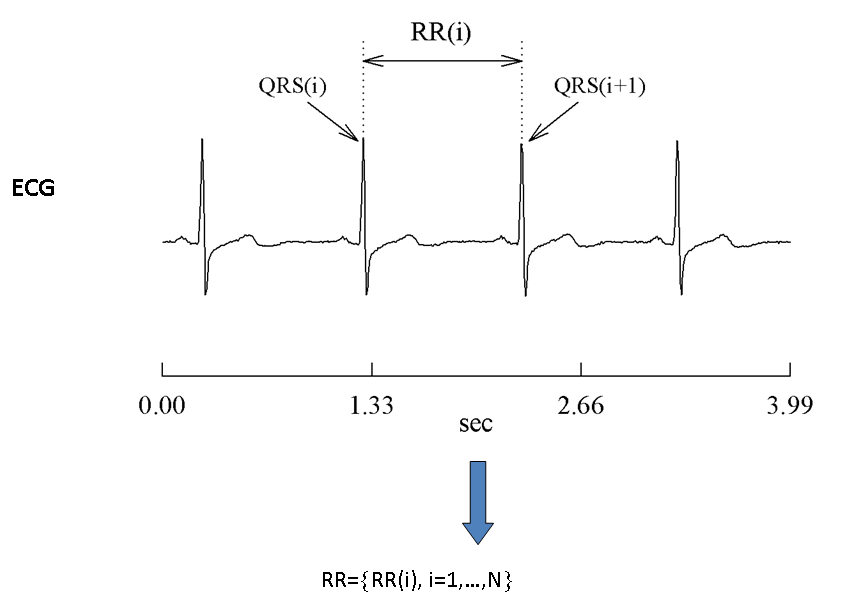
\includegraphics[width=11.97in]{images/RRfig1} 

}

\caption{Definition of Heart Beat Periods.}\label{fig:RRf1}
\end{figure}

\begin{itemize}
\item
  One HBI series is a sample from a male adult, 62 years old (called
  \emph{Jimmy}). Approximately two years before the recording, the
  subject has had a coronary artery bypass, as advised by his physician
  following a diagnosis of congestive heart failure. \emph{Jimmy} used
  antiarrhythmic medicines at the time of measurement.
\item
  Another HBI series is a sample from a healthy male adult, 21 years old
  (called \emph{Tommy}). This subject never reported any cardiac
  complaint. Tommy was playing the piano during the recording.
\item
  A third supposed HBI series is fictitious, and was never recorded from
  a human subject (let's call this counterfeit \emph{Dummy}). Your
  challenge
\end{itemize}

The assignment is to scrutinise the data and find out which time series
belongs to \emph{Jimmy}, \emph{Tommy}, and \emph{Dummy} respectively.
\footnote{The HBI intervals were truncated (not rounded) to a multiple
  of 10 ms (e.g., an interval of 0.457s is represented as 0.450s), and
  to 750 data points each. The means and standard deviations among the
  HBI series are approximately equidistant, which might complicate your
  challenge.}

\subsection{First inspection}\label{first-inspection}

The chances that you are an experienced cardiologist are slim. We
therefore suggest you proceed your detective work as follows:

\begin{itemize}
\tightlist
\item
  Construct a graphical representation of the time series, and inspect
  their dynamics visually (use the code examples provided in the
  \protect\hyperlink{moc1Rsol}{solutions to previous sessions} to plot
  your time series).
\item
  Write down your first guesses about which time series belongs to which
  subject. Take your time for this visual inspection (i.e., which one
  looks more like a line than a plane, which one looks more `smooth'
  than `rough').
\item
  Next, explore some measures of central tendency and dispersion, etc.
\item
  Third, compute the Relative Roughness for each time series, use
  Equation \eqref{eq:RR}
\end{itemize}

\begin{equation}
RR = 2\left[1−\frac{\gamma_1(x_i)}{Var(x_i)}\right]
\label{eq:RR}
\end{equation}

The numerator in the formula stands for the \texttt{lag\ 1}
autocovariance of the HBI time series \(x_i\). The denominator stands
for the (global) variance of \(x_i\). Most statistics packages can
calculate these variances, \texttt{R} and \texttt{Matlab} have built in
functions. Alternatively, you can create the formula yourself.

\begin{itemize}
\tightlist
\item
  Compare your (intuitive) visual inspection with these preliminary
  dynamic quantifications, and find out where each of the HIB series are
  positions on the `colorful spectrum of noises' (i.e., line them up
  with Figure \ref{fig:RRf3}).
\end{itemize}

\begin{figure}

{\centering 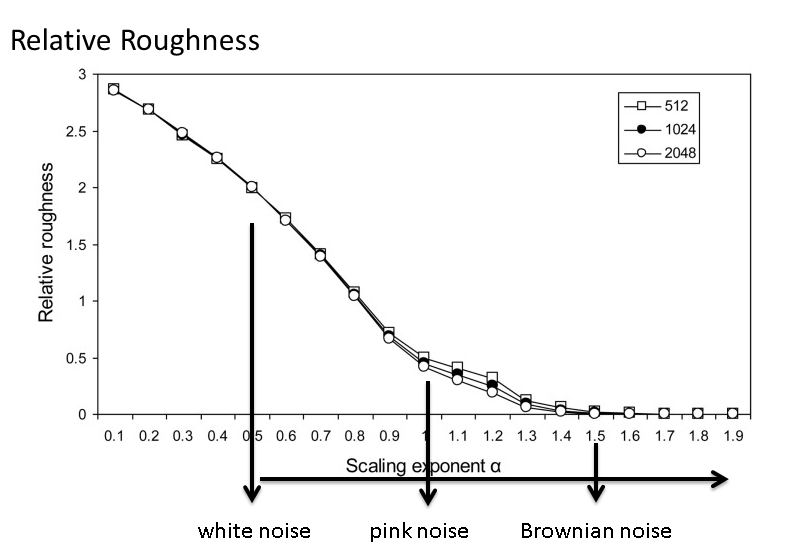
\includegraphics[width=11.01in]{images/RRfig3} 

}

\caption{Coloured Noise versus Relative Roughness}\label{fig:RRf3}
\end{figure}

\subsection{What do we know now, that we didn't knew
before?}\label{what-do-we-know-now-that-we-didnt-knew-before}

Any updates on Jimmy's, Tommy's and Dummy's health? You may start to
wonder about the `meaning' of these dynamics, and not find immediate
answers.

Don't worry; we'll cover the interpretation over the next two weeks in
further depth. Let's focus the dynamics just a little further for now.
It might give you some clues.

\begin{itemize}
\item
  Use the \texttt{randperm} function (in \texttt{Matlab} or in package
  \href{http://www.inside-r.org/packages/cran/pracma}{\texttt{pracma}}
  in \texttt{R}) to randomize the temporal ordering of the HBI series.
\item
  Visualize the resulting time series to check whether they were
  randomized successfully
\item
  Next estimate the Relative Roughness of the randomized series. Did the
  estimates change compared to your previous outcomes (if so, why)?
\item
  Now suppose you would repeat what you did the previous, but instead of
  using shuffle you would integrate the fictitious HBI series (i.e.,
  normalize, then use \texttt{x=cumsum(x))}. You can look up
  \texttt{cumsum} in \texttt{R} or \texttt{Matlab}'s Help
  documentation). Would you get an estimate of Relative Roughness that
  is approximately comparable with what you got in another HBI series?
  If so, why?
\end{itemize}

\protect\hyperlink{hrvsol}{\textbar{} jump to solution \textbar{}}

\section{EXTRA: Creating fractals from random
processes}\label{extra-creating-fractals-from-random-processes}

Below are examples of so-called Iterated Function Systems, copy the code
and run it in \texttt{R} (\texttt{Matlab} scripts are here)

Try to understand what is going on in the two examples below. - How does
the structure come about? We are drawing random numbers! - What's the
difference between the Siepinsky Gasket and the Fern?

\subsection{A Triangle}\label{a-triangle}

\begin{Shaded}
\begin{Highlighting}[]
\CommentTok{# Sierpinski Gasket using Iterated Function Systems}
\CommentTok{#}
\CommentTok{# RM-course Advanced Data Analysis}
\CommentTok{# Module Dynamical and Nonlinear Data analysis and Modeling }
\CommentTok{# }
\CommentTok{# May 2008}
\CommentTok{# Fred Hasselman & Ralf Cox}

\KeywordTok{require}\NormalTok{(dplyr)}

\NormalTok{x =}\StringTok{ }\DecValTok{0}                  \CommentTok{# Starting points}
\NormalTok{y =}\StringTok{ }\DecValTok{0}

\CommentTok{# Emppty plot}
\KeywordTok{plot}\NormalTok{(x,y, }\DataTypeTok{xlim=}\KeywordTok{c}\NormalTok{(}\DecValTok{0}\NormalTok{,}\DecValTok{2}\NormalTok{), }\DataTypeTok{ylim=}\KeywordTok{c}\NormalTok{(}\DecValTok{0}\NormalTok{,}\DecValTok{1}\NormalTok{))}

\NormalTok{for(i in }\DecValTok{1}\NormalTok{:}\DecValTok{20000}\NormalTok{)\{      }\CommentTok{# This takes some time: 20.000 iterations}
  
    \NormalTok{coor=}\KeywordTok{runif}\NormalTok{(}\DecValTok{1}\NormalTok{)       }\CommentTok{# coor becomes a random number between 0 and 1 drawn from the uniform distribution}
    
    \CommentTok{# Equal chances (33%) to perform one of these 3 transformations of x and y}
    \NormalTok{if(coor<=}\FloatTok{0.33}\NormalTok{)\{     }
        \NormalTok{x=}\FloatTok{0.5}\NormalTok{*x}
        \NormalTok{y=}\FloatTok{0.5}\NormalTok{*y}
        \KeywordTok{points}\NormalTok{(x,y,}\DataTypeTok{pch=}\StringTok{"."}\NormalTok{, }\DataTypeTok{col=}\StringTok{"green"}\NormalTok{) }\CommentTok{#plot these points in green}
    \NormalTok{\}}

    \NormalTok{if(}\KeywordTok{between}\NormalTok{(coor,}\FloatTok{0.33}\NormalTok{,}\FloatTok{0.66}\NormalTok{))\{}
        \NormalTok{x=}\FloatTok{0.5}\NormalTok{*x}\FloatTok{+0.5}
        \NormalTok{y=}\FloatTok{0.5}\NormalTok{*y}\FloatTok{+0.5}
        \KeywordTok{points}\NormalTok{(x,y, }\DataTypeTok{pch=}\StringTok{"."}\NormalTok{, }\DataTypeTok{col=}\StringTok{"blue"}\NormalTok{) }\CommentTok{# plot these points in blue}
    \NormalTok{\}}

    \NormalTok{if(coor>}\FloatTok{0.66}\NormalTok{)\{}
        \NormalTok{x=}\FloatTok{0.5}\NormalTok{*x}\DecValTok{+1}
        \NormalTok{y=}\FloatTok{0.5}\NormalTok{*y}
        \KeywordTok{points}\NormalTok{(x,y, }\DataTypeTok{pch=}\StringTok{"."}\NormalTok{, }\DataTypeTok{col=}\StringTok{"red"}\NormalTok{) }\CommentTok{#plot these points in red}
    \NormalTok{\}}
\NormalTok{\} }\CommentTok{# for ...}
\end{Highlighting}
\end{Shaded}

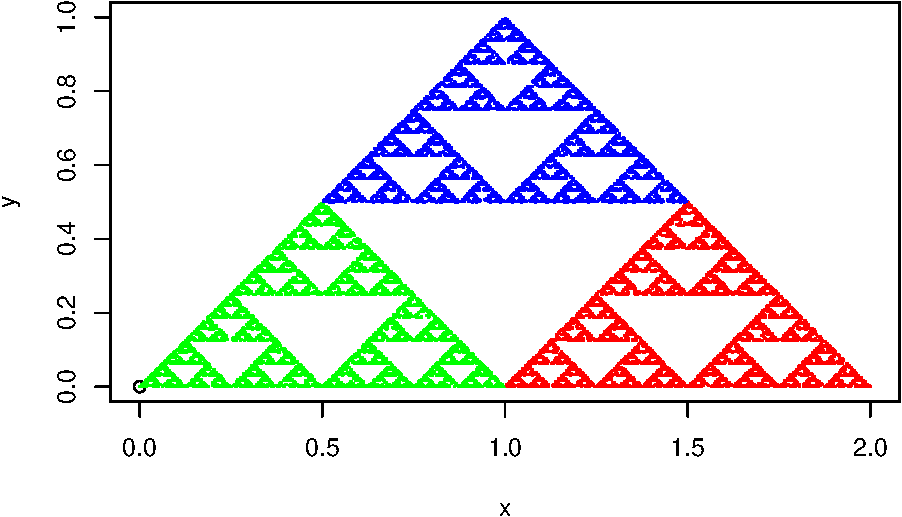
\includegraphics{DCS1617_files/figure-latex/siepinsky-1.pdf}

\subsection{A Fern}\label{a-fern}

\begin{Shaded}
\begin{Highlighting}[]
\CommentTok{# Barnsley's Fern using Iterated Function Systems}
\CommentTok{#}
\CommentTok{# RM-course Advanced Data Analysis}
\CommentTok{# Module Dynamical and Nonlinear Data analysis and Modeling }
\CommentTok{# }
\CommentTok{# May 2008}
\CommentTok{# Fred Hasselman & Ralf Cox}

\KeywordTok{require}\NormalTok{(dplyr)}

\NormalTok{x =}\StringTok{ }\DecValTok{0}                  \CommentTok{# Starting points}
\NormalTok{y =}\StringTok{ }\DecValTok{0}

\CommentTok{# Emppty plot}
\KeywordTok{plot}\NormalTok{(x,y, }\DataTypeTok{pch=}\StringTok{"."}\NormalTok{, }\DataTypeTok{xlim=}\KeywordTok{c}\NormalTok{(-}\DecValTok{3}\NormalTok{,}\DecValTok{3}\NormalTok{), }\DataTypeTok{ylim=}\KeywordTok{c}\NormalTok{(}\DecValTok{0}\NormalTok{,}\DecValTok{12}\NormalTok{))}

\NormalTok{for(i in }\DecValTok{1}\NormalTok{:}\DecValTok{50000}\NormalTok{)\{      }\CommentTok{# This takes some time: 20.000 iterations}
  
    \NormalTok{coor=}\KeywordTok{runif}\NormalTok{(}\DecValTok{1}\NormalTok{)       }\CommentTok{# coor becomes a random number between 0 and 1 drawn from the uniform distribution}
    
    \NormalTok{if(coor<=}\FloatTok{0.01}\NormalTok{)\{                  }\CommentTok{#This transformation 1% of the time}
        \NormalTok{x =}\StringTok{ }\DecValTok{0}
        \NormalTok{y =}\StringTok{ }\FloatTok{0.16} \NormalTok{*}\StringTok{ }\NormalTok{y}
        \KeywordTok{points}\NormalTok{(x,y, }\DataTypeTok{pch=}\StringTok{"."}\NormalTok{, }\DataTypeTok{col=}\StringTok{"green3"}\NormalTok{) }
    \NormalTok{\}}
    
    \NormalTok{if(}\KeywordTok{between}\NormalTok{(coor,}\FloatTok{0.01}\NormalTok{, }\FloatTok{0.08}\NormalTok{))\{   }\CommentTok{#This transformation 7% of the time}
        \NormalTok{x =}\StringTok{ }\FloatTok{0.20} \NormalTok{*}\StringTok{ }\NormalTok{x -}\StringTok{ }\FloatTok{0.26} \NormalTok{*}\StringTok{ }\NormalTok{y}
        \NormalTok{y =}\StringTok{ }\FloatTok{0.23} \NormalTok{*}\StringTok{ }\NormalTok{x +}\StringTok{ }\FloatTok{0.22} \NormalTok{*}\StringTok{ }\NormalTok{y +}\StringTok{ }\FloatTok{1.6}
        \KeywordTok{points}\NormalTok{(x,y, }\DataTypeTok{pch=}\StringTok{"."}\NormalTok{, }\DataTypeTok{col=}\StringTok{"green2"}\NormalTok{) }
    \NormalTok{\}}
    
    \NormalTok{if(}\KeywordTok{between}\NormalTok{(coor,}\FloatTok{0.08}\NormalTok{,}\FloatTok{0.15}\NormalTok{))\{   }\CommentTok{#This transformation 7% of the time}
        \NormalTok{x =}\StringTok{ }\NormalTok{-}\FloatTok{0.15} \NormalTok{*}\StringTok{ }\NormalTok{x +}\StringTok{ }\FloatTok{0.28} \NormalTok{*}\StringTok{ }\NormalTok{y}
        \NormalTok{y =}\StringTok{  }\FloatTok{0.26} \NormalTok{*}\StringTok{ }\NormalTok{x +}\StringTok{ }\FloatTok{0.24} \NormalTok{*}\StringTok{ }\NormalTok{y +}\StringTok{ }\FloatTok{0.44}
       \KeywordTok{points}\NormalTok{(x,y, }\DataTypeTok{pch=}\StringTok{"."}\NormalTok{, }\DataTypeTok{col=}\StringTok{"springgreen3"}\NormalTok{)}
    \NormalTok{\}}
    
    \NormalTok{if(coor>}\FloatTok{0.15}\NormalTok{)\{      }\CommentTok{#This transformation 85% of the time}
        \NormalTok{x =}\StringTok{  }\FloatTok{0.85} \NormalTok{*}\StringTok{ }\NormalTok{x +}\StringTok{ }\FloatTok{0.04} \NormalTok{*}\StringTok{ }\NormalTok{y}
        \NormalTok{y=}\StringTok{  }\NormalTok{-}\FloatTok{0.04} \NormalTok{*}\StringTok{ }\NormalTok{x +}\StringTok{ }\FloatTok{0.85} \NormalTok{*}\StringTok{ }\NormalTok{y +}\StringTok{ }\FloatTok{1.6} 
        \KeywordTok{points}\NormalTok{(x,y, }\DataTypeTok{pch=}\StringTok{"."}\NormalTok{, }\DataTypeTok{col=}\StringTok{"springgreen2"}\NormalTok{)}
    \NormalTok{\}}
    
\NormalTok{\} }\CommentTok{# for ...}
\end{Highlighting}
\end{Shaded}

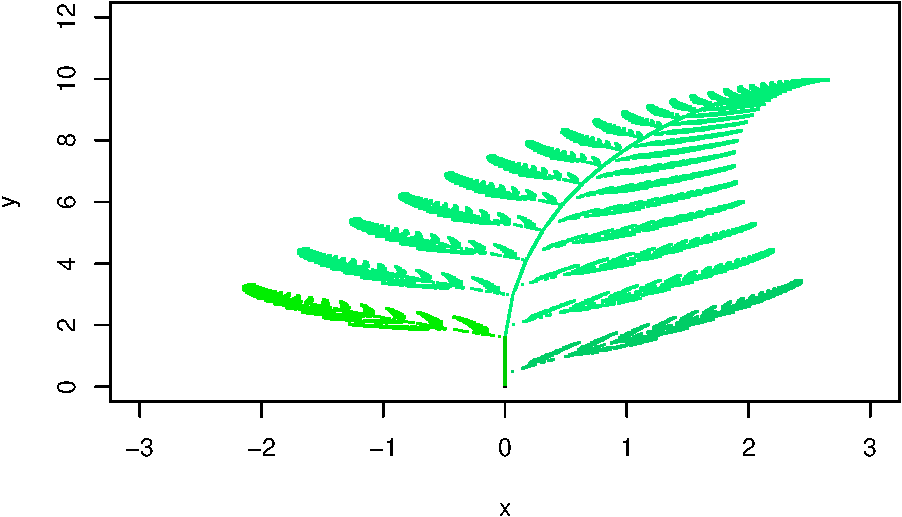
\includegraphics{DCS1617_files/figure-latex/fern-1.pdf}

\subsection{The fractal / chaos game}\label{the-fractal-chaos-game}

These
\href{https://en.wikipedia.org/wiki/Iterated_function_system}{Iterated
Function Systems} also go by the name of `the fractal game' and are used
in computer science, the gaming industry, graphic design, etc.

EXTRA-EXTRA: This Wikipedia page on
\href{https://en.wikipedia.org/wiki/Barnsley_fern}{Barnsley's fern} has
some good info on the topic. At the end they display \emph{Mutant
varieties}. Try to implement them!

You can by now probably guess that the these simple rules can be
described as constraints on the degrees of freedom of the system. Like
with the models of growth we simulated, the rules of the fractal game
can be made dependent on other processes or events. A great example are
the so-called \href{https://en.wikipedia.org/wiki/Fractal_flame}{fractal
flames} implemented in a screen-saver called
\href{http://www.electricsheep.org}{\emph{electric sheep}}, which
combines genetic algorithms, distributed computind and user input
(``likes'') to create intruiging visual patterns on your computer
screen.\footnote{Use at your own risk! You will find yourself silently
  staring at the screen for longer periods of time.}

\chapter{\texorpdfstring{\textbf{Fluctuation and Disperion analyses
I}}{Fluctuation and Disperion analyses I}}\label{fda1}

\BeginKnitrBlock{rmdimportant}
Before you begin, look at the notes for
\protect\hyperlink{lecture-4}{Lecture 4}.
\EndKnitrBlock{rmdimportant}

\hypertarget{psd}{\section{Assignment: The Spectral Slope}\label{psd}}

We can use the power spectrum to estimate a \textbf{self-affinity
parameter}, or scaling exponent.

\begin{itemize}
\tightlist
\item
  Download \texttt{ts1.txt}, \texttt{ts2.txt}, \texttt{ts3.txt}
  \href{https://github.com/FredHasselman/DCS/tree/master/assignmentData/Fluctuation_PSDslope}{here}.
  If you use \texttt{R} and have package \texttt{rio} installed you can
  run this code. It loads the data into a \texttt{data.frame} object
  directly from \texttt{Github}.
\end{itemize}

\begin{Shaded}
\begin{Highlighting}[]
\KeywordTok{library}\NormalTok{(rio)}
\NormalTok{TS1 <-}\StringTok{ }\NormalTok{rio::}\KeywordTok{import}\NormalTok{(}\StringTok{"https://raw.githubusercontent.com/FredHasselman/DCS/master/assignmentData/Fluctuation_PSDslope/ts1.txt"}\NormalTok{)}
\NormalTok{TS2 <-}\StringTok{ }\NormalTok{rio::}\KeywordTok{import}\NormalTok{(}\StringTok{"https://raw.githubusercontent.com/FredHasselman/DCS/master/assignmentData/Fluctuation_PSDslope/ts2.txt"}\NormalTok{)}
\NormalTok{TS3 <-}\StringTok{ }\NormalTok{rio::}\KeywordTok{import}\NormalTok{(}\StringTok{"https://raw.githubusercontent.com/FredHasselman/DCS/master/assignmentData/Fluctuation_PSDslope/ts3.txt"}\NormalTok{)}

\CommentTok{# These objects are now data.frames with one column named V1. }
\CommentTok{# If you want to change the column names}
\KeywordTok{colnames}\NormalTok{(TS1) <-}\StringTok{ "TS1"}
\KeywordTok{colnames}\NormalTok{(TS2) <-}\StringTok{ "TS2"}
\KeywordTok{colnames}\NormalTok{(TS3) <-}\StringTok{ "TS3"}
\end{Highlighting}
\end{Shaded}

\begin{itemize}
\tightlist
\item
  Plot the three `raw' time series.
\end{itemize}

\subsection{Basic data checks and
preparations}\label{basic-data-checks-and-preparations}

For spectral analysis we need to check some data assumptions (see
\protect\hyperlink{data-considerations}{notes on data preparation,
Lecture 4}).

\subsubsection*{Normalize}\label{normalize}
\addcontentsline{toc}{subsubsection}{Normalize}

\begin{enumerate}
\def\labelenumi{\arabic{enumi}.}
\tightlist
\item
  Are the lengths of the time series a power of 2? (Use
  \texttt{log2(length\ of\ var)} )
\end{enumerate}

\begin{itemize}
\tightlist
\item
  Computation of the frequency domain is greatly enhanced if data length
  is a power (of 2).
\end{itemize}

\begin{enumerate}
\def\labelenumi{\arabic{enumi}.}
\setcounter{enumi}{1}
\tightlist
\item
  Are the data normalized? (we will \emph{not} remove datapoints outside
  3SD)

  \begin{itemize}
  \tightlist
  \item
    To normalize we have to subtract the mean from each value in the
    time series and divide it by the standard deviation, the function
    \texttt{scale()} can do this for you, but you could also use
    \texttt{mean()} and \texttt{sd()} to construct your own function.
  \end{itemize}
\item
  Plot the normalized time series.
\end{enumerate}

\subsubsection*{Detrend}\label{detrend}
\addcontentsline{toc}{subsubsection}{Detrend}

Before a spectral analysis you should remove any linear trends (it
cannot deal with nonstationary signals!)

\begin{enumerate}
\def\labelenumi{\arabic{enumi}.}
\tightlist
\item
  Detrend the normalized data (just the linear trend).

  \begin{itemize}
  \tightlist
  \item
    This can be done using the function \texttt{pracma::detrend()}.
  \item
    Extra: Try to figure out how to detrend the data using
    \texttt{stats::lm()} or \texttt{stats::poly()}
  \end{itemize}
\item
  Plot the detrended data.
\end{enumerate}

\subsubsection*{Get the log-log slope in Power Spectral
Density}\label{get-the-log-log-slope-in-power-spectral-density}
\addcontentsline{toc}{subsubsection}{Get the log-log slope in Power
Spectral Density}

The function \texttt{fd.psd()} will perform the spectral slope fitting
procedure.

\begin{enumerate}
\def\labelenumi{\arabic{enumi}.}
\tightlist
\item
  Look at the manual pages to figure out how to call the function. The
  manual is on blackboard and
  \href{https://github.com/FredHasselman/DCS/blob/master/functionLib/}{Github}

  \begin{itemize}
  \tightlist
  \item
    Remember, we have already normalized and detrended the data.
  \item
    You can also look at the code itself by selecting the function name
    in\texttt{R} and pressing \texttt{F2}
  \end{itemize}
\item
  Calculate the spectral slopes for the three normalized and detrended
  time series.

  \begin{itemize}
  \tightlist
  \item
    Call with \texttt{plot\ =\ TRUE}
  \item
    Compare the results\ldots{} What is your conclusion?
  \end{itemize}
\end{enumerate}

\protect\hyperlink{psdsol}{\textbar{} jump to solution \textbar{}}

\section{DFA and SDA}\label{dfa}

\begin{itemize}
\tightlist
\item
  Use the functions \texttt{fd.dfa()} and \texttt{fd.sda()} to estimate
  the self-affinity parameter and Dimension of the series.

  \begin{itemize}
  \tightlist
  \item
    Check what kind of data preparation is required for SDA and DFA in
    \protect\hyperlink{data-considerations}{notes on data preparation,
    Lecture 4}.
  \item
    Compare the results between the three different methods.
  \end{itemize}
\end{itemize}

\protect\hyperlink{dfasol}{\textbar{} jump to solution \textbar{}}

\section{ACF/PACF, Relative Roughness}\label{pacfrel}

\begin{itemize}
\tightlist
\item
  Also calculate the ACF, PACF (\protect\hyperlink{pacf}{see
  assignment}) and \protect\hyperlink{relR}{Relative Roughness}

  \begin{itemize}
  \tightlist
  \item
    Compare the results.
  \end{itemize}
\end{itemize}

\protect\hyperlink{pacfrelrsol}{\textbar{} jump to solution \textbar{}}

\section{Heartbeat dynamics II}\label{hrv2}

In the \protect\hyperlink{relR}{previous assignment}, you were presented
with three different time series of heartbeat intervals (HBI), and you
analyzed them using a measure of Relative Roughness (RR; cf.~Marmelat \&
Delignières, 2012).

A logical step is to unleash the full force of your new analytic toolbox
onto the HBI series.

\begin{itemize}
\tightlist
\item
  Keep track of the outcomes of each time series for 4 different
  analyses (RR, PSD, SDA, DFA).

  \begin{itemize}
  \tightlist
  \item
    Do the outcomes of the different methods converge on the continuum
    of blue, white and pink, to Brownian and black noise? That is, do
    they indicate the same type of temporal structure?
  \end{itemize}
\item
  As a final step, construct return plots for each time series and try
  to interpret what you observe, given the outcomes of the scaling
  parameter estimates.
\end{itemize}

\protect\hyperlink{hrv2sol}{\textbar{} jump to solution \textbar{}}

\section{Analysis of Deterministic Chaos}\label{chaos}

\begin{itemize}
\tightlist
\item
  Generate a chaotic timeseries (e.g. \(r = 4\) ) of equal length as the
  time series used above (use the function
  \texttt{growth.ac(\ ...,\ type\ =\ "logistic")} in
  \texttt{nlRtsa\_SOURCE}, see the
  \protect\hyperlink{linear-and-logistic-growth}{solutions of Lecture 1
  and 2})

  \begin{itemize}
  \tightlist
  \item
    This is in fact one of the series you analysed in a
    \protect\hyperlink{pacf}{previous assignment}. If you still have the
    results use them for the next part.
  \end{itemize}
\item
  Get all the scaling quantities for this series as well as the ACF and
  PACF and \protect\hyperlink{the-return-plot}{some return plots} just
  like in the previous assignments.

  \begin{itemize}
  \tightlist
  \item
    Compare the results to e.g.~the heartbeat series.
  \end{itemize}
\end{itemize}

\protect\hyperlink{chaossol}{\textbar{} jump to solution \textbar{}}

\chapter{Fluctuation and Disperion analyses II}\label{fda2}

There were no assignments for this Lecture.

\chapter{\texorpdfstring{\textbf{Phase Space Reconstruction and
RQA}}{Phase Space Reconstruction and RQA}}\label{RQA}

You can use \texttt{R} or \texttt{Matlab} to run \texttt{RQA} analyses.
This document is based on \texttt{R}. You can find the assignments for
\texttt{Matlab} on Blackboard.

\textbf{Packages for Phase Space Reconstruction}

We'll use package \texttt{fractal} and \texttt{rgl} to reconstruct some
phase spaces.

\begin{itemize}
\tightlist
\item
  If you have sourced the functions in \texttt{nlRtsa\_SOURCE.R} you can
  install and load these packages by running:
  \texttt{in.IT(c("fractal","rgl"))}. The function \texttt{in.IT()} will
  first check if the requested packages are installed on the machine and
  only install them if they are not present.
\end{itemize}

\section{Reconstruct the Lorenz
attractor}\label{reconstruct-the-lorenz-attractor}

\begin{itemize}
\tightlist
\item
  Package fractal includes the 3 dimensions of the Lorenz system in the
  chaotic regime.

  \begin{itemize}
  \tightlist
  \item
    Run this code \texttt{plot3d(lorenz)} to get an interactive 3D plot
    \footnote{You'll need the \href{http://www.x.org/wiki/}{X Window
      System} for interactive 3D plotting. This Linux desktop system
      comes installed in some way or form on most Mac and Windows
      systems.} of this strange attractor.
  \end{itemize}
\end{itemize}

\begin{quote}
NOTE: Package \texttt{fractal} and package \texttt{nonlinearTseries} use
functions with similar names, do not load them together.
\end{quote}

We'll reconstruct the attractor based on just dimension \texttt{X} of
the system.

\begin{itemize}
\tightlist
\item
  Use \texttt{lx\ \textless{}-\ lorenz{[}1:2048,1{]}} to reconstruct the
  phase space.

  \begin{itemize}
  \tightlist
  \item
    Find an optimal embedding lag using \texttt{timeLag()}, use
    \texttt{method\ =\ "mutual"}.
  \item
    Find the embedding dimension, using \texttt{FNN()}
  \item
    Embed the timeseries using \texttt{embedSeries()}.
  \item
    Plot the reconstructed phase space. (You'll need to use
    \texttt{as.matrix()} on the object created by
    \texttt{embedSeries()})

    \begin{itemize}
    \tightlist
    \item
      Use \texttt{rgl::open3d()} to open an interactive plotting device
      if you like.
    \end{itemize}
  \end{itemize}
\end{itemize}

\section{Reconstruct the Predator-Prey
model}\label{reconstruct-the-predator-prey-model}

Use the same procedure as above to reconstruct the state space of the
predator-prey system. (Look \protect\hyperlink{ppdsol}{at the solutions}
to get a \texttt{Foxes} or \texttt{Rabbit} series).

\begin{itemize}
\tightlist
\item
  You should get a 2D state space, so 3D plotting might be a bit too
  much for this system.
\end{itemize}

\section{Assignment: (auto-) Recurrence Quantification
Analysis}\label{assignment-auto--recurrence-quantification-analysis}

There are several packages which can perform (C)RQA analysis, we'll use
\href{https://cran.r-project.org/web/packages/crqa/index.html}{\texttt{crqa}}
because it can perform both continuous and categorical analyses. If you
only have continuous data, you migh be better off using package
\href{https://cran.r-project.org/web/packages/nonlinearTseries/index.html}{\texttt{nonlinearTseries}},
in this course we will only use package \texttt{crqa}.

\begin{quote}
NOTE: Package \texttt{crqa()} was designed to run categorical
Cross-Recurrence Quantification Analysis (see
\href{http://journal.frontiersin.org/Journal/10.3389/fpsyg.2014.00510/abstract}{Coco
\& Dale (2014)} and for R code see appendices in
\href{http://arxiv.org/abs/1310.0201}{Coco \& Dale (2013)}). We can
trick it to run auto-RQA by providing the same timeseries for
\texttt{ts1} and \texttt{ts2} and setting the parameter \texttt{side} to
either \texttt{"upper"} or \texttt{"lower"}
\end{quote}

\begin{itemize}
\tightlist
\item
  Perform an RQA on the reconstructed state space of the Lorenz system.

  \begin{itemize}
  \tightlist
  \item
    You'll need a radius (also called: threshold) in order to decide
    which points are close together (recurrent).

    \begin{itemize}
    \tightlist
    \item
      \texttt{crqa} provides a function which will automatically select
      the best parameter settings: \texttt{optimizeParam()}
    \item
      Best way to ensure you are using the same parameters in each
      function is to create some lists with parameter settings (check
      the \texttt{crqa} manual to figure out what these parameters
      mean):
    \end{itemize}
  \end{itemize}
\end{itemize}

\begin{Shaded}
\begin{Highlighting}[]
\CommentTok{# General settings for `crqa()`}
\NormalTok{par0 <-}\StringTok{ }\KeywordTok{list}\NormalTok{(}\DataTypeTok{rescale =} \DecValTok{1}\NormalTok{,}
             \DataTypeTok{normalize =} \DecValTok{0}\NormalTok{,}
             \DataTypeTok{mindiagline =} \DecValTok{2}\NormalTok{,}
             \DataTypeTok{minvertline =} \DecValTok{2}\NormalTok{,}
             \DataTypeTok{tw =} \DecValTok{0}\NormalTok{,}
             \DataTypeTok{whiteline =} \OtherTok{FALSE}\NormalTok{,}
             \DataTypeTok{recpt =} \OtherTok{FALSE}\NormalTok{,}
             \DataTypeTok{side =} \StringTok{"lower"}\NormalTok{,}
             \DataTypeTok{checkl =} \KeywordTok{list}\NormalTok{(}\DataTypeTok{do =} \OtherTok{FALSE}\NormalTok{, }\DataTypeTok{thrshd =} \DecValTok{3}\NormalTok{, }\DataTypeTok{datatype =} \StringTok{"categorical"}\NormalTok{,}\DataTypeTok{pad =} \OtherTok{TRUE}\NormalTok{)}
             \NormalTok{)}

\CommentTok{# Settings for `optimizeParam()`}
\NormalTok{par <-}\StringTok{ }\KeywordTok{list}\NormalTok{(}\DataTypeTok{lgM =}  \DecValTok{20}\NormalTok{, }\DataTypeTok{steps =} \KeywordTok{seq}\NormalTok{(}\DecValTok{1}\NormalTok{, }\DecValTok{6}\NormalTok{, }\DecValTok{1}\NormalTok{),}
           \DataTypeTok{radiusspan =} \DecValTok{100}\NormalTok{, }\DataTypeTok{radiussample =} \DecValTok{40}\NormalTok{,}
           \DataTypeTok{normalize =} \NormalTok{par0$normalize, }
           \DataTypeTok{rescale =} \NormalTok{par0$rescale, }
           \DataTypeTok{mindiagline =} \NormalTok{par0$mindiagline, }\DataTypeTok{minvertline =} \NormalTok{par0$minvertline,}
           \DataTypeTok{tw =} \NormalTok{par0$tw, }
           \DataTypeTok{whiteline =} \NormalTok{par0$whiteline, }
           \DataTypeTok{recpt =} \NormalTok{par0$recpt, }
           \DataTypeTok{fnnpercent =} \DecValTok{10}\NormalTok{, }\DataTypeTok{typeami =} \StringTok{"mindip"}\NormalTok{)}
\end{Highlighting}
\end{Shaded}

\begin{itemize}
\tightlist
\item
  Get the optimal parameters using a radius which will give us 2\%-5\%
  recurrent points.
\end{itemize}

\begin{Shaded}
\begin{Highlighting}[]
\NormalTok{ans <-}\StringTok{ }\KeywordTok{optimizeParam}\NormalTok{(}\DataTypeTok{ts1 =} \NormalTok{lx, }\DataTypeTok{ts2 =} \NormalTok{lx, }\DataTypeTok{par =} \NormalTok{par, }\DataTypeTok{min.rec =} \DecValTok{2}\NormalTok{, }\DataTypeTok{max.rec =} \DecValTok{5}\NormalTok{)}
\end{Highlighting}
\end{Shaded}

\begin{itemize}
\tightlist
\item
  Run the RQA analysis using the same settings with which the parameters
  were found.
\end{itemize}

\begin{Shaded}
\begin{Highlighting}[]
\NormalTok{crqaOutput <-}\StringTok{ }\KeywordTok{crqa}\NormalTok{(}\DataTypeTok{ts1 =} \NormalTok{lx, }\DataTypeTok{ts2 =} \NormalTok{lx, }
                  \DataTypeTok{delay =} \NormalTok{ans$delay, }
                  \DataTypeTok{embed =} \NormalTok{ans$emddim, }
                  \DataTypeTok{radius =} \NormalTok{ans$radius, }
                  \DataTypeTok{normalize =} \NormalTok{par0$normalize,}
                  \DataTypeTok{rescale =} \NormalTok{par0$rescale, }
                  \DataTypeTok{mindiagline =} \NormalTok{par0$mindiagline, }\DataTypeTok{minvertline =} \NormalTok{par0$minvertline,}
                  \DataTypeTok{tw =} \NormalTok{par0$tw, }
                  \DataTypeTok{whiteline =} \NormalTok{par0$whiteline, }
                  \DataTypeTok{recpt =} \NormalTok{par0$recpt, }
                  \DataTypeTok{side =} \NormalTok{par0$side, }\DataTypeTok{checkl =} \NormalTok{par0$checkl}
                  \NormalTok{)}
\end{Highlighting}
\end{Shaded}

\begin{itemize}
\tightlist
\item
  The output of \texttt{crqa} is a list with recurrence measures, the
  last entry is the recurrence plot. It is represented as a so-called
  \texttt{sparse-matrix}.

  \begin{itemize}
  \tightlist
  \item
    This representation severely decreases the amount of memory occupied
    by the recurrence matrix. It is basically a list of indices of cells
    that contain a \(1\). The \(0\) do not need to be stored.
  \item
    In order to plot this matrix you could use \texttt{image()}, but
    this does not produce the recurrence plot as they are usually
    displayed, the y-axis needs to be flipped.
  \item
    We created a function which will take as input the list output of
    \texttt{crqa}, which wil be used to plot the recurrence matrix. If
    you have sourced the \texttt{nlRtsa} functions you can call
    \texttt{plotRP.crqa(crqaOutput)}.
  \end{itemize}
\end{itemize}

\section{Assignment: RQA of circle-tracing
data}\label{assignment-rqa-of-circle-tracing-data}

\chapter{\texorpdfstring{\textbf{Categorical and Cross-RQA
(CRQA)}}{Categorical and Cross-RQA (CRQA)}}\label{CRQA}

\chapter{Potential and Catasrophe Models}\label{cusp}

\chapter{Complex Networks}\label{nets}

\part{Lecture Notes}\label{part-lecture-notes}

\chapter*{Lecture 1}\label{lecture-1}
\addcontentsline{toc}{chapter}{Lecture 1}

\section*{Modeling change processes in
1D}\label{modeling-change-processes-in-1d}
\addcontentsline{toc}{section}{Modeling change processes in 1D}

The simplest non-trivial \emph{iterative change process} can be
described by the following \emph{difference equation}:

\begin{equation}
Y_{t+1} = Y_{t=0} + a*Y_t
\label{eq:lin}
\end{equation}

Equation \eqref{eq:lin} describes the way in which the value of \(Y\)
changes
\href{https://en.wikipedia.org/wiki/Discrete_time_and_continuous_time}{between
two adjacent, discrete moments in time} (hence the term
\href{https://en.wikipedia.org/wiki/Recurrence_relation}{difference
equation, or recurrence relation}). There are two parameters resembling
an intercept and a slope:

\begin{enumerate}
\def\labelenumi{\arabic{enumi}.}
\tightlist
\item
  The starting value \(Y_0\) at \(t=0\), also called the \emph{starting
  value}, or the \emph{initial conditions}.
\item
  A rule for incrementing time, here the change in \(Y\) takes place
  over a discrete time step of 1: \(t+1\).
\end{enumerate}

The values taken on by variable \(Y\) are considered to represent the
states quantifiable observable leAlternative ways to describe the change
of states :

\begin{itemize}
\tightlist
\item
  A dynamical rule describing the propagation of the states of a system
  observable measured by the values of variable \texttt{Y} through
  discrete time.
\item
  A dynamic law describing the time-evolution of the states of a system
  observable measured by the variable \texttt{Y}.
\end{itemize}

These descriptions all refer to the change processes that govern system
observables (properties of dynamical systems that can be observed
through measurement).

\subsection*{\texorpdfstring{\textbf{It's a line! It's a
plane!}}{It's a line! It's a plane!}}\label{its-a-line-its-a-plane}
\addcontentsline{toc}{subsection}{\textbf{It's a line! It's a plane!}}

The formula resembles the equation of a line. There is a constant value
\(Y_{0}\) which is added to a proportion of the value of \(Y\) at time
\(t\), given by parameter \(a\). This is equivalent to the slope of a
line. However, in a \((X,Y)\) plane there are two `spatial' (metric)
dimensions representing the values two variables \(X\) and \(Y\) can
take on (see figure).

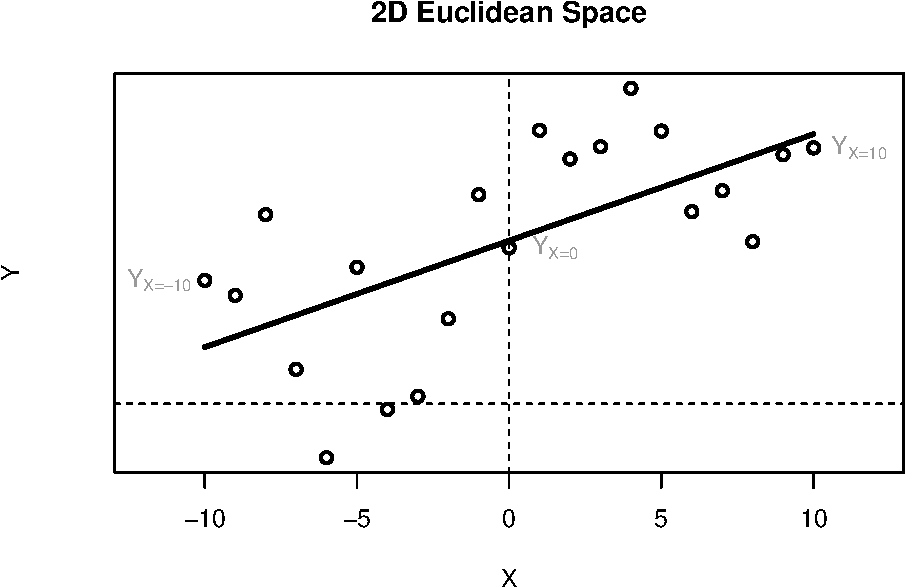
\includegraphics{DCS1617_files/figure-latex/unnamed-chunk-13-1.pdf}

The best fitting straight line would be called a statistical model of
the linear relationship between the observed values of \(X\) and \(Y\).
It can be obtained by fitting a General Linear Model (GLM) to the data.
If \(X\) were to represent repeated measurements the multivariate GLM
for repeated measures would have to be fitted to the data. This can be
very problematic, because statistical models rely on
\href{https://en.wikipedia.org/wiki/Ergodic_theory}{Ergodic theory}:

\begin{quote}
``\ldots{} it is the study of the long term average behavior of systems
evolving in time.'' \footnote{See Dajani \& Dirksin (2008, p.~5,
  \href{http://www.staff.science.uu.nl/~kraai101/lecturenotes2009.pdf}{``A
  simple introduction to Ergodic Theory''})}
\end{quote}

need to assume independence of measurements within and between subjects.
These assumptions can be translated to certain conditions that must hold
for the model to be valid, known as \emph{Compound Symmetry} and
\emph{Sphericity}:

\begin{quote}
The compound symmetry assumption requires that the variances (pooled
within-group) and covariances (across subjects) of the different
repeated measures are homogeneous (identical). This is a sufficient
condition for the univariate F test for repeated measures to be valid
(i.e., for the reported F values to actually follow the F distribution).
However, it is not a necessary condition. The sphericity assumption is a
necessary and sufficient condition for the F test to be valid; it states
that the within-subject ``model'' consists of independent (orthogonal)
components. The nature of these assumptions, and the effects of
violations are usually not well-described in ANOVA textbooks; \footnote{\href{https://www.statsoft.com/Textbook/ANOVA-MANOVA\#sphericity}{Retreived
  from www.statsoft.com}}
\end{quote}

As you can read in the quoted text above, these conditions must hold in
order to be able to identify unique independent components as the
sources of variation of \(Y\) over time within a subject. This is the a
clear example of:

\begin{quote}
It is the theory that decides what we may observe \footnote{Einstein as
  quoted by Heisenberg.}
\end{quote}

If you choose to use GLM repeated measures to model change over time,
you will only be able to infer independent components that are
responsible for the time-evolution of \(Y\). As is hinted in the last
sentence of the quote, the validity of such inferences is not a common
topic of discussion statistics textbooks.

\subsection*{\texorpdfstring{\textbf{No! \ldots{} It's a time
series!}}{No! \ldots{} It's a time series!}}\label{no-its-a-time-series}
\addcontentsline{toc}{subsection}{\textbf{No! \ldots{} It's a time
series!}}

The important difference between a regular 2-dimensional Euclidean plane
and the space in which we model change processes is that the \(X\)-axis
represents the physical dimension \textbf{time}. In the case of the
Linear Map we have a 1D space with one `spatial' dimension \(Y\) and a
time dimension \(t\). This is called
\href{https://en.wikipedia.org/wiki/Time_series}{time series} if \(Y\)
is sampled as a continuous process, or a trial series if the time
between subsequent observations is not relevant, just the fact that
there was a temporal order (for example, a series of response latencies
to trials in a psychological experiment in the order in which they were
presented to the subject).

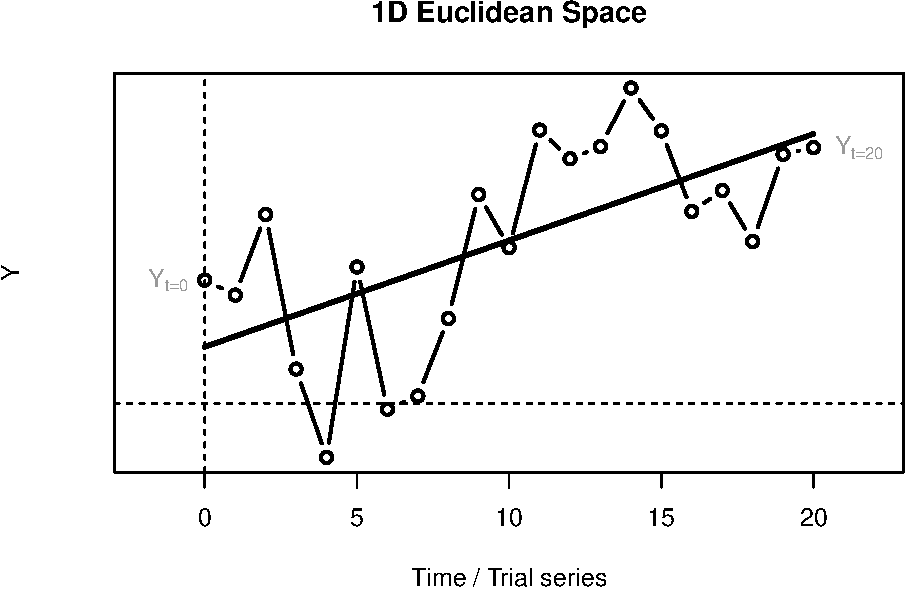
\includegraphics{DCS1617_files/figure-latex/unnamed-chunk-14-1.pdf}

Time behaves different from a spatial dimension in that it is
directional (time cannot be reversed), it cannot take on negative
values, and, unless one is dealing with a truly random process, there
will be a temporal correlation across one or more values of \(Y\)
seperated by an amount of time. In the linear difference equation this
occurs because each value one step in the future is calculated based on
the current value. If the values of \(Y\) represent an observable of a
dynamical system, the system can be said to have a history, or a memory.
Ergodic systems do not have a history or a memory that extends across
more than one time step. This is very convenient, because one can
calculate the expected value of a system observable given infinite time,
by making use of of the laws of probabilities of random events (or
random fields). This means: The average of an observable of an Ergodic
system measured across infinite time (its entire history, the
\textbf{time-average}), will be the be the same value as the average of
this observable measured at one instance in time, but in an infinite
amount of systems of the same kind (the population, the \textbf{spatial
average}) \footnote{In other words: If you throw 1 die 100 times in a
  row, the average of the 100 numbers is the \textbf{time-average} of
  one of the observables of die-throwing systems. If this system is
  ergodic, then its \textbf{time-average} is expected to be similar to
  the average of the numbers that turn up if you throw 100 dice all at
  the same instance of time. The dice layed out on the table represent a
  spatial sample, a snapshot frozen in time, of the possible states the
  system can be in. Taking the average would be the \textbf{spatial
  average} this observable of die-throwing systems. This ergodic
  condiciotn is often implicitly assumed in Behavioural Science when
  studies claim to study change by taking different samples of
  individuals (snapshots of system states) and comparing if they are the
  same.}.

The simple linear difference equation will have a form of *perfect
memory' across the smallest time scale (i.e., the increment of 1,
\(t+1\)). This `memory' concerns a correlation of 1 between values at
adjacent time points (a short range temporal correlation, SRC), because
the change from \(Y_t\) to \(Y_{t+1}\) is exactly equal to \(a * Y_t\)
at each iteration step. This is the meaning of deterministic, not that
each value of \(Y\) is the same, but that the value of \(Y\) now can be
perfectly explained form the value of \(Y\) one moment in the past.

Summarising, the most profound difference is not the fact that the
equation of linear change is a deterministic model and the GLM is a
probabilistic model with parameters fitted from data, this is something
we can (and will) do for \(a\) as well. The profound difference between
the models is the role given to the passage of time:

\begin{itemize}
\tightlist
\item
  The linear difference equation represents changes in \(Y\) as a
  function of the physical dimension \emph{time} and \(Y\) itself.
\item
  The GLM represents changes in \(Y\) as a function of a
  \href{https://en.wikipedia.org/wiki/Linear_predictor_function}{linear
  predictor} composed of additive components that can be regarded as
  independent sources of variation that sum up to the observed values of
  \(Y\).
\end{itemize}

\chapter*{Lecture 2}\label{lecture-2}
\addcontentsline{toc}{chapter}{Lecture 2}

\section*{Numerical integration}\label{numerical-integration}
\addcontentsline{toc}{section}{Numerical integration}

In order to `solve' a differential equation for continuous time using a
method of numerical integration, one could code it like in the
spreadsheet assignment below. For \texttt{R} and \texttt{Matlab} there
are so-called \emph{solvers} available, functions that will do the
integration for you. For \texttt{R} look at the
\href{http://desolve.r-forge.r-project.org}{Examples in package
\texttt{deSolve}}.

\subsection*{Euler's method and
more\ldots{}}\label{eulers-method-and-more}
\addcontentsline{toc}{subsection}{Euler's method and more\ldots{}}

The result of applying a method of numerical integration is called a
\textbf{numerical solution} of the differential equation. The
\textbf{analytical solution} is the equation which will give you a value
of \(Y\) for any point in time, given an initial value \(Y_0\). Systems
which have an analytical solution can be used to test the accuracy of
\textbf{numerical solutions}.

\subsubsection*{Analytical solution}\label{analytical-solution}
\addcontentsline{toc}{subsubsection}{Analytical solution}

Remember that the analytical solution for the logistic equation is:

\[
Y(t)  =  \frac{K}{1 + \left(\frac{K}{Y_{0} - 1}\right) * e^{-r*t} }
\]

If we want to know the growth level \(Y_t\) at \(t=10\), with
\(Y_0=.0001\), \(r=1.1\) and \(K=4\), we can just \texttt{fill\ it\ in}:

\begin{Shaded}
\begin{Highlighting}[]
\CommentTok{# Define a function for the solution}
\NormalTok{logSol <-}\StringTok{ }\NormalTok{function(Y0, r, K, t)\{K/(}\DecValTok{1}\NormalTok{+(K/Y0}\DecValTok{-1}\NormalTok{)*}\KeywordTok{exp}\NormalTok{(-r*t))\}}

\CommentTok{# Call the function}
\KeywordTok{logSol}\NormalTok{(}\DataTypeTok{Y0=}\NormalTok{.}\DecValTok{0001}\NormalTok{, }\DataTypeTok{r=}\FloatTok{1.1}\NormalTok{, }\DataTypeTok{K=}\DecValTok{4}\NormalTok{, }\DataTypeTok{t=}\DecValTok{10}\NormalTok{)}
\end{Highlighting}
\end{Shaded}

\begin{verbatim}
## [1] 2.398008
\end{verbatim}

We can pas a vector of timepoints to create the exact solution, the same
we would get if we were to iterate the differential/difference equation.

\begin{Shaded}
\begin{Highlighting}[]
\CommentTok{# Plot from t=1 to t=100}
\KeywordTok{plot}\NormalTok{(}\KeywordTok{logSol}\NormalTok{(}\DataTypeTok{Y0=}\NormalTok{.}\DecValTok{0001}\NormalTok{, }\DataTypeTok{r=}\FloatTok{1.1}\NormalTok{, }\DataTypeTok{K=}\DecValTok{4}\NormalTok{, }\DataTypeTok{t=}\KeywordTok{seq}\NormalTok{(}\DecValTok{1}\NormalTok{,}\DecValTok{20}\NormalTok{)), }\DataTypeTok{type =} \StringTok{"b"}\NormalTok{, }
     \DataTypeTok{ylab =} \KeywordTok{expression}\NormalTok{(Y[t]), }\DataTypeTok{xlab =} \StringTok{"t"}\NormalTok{)}
\CommentTok{# Plot t=10 in red}
\KeywordTok{points}\NormalTok{(}\DecValTok{10}\NormalTok{,}\KeywordTok{logSol}\NormalTok{(}\DataTypeTok{Y0=}\NormalTok{.}\DecValTok{0001}\NormalTok{, }\DataTypeTok{r=}\FloatTok{1.1}\NormalTok{, }\DataTypeTok{K=}\DecValTok{4}\NormalTok{, }\DataTypeTok{t=}\DecValTok{10}\NormalTok{), }\DataTypeTok{col=}\StringTok{"red"}\NormalTok{, }\DataTypeTok{pch=}\DecValTok{16}\NormalTok{)}
\end{Highlighting}
\end{Shaded}

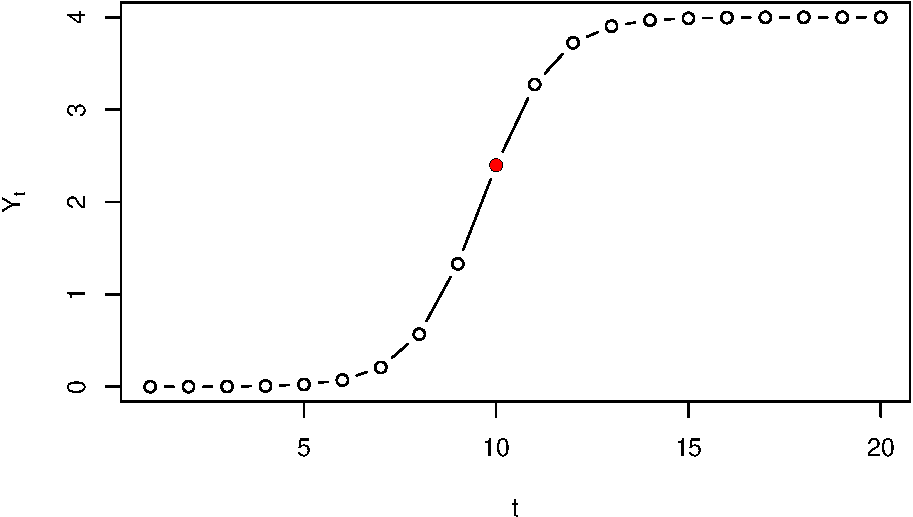
\includegraphics{DCS1617_files/figure-latex/unnamed-chunk-16-1.pdf}

\subsubsection*{Numerical solution
(discrete)}\label{numerical-solution-discrete}
\addcontentsline{toc}{subsubsection}{Numerical solution (discrete)}

If we would iterate the differential equation \ldots{}

\[
\frac{dY}{dt} = Y_t * (1 + r - r * \frac{Y_t}{K})
\]

\ldots{} as if it were a difference equation, that is, \emph{not}
simulating continuous time.

\begin{Shaded}
\begin{Highlighting}[]
\NormalTok{logIter <-}\StringTok{  }\NormalTok{function(Y0,r,K,t)\{}
  \NormalTok{N <-}\StringTok{ }\KeywordTok{length}\NormalTok{(t)}
  \NormalTok{Y <-}\StringTok{ }\KeywordTok{as.numeric}\NormalTok{(}\KeywordTok{c}\NormalTok{(Y0, }\KeywordTok{rep}\NormalTok{(}\OtherTok{NA}\NormalTok{,N}\DecValTok{-2}\NormalTok{)))}
  \KeywordTok{sapply}\NormalTok{(}\KeywordTok{seq_along}\NormalTok{(Y), function(t)\{ Y[[t}\DecValTok{+1}\NormalTok{]] <<-}\StringTok{ }\NormalTok{Y[t] *}\StringTok{ }\NormalTok{(}\DecValTok{1} \NormalTok{+}\StringTok{ }\NormalTok{r -}\StringTok{ }\NormalTok{r *}\StringTok{ }\NormalTok{Y[t] /}\StringTok{ }\NormalTok{K)\})}
  \NormalTok{\}}

\CommentTok{# Plot from t=1 to t=100}
\KeywordTok{plot}\NormalTok{(}\KeywordTok{logIter}\NormalTok{(}\DataTypeTok{Y0=}\NormalTok{.}\DecValTok{0001}\NormalTok{, }\DataTypeTok{r=}\FloatTok{1.1}\NormalTok{, }\DataTypeTok{K=}\DecValTok{4}\NormalTok{, }\DataTypeTok{t=}\KeywordTok{seq}\NormalTok{(}\DecValTok{1}\NormalTok{,}\DecValTok{20}\NormalTok{)), }\DataTypeTok{type =} \StringTok{"b"}\NormalTok{, }
     \DataTypeTok{ylab =} \KeywordTok{expression}\NormalTok{(Y[t]), }\DataTypeTok{xlab =} \StringTok{"t"}\NormalTok{)}
\CommentTok{# Plot t=10 in red}
\KeywordTok{points}\NormalTok{(}\DecValTok{10}\NormalTok{,}\KeywordTok{logSol}\NormalTok{(}\DataTypeTok{Y0=}\NormalTok{.}\DecValTok{0001}\NormalTok{, }\DataTypeTok{r=}\FloatTok{1.1}\NormalTok{, }\DataTypeTok{K=}\DecValTok{4}\NormalTok{, }\DataTypeTok{t=}\DecValTok{10}\NormalTok{), }\DataTypeTok{col=}\StringTok{"red"}\NormalTok{, }\DataTypeTok{pch=}\DecValTok{16}\NormalTok{)}
\end{Highlighting}
\end{Shaded}

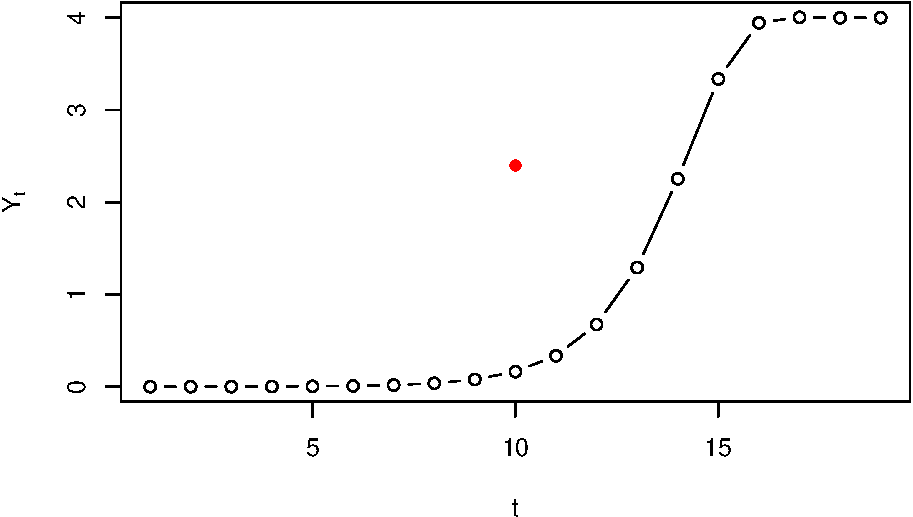
\includegraphics{DCS1617_files/figure-latex/unnamed-chunk-17-1.pdf}

\chapter*{Lecture 3}\label{lecture-3}
\addcontentsline{toc}{chapter}{Lecture 3}

\subsection*{\texorpdfstring{New to
\texttt{R}?}{New to R?}}\label{new-to-r}
\addcontentsline{toc}{subsection}{New to \texttt{R}?}

You have probably heard many people say they should invest more time and
effort to learn to use the \texttt{R} software environment for
statistical computing\ldots{} \emph{and they were right}. However, what
they probably meant to say is: ``I tried it, but it's so damned
complicated, I gave up''\ldots{} \emph{and they were right}. That is,
they were right to note that this is not a point and click tool designed
to accommodate any user. It was built for the niche market of scientists
who use statistics, but in that segment it's actually the most useful
tool I have encountered so far. Now that your struggles with getting a
grip on \texttt{R} are fully acknowledged in advance, let's try to avoid
the `giving up' from happening. Try to follow these steps to get
started:

\begin{enumerate}
\def\labelenumi{\arabic{enumi}.}
\item
  \textbf{Get \texttt{R} and add some user comfort:} Install the latest
  \href{http://www.r-project.org}{\texttt{R} software} \emph{and}
  install a user interface like
  \href{http://www.rstudio.com}{RStudio}\ldots{} \emph{It's all free!}
  An R interface will make some things easier, e.g., searching and
  installing packages from repositories. RStudio will also add
  functionality, like git/svn version control, project management and
  more, like the tools to create html pages like this one
  (\texttt{knitr} and \texttt{Rmarkdown}). Another source of user
  comfort are the \texttt{packages}. \texttt{R} comes with some basic
  packages installed, but you'll soon need to fit generalised linear
  mixture models, or visualise social networks using graph theory and
  that means you'll be searching for packages that allow you to do such
  things. A good place to start \emph{package hunting} are the
  \href{http://cran.r-project.org/web/views/}{CRAN task view} pages.
\item
  \textbf{Learn by running example \texttt{code}:} Copy the commands in
  the \texttt{code} blocks you find on this page, or any other tutorial
  or help files (e.g., Rob Kabacoff's
  \href{http://www.statmethods.net}{Quick R}). Paste them into an
  \texttt{.R} script file in the script (or, source) editor. In RStudio
  You can run code by pressing \texttt{cmd} + \texttt{enter} when the
  cursor is on a single single line, or you can run multiple lines at
  once by selecting them first. If you get stuck remember that there are
  expert \texttt{R} users who probably have answered your question
  already when it was posted on a forum. Search for example through the
  Stackoverflow site for
  \href{http://stackoverflow.com/questions/tagged/r}{questions tagged
  with \texttt{R}})
\item
  \textbf{Examine what happens\ldots{} when you tell \texttt{R} to make
  something happen:} \texttt{R} stores variables (anything from numeric
  data to functions) in an \texttt{Environment}. There are in fact many
  different environments, but we'll focus on the main workspace for the
  current \texttt{R} session. If you run the command
  \texttt{x\ \textless{}-\ 1+1}, a variable \texttt{x} will appear in
  the \texttt{Environment} with the value \texttt{2} assigned to it.
  Examining what happens in the \texttt{Environment} is not the same as
  examining the output of a statistical analysis. Output in \texttt{R}
  will appear in the \texttt{Console} window. Note that in a basic
  set-up each new \texttt{R} session starts with an empty
  \texttt{Environment}. If you need data in another session, you can
  save the entire \texttt{Environment}, or just some selected variables,
  to a file (\texttt{.RData}).
\item
  \textbf{Learn about the properties of \texttt{R} objects:} Think of
  objects as containers designed for specific content. One way to
  characterize the different objects in \texttt{R} is by how picky they
  are about the content you can assign it. There are objects that hold
  \texttt{character} and \texttt{numeric} type data, a \texttt{matrix}
  for numeric data organised in rows and columns, a \texttt{data.frame}
  is a matrix that allows different data types in columns, and least
  picky of all is the \texttt{list} object. It can carry any other
  object, you can have a \texttt{list} of which item 1 is an entire
  \texttt{data.frame} and item 2 is just a \texttt{character} vector of
  the letter \texttt{R}. The most difficult thing to master is how to
  efficiently work with these objects, how to assign values and query
  contents.
\item
  \textbf{Avoid repeating yourself:} The \texttt{R} language has some
  amazing properties that allow execution of many repetitive algorithmic
  operations using just a few lines of code at speeds up to warp 10.
  Naturally, you'll need to be at least half Vulcan to master these
  features properly and I catch myself copying code when I shouldn't on
  a daily basis. The first thing you will struggle with are the
  \texttt{apply} functions. These functions pass the contents of a
  \texttt{list} object to a function. Suppose we need to calculate the
  means of column variables in 40 different SPSS \texttt{.sav} files
  stored in the folder \texttt{DAT}. With the \texttt{foreign} package
  loaded we can execute the following commands:\\
  \texttt{data\ \textless{}-\ lapply(dir("/DAT/",pattern=".sav\$"),read.spss)}\\
  \texttt{out\ \ \textless{}-\ sapply(data,colMeans)}\\
  The first command applies read.spss to all files with a \texttt{.sav}
  extension found in the folder \texttt{/DAT}. It creates a dataframe
  for each file which are all stored as elements of the list
  \texttt{data}. The second line applies the function \texttt{colMeans}
  to each element of \texttt{data} and puts the combined results in a
  matrix with dataset ID as columns (1-40), dataset variables as rows
  and the calculated column means as cells. This is just the beginning
  of the \texttt{R} magic, wait 'till you learn how to write functions
  that can create functions.
\end{enumerate}

\begin{center}\rule{0.5\linewidth}{\linethickness}\end{center}

\hypertarget{lecture-4}{\chapter*{Lecture 4}\label{lecture-4}}
\addcontentsline{toc}{chapter}{Lecture 4}

It will become increasingly difficult to use software like Excel and
SPSS. Perhaps now is a good time to switch to \texttt{R} or
\texttt{Matlab}. We do have a spreadsheet example of Standardised
Dispersion Anaysis.

\subsection*{Using R: Install functions in
nlRtsa\_SOURCE.R}\label{using-r-install-functions-in-nlrtsa_source.r}
\addcontentsline{toc}{subsection}{Using R: Install functions in
nlRtsa\_SOURCE.R}

First, download (from blackboard) and
\texttt{source(\textquotesingle{}nlRtsa\_SOURCE.R\textquotesingle{})},
or source it directly from Github if you have package \texttt{devtools}
installed.

\begin{Shaded}
\begin{Highlighting}[]
\KeywordTok{library}\NormalTok{(devtools)}
\KeywordTok{source_url}\NormalTok{(}\StringTok{"https://raw.githubusercontent.com/FredHasselman/DCS/master/functionLib/nlRtsa_SOURCE.R"}\NormalTok{)}
\end{Highlighting}
\end{Shaded}

We need packages \texttt{signal} and \texttt{pracma} Among
\texttt{nlRtsa} functions is \texttt{in.IT()}, which will load a list of
packages and install them, but only if they are not present on your
system.

\begin{Shaded}
\begin{Highlighting}[]
\KeywordTok{in.IT}\NormalTok{(}\KeywordTok{c}\NormalTok{(}\StringTok{"signal"}\NormalTok{,}\StringTok{"pracma"}\NormalTok{))}
\end{Highlighting}
\end{Shaded}

You can of course also use \texttt{install.packages()} or the GUI.

\section*{Examples: Fast Fourier transform and Power
Spectrum}\label{examples-fast-fourier-transform-and-power-spectrum}
\addcontentsline{toc}{section}{Examples: Fast Fourier transform and
Power Spectrum}

Below is an example of a signal built from sine components (\texttt{y})
whose relative amplitudes are recovered in the powerspectrum. The
amplitudes are differently scaled sinewaves which are summed or
subtracted form one another.

\begin{Shaded}
\begin{Highlighting}[]
\CommentTok{# Sawtooth}
\NormalTok{x <-}\StringTok{ }\KeywordTok{seq}\NormalTok{(-}\FloatTok{3.2}\NormalTok{,}\FloatTok{3.2}\NormalTok{, }\DataTypeTok{length.out =} \DecValTok{256}\NormalTok{)}
\NormalTok{y <-}\StringTok{ }\DecValTok{2}\NormalTok{*}\KeywordTok{sin}\NormalTok{(}\DecValTok{10}\NormalTok{*x) -}\StringTok{ }\DecValTok{1}\NormalTok{*}\KeywordTok{sin}\NormalTok{(}\DecValTok{20}\NormalTok{*x) +}\StringTok{ }\NormalTok{(}\DecValTok{2}\NormalTok{/}\DecValTok{3}\NormalTok{)*}\KeywordTok{sin}\NormalTok{(}\DecValTok{30}\NormalTok{*x) -}\StringTok{ }\NormalTok{(}\DecValTok{1}\NormalTok{/}\DecValTok{2}\NormalTok{)*}\KeywordTok{sin}\NormalTok{(}\DecValTok{40}\NormalTok{*x) +}\StringTok{ }\NormalTok{(}\DecValTok{2}\NormalTok{/}\DecValTok{5}\NormalTok{)*}\KeywordTok{sin}\NormalTok{(}\DecValTok{50}\NormalTok{*x) -}\StringTok{ }\NormalTok{(}\DecValTok{1}\NormalTok{/}\DecValTok{4}\NormalTok{)*}\KeywordTok{sin}\NormalTok{(}\DecValTok{60}\NormalTok{*x)}

\CommentTok{# Plot the sawtooth wave as constructed by the Fourier series above}
\KeywordTok{plot}\NormalTok{(x,y, }\DataTypeTok{xlab =}\StringTok{'Time (a.u.)'}\NormalTok{, }\DataTypeTok{ylab =} \StringTok{'Variable (a.u.)'}\NormalTok{, }\DataTypeTok{main =}\StringTok{'Sawtooth wave'}\NormalTok{, }\DataTypeTok{type =} \StringTok{"l"}\NormalTok{)}
\end{Highlighting}
\end{Shaded}

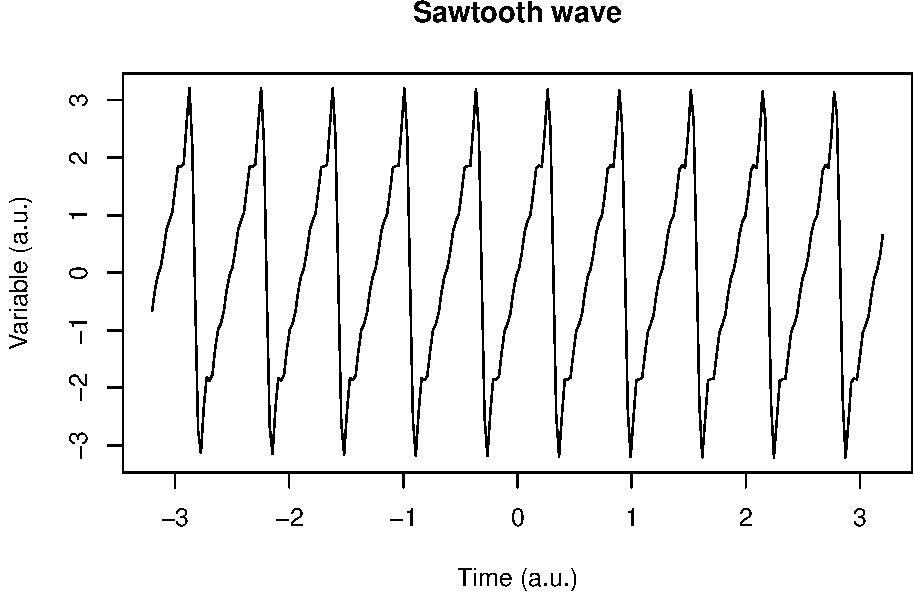
\includegraphics{DCS1617_files/figure-latex/L4.3-1.pdf}

\begin{Shaded}
\begin{Highlighting}[]
\CommentTok{# Perform a Fast Fourier Transform and calculate the Power and Frequency (you don't have to know how this works)}
\NormalTok{Y   <-}\StringTok{ }\KeywordTok{fft}\NormalTok{(y)}
\NormalTok{Pyy <-}\StringTok{ }\NormalTok{Y*}\KeywordTok{Conj}\NormalTok{(Y)/}\DecValTok{256}
\NormalTok{f <-}\StringTok{ }\DecValTok{1000}\NormalTok{/}\DecValTok{256}\NormalTok{*(}\DecValTok{0}\NormalTok{:}\DecValTok{127}\NormalTok{)}

\CommentTok{# Plot the power spectrum of the sawtooth wave}
\KeywordTok{plot}\NormalTok{(f[}\DecValTok{1}\NormalTok{:}\DecValTok{50}\NormalTok{],Pyy[}\DecValTok{1}\NormalTok{:}\DecValTok{50}\NormalTok{], }\DataTypeTok{type=}\StringTok{"b"}\NormalTok{,}\DataTypeTok{xlab=}\StringTok{'Frequency (a.u.)'}\NormalTok{, }\DataTypeTok{ylab =}\StringTok{'Power (a.u.)'}\NormalTok{, }\DataTypeTok{pch=}\DecValTok{21}\NormalTok{, }\DataTypeTok{bg=}\StringTok{'grey60'}\NormalTok{, }\DataTypeTok{main =} \StringTok{'Power Spectrum'}\NormalTok{)}
\end{Highlighting}
\end{Shaded}

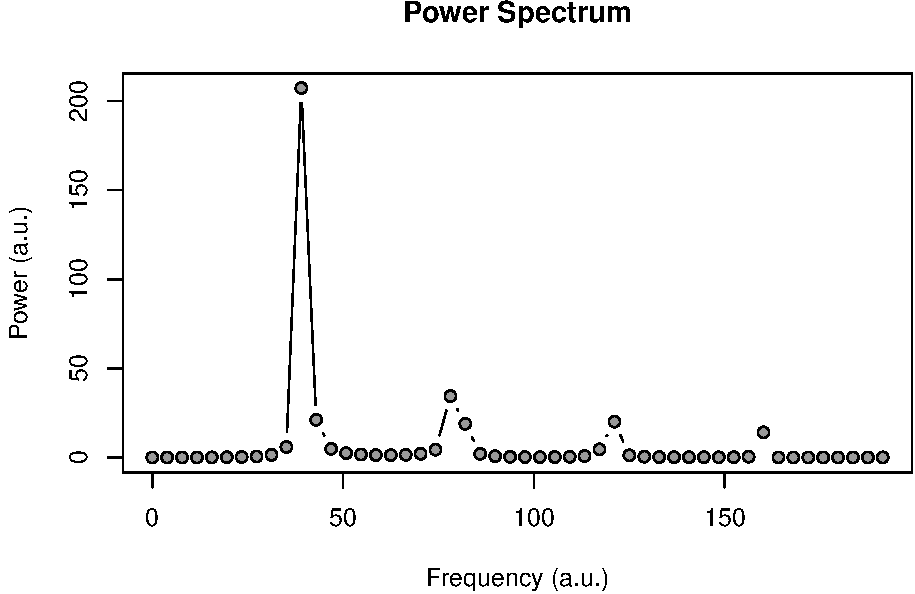
\includegraphics{DCS1617_files/figure-latex/L4.3-2.pdf}

\begin{itemize}
\tightlist
\item
  The \(6\) peaks with an amplitude \textgreater{} \(0\) are the \(6\)
  sine components used to construct the signal:
\end{itemize}

\begin{Shaded}
\begin{Highlighting}[]
\NormalTok{+}\StringTok{   }\DecValTok{2}  \NormalTok{*}\KeywordTok{sin}\NormalTok{(}\DecValTok{10}\NormalTok{*x) }
\NormalTok{-}\StringTok{   }\DecValTok{1}  \NormalTok{*}\KeywordTok{sin}\NormalTok{(}\DecValTok{20}\NormalTok{*x) }
\NormalTok{+}\StringTok{ }\NormalTok{(}\DecValTok{2}\NormalTok{/}\DecValTok{3}\NormalTok{)*}\KeywordTok{sin}\NormalTok{(}\DecValTok{30}\NormalTok{*x) }
\NormalTok{-}\StringTok{ }\NormalTok{(}\DecValTok{1}\NormalTok{/}\DecValTok{2}\NormalTok{)*}\KeywordTok{sin}\NormalTok{(}\DecValTok{40}\NormalTok{*x) }
\NormalTok{+}\StringTok{ }\NormalTok{(}\DecValTok{2}\NormalTok{/}\DecValTok{5}\NormalTok{)*}\KeywordTok{sin}\NormalTok{(}\DecValTok{50}\NormalTok{*x) }
\NormalTok{-}\StringTok{ }\NormalTok{(}\DecValTok{1}\NormalTok{/}\DecValTok{4}\NormalTok{)*}\KeywordTok{sin}\NormalTok{(}\DecValTok{60}\NormalTok{*x)}
\end{Highlighting}
\end{Shaded}

Now we do the same for a very noisy signal into which we insert one
dominant frequency and two smaller ones.

\begin{Shaded}
\begin{Highlighting}[]
\CommentTok{# A time vector}
\NormalTok{t <-}\StringTok{ }\NormalTok{pracma::}\KeywordTok{linspace}\NormalTok{(}\DataTypeTok{x1 =} \DecValTok{0}\NormalTok{, }\DataTypeTok{x2 =} \DecValTok{50}\NormalTok{, }\DataTypeTok{n =} \DecValTok{256}\NormalTok{)}
\CommentTok{# There are three sine components}
\NormalTok{x <-}\StringTok{ }\KeywordTok{sin}\NormalTok{(}\DecValTok{2}\NormalTok{*pi*t/.}\DecValTok{1}\NormalTok{) +}\StringTok{ }\KeywordTok{sin}\NormalTok{(}\DecValTok{2}\NormalTok{*pi*t/.}\DecValTok{3}\NormalTok{) +}\StringTok{ }\KeywordTok{sin}\NormalTok{(}\DecValTok{2}\NormalTok{*pi*t/.}\DecValTok{5}\NormalTok{)}
\CommentTok{# Add random noise!}
\NormalTok{y <-}\StringTok{ }\NormalTok{x +}\StringTok{ }\DecValTok{1}\NormalTok{*}\KeywordTok{randn}\NormalTok{(}\KeywordTok{size}\NormalTok{(t))}

\CommentTok{# Plot the noise.}
\KeywordTok{plot}\NormalTok{(t, y, }\DataTypeTok{type =} \StringTok{"l"}\NormalTok{, }\DataTypeTok{xlab =} \StringTok{'Time (a.u.)'}\NormalTok{, }\DataTypeTok{ylab =} \StringTok{'Variable (a.u.)'}\NormalTok{, }\DataTypeTok{main =} \StringTok{'A very noisy signal'}\NormalTok{)}
\end{Highlighting}
\end{Shaded}

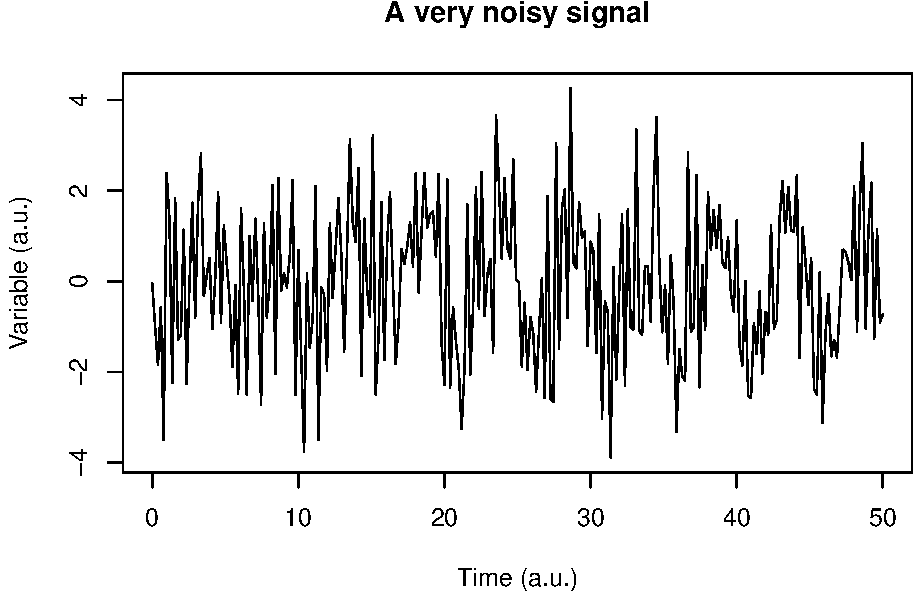
\includegraphics{DCS1617_files/figure-latex/L4.5-1.pdf}

\begin{Shaded}
\begin{Highlighting}[]
\CommentTok{# Get the frequency domain}
\NormalTok{Y <-}\StringTok{ }\KeywordTok{fft}\NormalTok{(y)}
\NormalTok{Pyy <-}\StringTok{ }\NormalTok{Y*}\KeywordTok{Conj}\NormalTok{(Y)/}\DecValTok{256}
\NormalTok{f <-}\StringTok{ }\DecValTok{1000}\NormalTok{/}\DecValTok{256}\NormalTok{*(}\DecValTok{0}\NormalTok{:}\DecValTok{127}\NormalTok{)}

\CommentTok{# Plot the power spectrum of this noise}
\KeywordTok{plot}\NormalTok{(f[}\DecValTok{1}\NormalTok{:}\DecValTok{50}\NormalTok{],Pyy[}\DecValTok{1}\NormalTok{:}\DecValTok{50}\NormalTok{], }\DataTypeTok{type=}\StringTok{"b"}\NormalTok{,}\DataTypeTok{xlab=}\StringTok{'Frequency (a.u.)'}\NormalTok{, }\DataTypeTok{ylab=}\StringTok{'Power (a.u.)'}\NormalTok{, }\DataTypeTok{pch=}\DecValTok{21}\NormalTok{, }\DataTypeTok{bg=}\StringTok{'grey60'}\NormalTok{, }\DataTypeTok{main =} \StringTok{'Power Spectrum'}\NormalTok{)}
\end{Highlighting}
\end{Shaded}

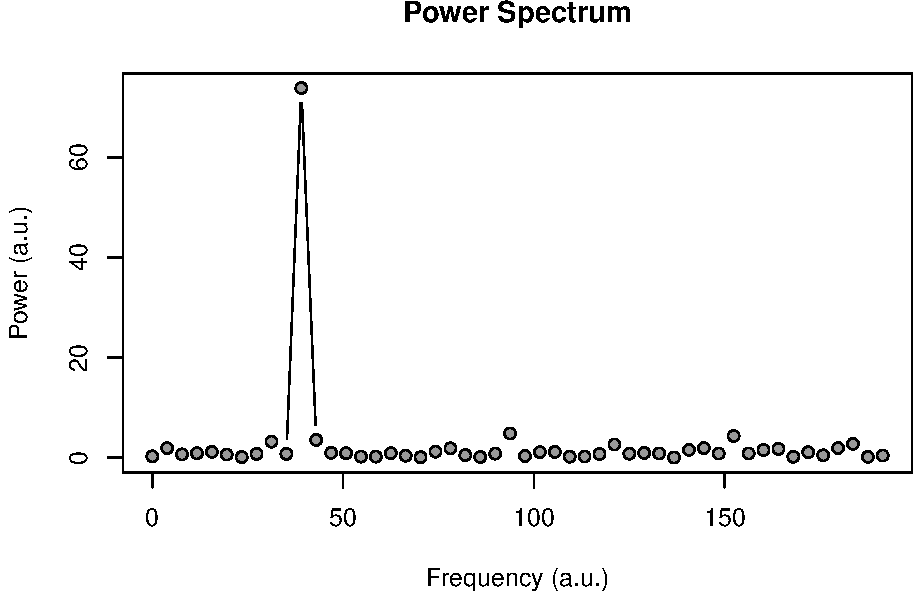
\includegraphics{DCS1617_files/figure-latex/L4.5-2.pdf}

\begin{itemize}
\tightlist
\item
  The \(3\) peaks with an amplitude \textgreater{} \(0\) are the \(3\)
  sine components used to construct the signal to which random noise was
  added:
\end{itemize}

\begin{Shaded}
\begin{Highlighting}[]
\NormalTok{+}\StringTok{ }\KeywordTok{sin}\NormalTok{(}\DecValTok{2}\NormalTok{*pi*t/.}\DecValTok{1}\NormalTok{) }
\NormalTok{+}\StringTok{ }\KeywordTok{sin}\NormalTok{(}\DecValTok{2}\NormalTok{*pi*t/.}\DecValTok{3}\NormalTok{) }
\NormalTok{+}\StringTok{ }\KeywordTok{sin}\NormalTok{(}\DecValTok{2}\NormalTok{*pi*t/.}\DecValTok{5}\NormalTok{)}
\end{Highlighting}
\end{Shaded}

More information about the
\href{https://en.wikipedia.org/wiki/Fourier_transform}{Fourier
transform} and
\href{http://www.di.fc.ul.pt/~jpn/r/fourier/fourier.html}{how to use
\texttt{R} functions}.

\hypertarget{data-considerations}{\section*{Data
considerations}\label{data-considerations}}
\addcontentsline{toc}{section}{Data considerations}

\begin{quote}
``If you have not found the fractal pattern, you have not taken enough
data'' -- Machlup, 1977)
\end{quote}

\begin{itemize}
\tightlist
\item
  \textbf{All analyses}:

  \begin{itemize}
  \tightlist
  \item
    Data points: \(2^n\), minimum 1024 (\(2^{10}\))
  \item
    Remove 3SD only if this is absolutely necessary
  \end{itemize}
\item
  \textbf{Spectral analysis}:

  \begin{itemize}
  \tightlist
  \item
    Normalize the data (z-score transform: (X-mean(X))/SD(X)
  \item
    Remove linear trend if necessary (detrend)
  \item
    Decide number of frequencies to estimate, min. 512
  \end{itemize}
\item
  \textbf{SDA}:

  \begin{itemize}
  \tightlist
  \item
    Normalize the data (z-score transform: (X-mean(X))/SD(X)
  \end{itemize}
\item
  \textbf{DFA}:

  \begin{itemize}
  \tightlist
  \item
    Nothing extra, analysis integrates and detrends the signal
  \end{itemize}
\end{itemize}

\chapter*{Lecture 5}\label{lecture-5}
\addcontentsline{toc}{chapter}{Lecture 5}

\chapter*{Lecture 6}\label{lecture-6}
\addcontentsline{toc}{chapter}{Lecture 6}

\chapter*{Lecture 7}\label{lecture-7}
\addcontentsline{toc}{chapter}{Lecture 7}

\chapter*{Lecture 8}\label{lecture-8}
\addcontentsline{toc}{chapter}{Lecture 8}

\chapter*{Lecture 9}\label{lecture-9}
\addcontentsline{toc}{chapter}{Lecture 9}

\appendix


\chapter{\texorpdfstring{\textbf{Mathematics of change
I}}{Mathematics of change I}}\label{mathematics-of-change-i}

Solutions to assignments in section \ref{moc1ass}.

\begin{itemize}
\tightlist
\item
  Linear and logistic growth
\item
  Deterministic Chaos
\end{itemize}

\hypertarget{linear-and-logistic-growth}{\section{Linear and logistic
growth}\label{linear-and-logistic-growth}}

\subsection*{Solutions in a
spreadsheet}\label{solutions-in-a-spreadsheet}
\addcontentsline{toc}{subsection}{Solutions in a spreadsheet}

The solutions to iterating the Linear Map and theLogistic Map in a
spreadsheet can be found in this
\href{https://docs.google.com/spreadsheets/d/1BL_oKoCFH3NQ3qKLBQ-WbkPg_ppSZsyDNl2nS9oPGcM/edit?usp=sharing}{GoogleSheet}.

\subsection*{\texorpdfstring{Solutions in
\texttt{R}}{Solutions in R}}\label{solutions-in-r}
\addcontentsline{toc}{subsection}{Solutions in \texttt{R}}

\href{\%7B\#moc1R\%7D}{\textbar{} jump to question \textbar{}}

Coding the difference equations in \texttt{Matlab} and \texttt{R} is
always easier than using a spreadsheet. One obvious way to do it is to
use a counter variable representing the iterations of time in a
\texttt{for\ ...\ next} loop. The iterations should run over a vector
(which is the same concept as a row or a column in a spreadsheet: An
indexed array of numbers or characters). The first entry should be the
starting value, so the vector index \(1\) represents \(Y_0\).

The loop can be implemented a number of ways, for example as a function
which can be called from a script or the command / console window. In
\texttt{R} working with functions is easy, and very much recommended,
because it will speed up calculations considerably, and it will reduce
the amount of code you need to write. You need to gain some experience
with coding in \texttt{R} before you'll get it right. In order to get it
lean and clean (and possibly even mean as well) you'll need a lot of
experience with coding in \texttt{R},therefore, we will (eventually)
provide you the functions you'll need to complete the assignments. All
you have to do is figure out how to use, or modify them to suit your
specific needs.

To model the autocatalytic growth equations we provide a function
\texttt{growth.ac()}, which is able to simulate all of the processes
discussed in the lectures. Using just a few lines of code, each of the 4
difference equations used in the assignments can be simulated. Basically
the code block below contains the solutions to the Linear Map, the
stylized Logisitc Map and the Van Geert model for cognitive growth.

\begin{Shaded}
\begin{Highlighting}[]
\NormalTok{growth.ac <-}\StringTok{ }\NormalTok{function(}\DataTypeTok{Y0 =} \FloatTok{0.01}\NormalTok{, }\DataTypeTok{r =} \DecValTok{1}\NormalTok{, }\DataTypeTok{k =} \DecValTok{1}\NormalTok{, }\DataTypeTok{N =} \DecValTok{100}\NormalTok{, }\DataTypeTok{type =} \KeywordTok{c}\NormalTok{(}\StringTok{"driving"}\NormalTok{, }\StringTok{"damping"}\NormalTok{, }\StringTok{"logistic"}\NormalTok{, }\StringTok{"vanGeert"}\NormalTok{)[}\DecValTok{1}\NormalTok{])\{}
    \CommentTok{# Create a vector Y of length N, which has value Y0 at Y[1]}
    \NormalTok{if(N>}\DecValTok{1}\NormalTok{)\{}
    \NormalTok{Y <-}\StringTok{ }\KeywordTok{as.numeric}\NormalTok{(}\KeywordTok{c}\NormalTok{(Y0, }\KeywordTok{rep}\NormalTok{(}\OtherTok{NA}\NormalTok{,N}\DecValTok{-2}\NormalTok{)))}
    \CommentTok{# Conditional on the value of type ... }
    \NormalTok{switch(type, }
           \CommentTok{# Iterate N steps of the difference function with values passed for Y0, k and r.}
           \DataTypeTok{driving  =} \KeywordTok{sapply}\NormalTok{(}\KeywordTok{seq_along}\NormalTok{(Y), function(t) Y[[t}\DecValTok{+1}\NormalTok{]] <<-}\StringTok{ }\NormalTok{r *}\StringTok{ }\NormalTok{Y[t] ),}
           \DataTypeTok{damping  =} \NormalTok{k +}\StringTok{ }\KeywordTok{sapply}\NormalTok{(}\KeywordTok{seq_along}\NormalTok{(Y), function(t) Y[[t}\DecValTok{+1}\NormalTok{]] <<-}\StringTok{ }\NormalTok{-}\StringTok{ }\NormalTok{r *}\StringTok{ }\NormalTok{Y[t]^}\DecValTok{2} \NormalTok{/}\StringTok{ }\NormalTok{k),}
           \DataTypeTok{logistic =} \KeywordTok{sapply}\NormalTok{(}\KeywordTok{seq_along}\NormalTok{(Y), function(t) Y[[t}\DecValTok{+1}\NormalTok{]] <<-}\StringTok{ }\NormalTok{r *}\StringTok{ }\NormalTok{Y[t] *}\StringTok{ }\NormalTok{((k -}\StringTok{ }\NormalTok{Y[t]) /}\StringTok{ }\NormalTok{k)),}
           \DataTypeTok{vanGeert =} \KeywordTok{sapply}\NormalTok{(}\KeywordTok{seq_along}\NormalTok{(Y), function(t) Y[[t}\DecValTok{+1}\NormalTok{]] <<-}\StringTok{ }\NormalTok{Y[t] *}\StringTok{ }\NormalTok{(}\DecValTok{1} \NormalTok{+}\StringTok{ }\NormalTok{r -}\StringTok{ }\NormalTok{r *}\StringTok{ }\NormalTok{Y[t] /}\StringTok{ }\NormalTok{k)) }
    \NormalTok{)\}}
    \KeywordTok{return}\NormalTok{(}\KeywordTok{ts}\NormalTok{(Y))}
\NormalTok{\}}

\CommentTok{# Call the function with default settings and r = 1.1}
\NormalTok{Y <-}\StringTok{ }\KeywordTok{growth.ac}\NormalTok{(}\DataTypeTok{r =} \FloatTok{1.1}\NormalTok{)}
\end{Highlighting}
\end{Shaded}

Some notes about this function:

\begin{itemize}
\tightlist
\item
  To select which growth process to simulate, the argument \texttt{type}
  is defined which takes the values \texttt{driving} (default),
  \texttt{damping}, \texttt{logistic} and \texttt{vanGeert}.

  \begin{itemize}
  \tightlist
  \item
    The statement \texttt{switch(type,\ ...)} will iterate an equation
    based on the value of \texttt{type}.
  \end{itemize}
\item
  A \texttt{time\ series} object is returned due to the function
  \texttt{ts()}. This is a convenient way to represent time series data,
  it can also store the sample rate of the signal and start and end
  times.

  \begin{itemize}
  \tightlist
  \item
    Most of the basic functions, like \texttt{plot()} and
    \texttt{summary()} will recognise a time series object when it is
    passed as an argument and use settings appropriate for time series
    data.
  \end{itemize}
\item
  The \texttt{sapply()} function iterates \(t\) from \(1\) to the number
  of elements in \(Y\) (\texttt{seq\_along(Y)}) and then applies the
  function.
\item
  The double headed arrow \texttt{\textless{}\textless{}-} is necessary
  because we want to update vector \(Y\), which is defined outside the
  \texttt{sapply()} environment.
\end{itemize}

\subsubsection*{\texorpdfstring{The \texttt{time\ series}
object}{The time series object}}\label{the-time-series-object}
\addcontentsline{toc}{subsubsection}{The \texttt{time\ series} object}

The time series object is expected to have a time-dimension on the
x-axis. This is very convenient, because \texttt{R} will generate the
time axis for you by looking at the \emph{t}ime \emph{s}eries
\emph{p}roperties attribute of the object. Even though we are not
working with measurement ourcomes, consider a value at a time-index in a
time series object a \textbf{sample}:

\begin{itemize}
\tightlist
\item
  \texttt{Start} - The value of time at the first sample in the series
  (e.g., \(0\), or \(1905\))
\item
  \texttt{End} - The value of time at the last sample in the series
  (e.g., \(100\), or \(2005\))
\item
  \texttt{Frequency} - The amount of time that passed between two
  samples, or, the sample rate (e.g., \(0.5\), or \(10\))
\end{itemize}

Examples of using the time series object.

\begin{Shaded}
\begin{Highlighting}[]
\CommentTok{# Get sample rate info}
\KeywordTok{tsp}\NormalTok{(Y)}
\end{Highlighting}
\end{Shaded}

\begin{verbatim}
[1]   1 100   1
\end{verbatim}

\begin{Shaded}
\begin{Highlighting}[]
\CommentTok{# Extract the time vector}
\KeywordTok{time}\NormalTok{(Y)}
\end{Highlighting}
\end{Shaded}

\begin{verbatim}
Time Series:
Start = 1 
End = 100 
Frequency = 1 
  [1]   1   2   3   4   5   6   7   8   9  10  11  12  13  14  15  16  17
 [18]  18  19  20  21  22  23  24  25  26  27  28  29  30  31  32  33  34
 [35]  35  36  37  38  39  40  41  42  43  44  45  46  47  48  49  50  51
 [52]  52  53  54  55  56  57  58  59  60  61  62  63  64  65  66  67  68
 [69]  69  70  71  72  73  74  75  76  77  78  79  80  81  82  83  84  85
 [86]  86  87  88  89  90  91  92  93  94  95  96  97  98  99 100
\end{verbatim}

For now, these values are in principle all arbitrary units
(\texttt{a.u.}). These settings only make sense if they represent the
parameters of an actual measurement procedure.

It is easy to adjust the time vector, by assigning new values using
\texttt{tsp()} (values have to be possible given the timeseries length).
For example, suppose the sampling frequency was \(0.1\) instead of \(1\)
and the Start time was \(10\) and End time was \(1000\).

\begin{Shaded}
\begin{Highlighting}[]
\CommentTok{# Assign new values}
\KeywordTok{tsp}\NormalTok{(Y) <-}\StringTok{ }\KeywordTok{c}\NormalTok{(}\DecValTok{10}\NormalTok{, }\DecValTok{1000}\NormalTok{, .}\DecValTok{1}\NormalTok{)}
\CommentTok{# Time axis is automatically adjusted }
\KeywordTok{time}\NormalTok{(Y)}
\end{Highlighting}
\end{Shaded}

\begin{verbatim}
Time Series:
Start = 10 
End = 1000 
Frequency = 0.1 
  [1]   10   20   30   40   50   60   70   80   90  100  110  120  130  140
 [15]  150  160  170  180  190  200  210  220  230  240  250  260  270  280
 [29]  290  300  310  320  330  340  350  360  370  380  390  400  410  420
 [43]  430  440  450  460  470  480  490  500  510  520  530  540  550  560
 [57]  570  580  590  600  610  620  630  640  650  660  670  680  690  700
 [71]  710  720  730  740  750  760  770  780  790  800  810  820  830  840
 [85]  850  860  870  880  890  900  910  920  930  940  950  960  970  980
 [99]  990 1000
\end{verbatim}

\subsubsection*{\texorpdfstring{Plotting a \texttt{ts} object as a time
series}{Plotting a ts object as a time series}}\label{plotting-a-ts-object-as-a-time-series}
\addcontentsline{toc}{subsubsection}{Plotting a \texttt{ts} object as a
time series}

Depending on which packages you use, there will be different settings
applied to time series objects created by \texttt{ts()}. Below are some
examples of differences between plotting routines.

\begin{Shaded}
\begin{Highlighting}[]
\KeywordTok{require}\NormalTok{(lattice)       }\CommentTok{# Needed for plotting}
\KeywordTok{require}\NormalTok{(latticeExtra)  }\CommentTok{# Needed for plotting}

\CommentTok{# stats::plot.ts}
\KeywordTok{plot}\NormalTok{(}\KeywordTok{growth.ac}\NormalTok{(}\DataTypeTok{r =} \NormalTok{-.}\DecValTok{9}\NormalTok{), }\DataTypeTok{lwd =} \DecValTok{2}\NormalTok{, }\DataTypeTok{main =} \StringTok{"stats::plot.ts"}\NormalTok{)}
\end{Highlighting}
\end{Shaded}

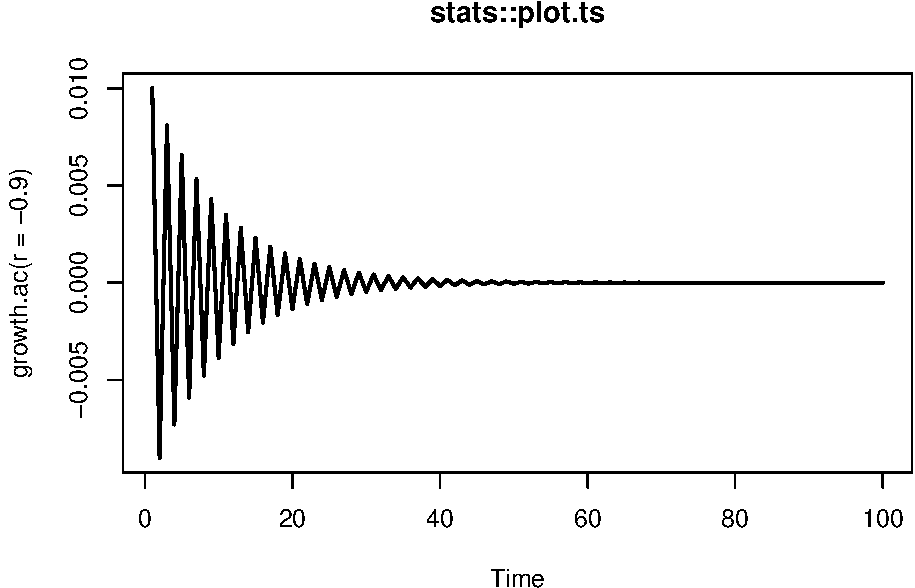
\includegraphics{DCS1617_files/figure-latex/unnamed-chunk-24-1.pdf}

\begin{Shaded}
\begin{Highlighting}[]
\CommentTok{# lattice::xyplot.ts}
\KeywordTok{xyplot}\NormalTok{(}\KeywordTok{growth.ac}\NormalTok{(}\DataTypeTok{r =} \NormalTok{-.}\DecValTok{9}\NormalTok{), }\DataTypeTok{lwd =} \DecValTok{2}\NormalTok{, }\DataTypeTok{main =} \StringTok{"lattice::xyplot.ts"}\NormalTok{)}
\end{Highlighting}
\end{Shaded}

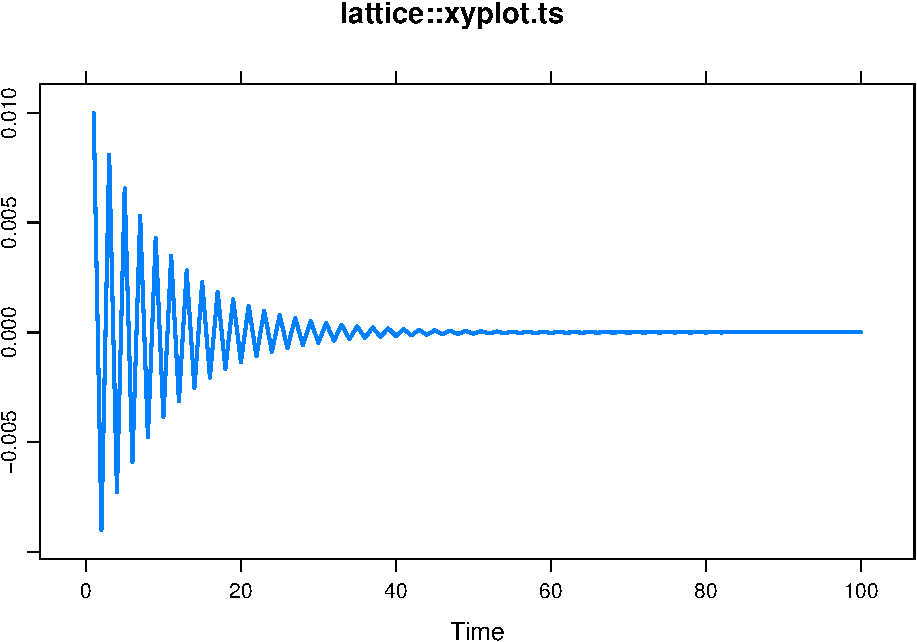
\includegraphics{DCS1617_files/figure-latex/unnamed-chunk-24-2.pdf}

\subsubsection*{Plotting multiple time series in one
figure}\label{plotting-multiple-time-series-in-one-figure}
\addcontentsline{toc}{subsubsection}{Plotting multiple time series in
one figure}

Plot multiple timeseries in frames with \texttt{plot.ts()} in
\texttt{package::stats}. This function takes a matrix as input, here we
use \texttt{cbind(\ ...\ )}.

\begin{Shaded}
\begin{Highlighting}[]
\CommentTok{# stats::plot.ts  }
\KeywordTok{plot}\NormalTok{(}\KeywordTok{cbind}\NormalTok{(}\KeywordTok{growth.ac}\NormalTok{(}\DataTypeTok{r =}  \FloatTok{0.9}\NormalTok{),}
           \KeywordTok{growth.ac}\NormalTok{(}\DataTypeTok{r =}  \FloatTok{1.0}\NormalTok{), }
           \KeywordTok{growth.ac}\NormalTok{(}\DataTypeTok{r =} \NormalTok{-}\FloatTok{0.8}\NormalTok{)}
           \NormalTok{), }
     \DataTypeTok{yax.flip =} \OtherTok{TRUE}\NormalTok{, }\DataTypeTok{ann =} \OtherTok{FALSE}\NormalTok{, }\DataTypeTok{col =} \StringTok{"blue"}\NormalTok{, }\DataTypeTok{frame.plot =} \OtherTok{TRUE}\NormalTok{) }
\KeywordTok{title}\NormalTok{(}\DataTypeTok{main =} \KeywordTok{expression}\NormalTok{(}\KeywordTok{paste}\NormalTok{(}\StringTok{"Unrestricted Growth: "}\NormalTok{,Y[t}\DecValTok{+1}\NormalTok{]==r*Y[t])), }
      \DataTypeTok{ylab =} \StringTok{"|  r = -0.8  |  r = 1  |  r = 0.9  |"}\NormalTok{, }
      \DataTypeTok{xlab =} \StringTok{"time (a.u.)"}\NormalTok{)}
\end{Highlighting}
\end{Shaded}

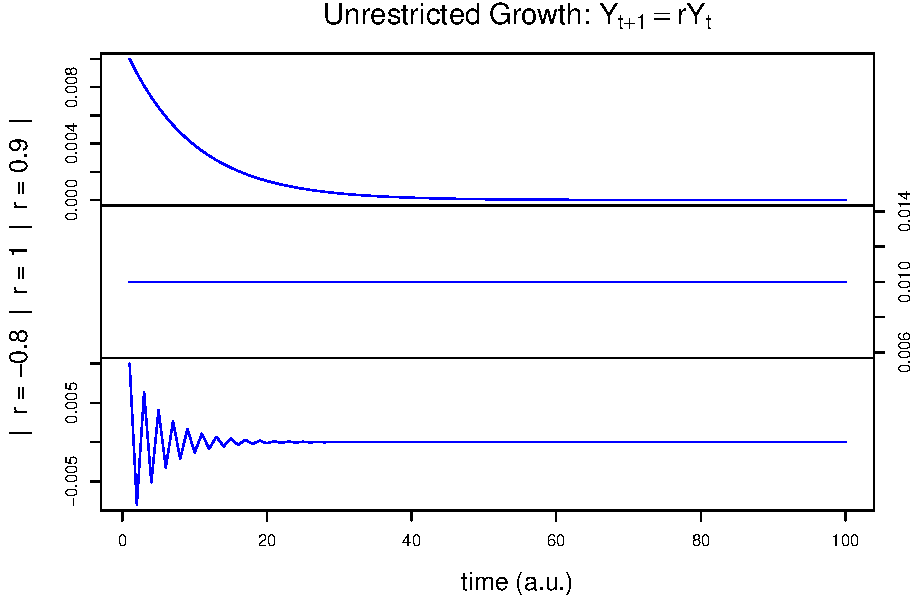
\includegraphics{DCS1617_files/figure-latex/unnamed-chunk-25-1.pdf}

Plot multiple timeseries in one graph with \texttt{ts.plot()} in
\texttt{package::graphics}. This function can handle multiple
\texttt{ts} objects as arguments.

\begin{Shaded}
\begin{Highlighting}[]
\CommentTok{# graphics::ts.plot}
\KeywordTok{ts.plot}\NormalTok{(}\KeywordTok{growth.ac}\NormalTok{(}\DataTypeTok{r =} \FloatTok{0.9}\NormalTok{), }
        \KeywordTok{growth.ac}\NormalTok{(}\DataTypeTok{r =} \DecValTok{1}\NormalTok{), }
        \KeywordTok{growth.ac}\NormalTok{(}\DataTypeTok{r =} \NormalTok{-.}\DecValTok{8}\NormalTok{), }
        \DataTypeTok{gpars =} \KeywordTok{list}\NormalTok{(}\DataTypeTok{xlab =} \StringTok{"time (a.u.)"}\NormalTok{,}
                     \DataTypeTok{ylab =} \KeywordTok{expression}\NormalTok{(}\KeywordTok{Y}\NormalTok{(t)),}
                     \DataTypeTok{main =} \KeywordTok{expression}\NormalTok{(}\KeywordTok{paste}\NormalTok{(}\StringTok{"Unrestricted Growth: "}\NormalTok{,Y[t}\DecValTok{+1}\NormalTok{]==r*Y[t])),}
                     \DataTypeTok{lwd =} \KeywordTok{rep}\NormalTok{(}\DecValTok{2}\NormalTok{,}\DecValTok{3}\NormalTok{),}
                     \DataTypeTok{lty =} \KeywordTok{c}\NormalTok{(}\DecValTok{1}\NormalTok{:}\DecValTok{3}\NormalTok{),}
                     \DataTypeTok{col =} \KeywordTok{c}\NormalTok{(}\StringTok{"darkred"}\NormalTok{,}\StringTok{"darkblue"}\NormalTok{,}\StringTok{"darkgreen"}\NormalTok{)}
                     \NormalTok{)}
        \NormalTok{)}
\KeywordTok{legend}\NormalTok{(}\DecValTok{70}\NormalTok{, -}\FloatTok{0.015}\NormalTok{, }\KeywordTok{c}\NormalTok{(}\StringTok{"r = 0.9"}\NormalTok{,}\StringTok{"r = 1.0"}\NormalTok{, }\StringTok{"r = -0.8"}\NormalTok{), }\DataTypeTok{lwd =} \KeywordTok{rep}\NormalTok{(}\DecValTok{2}\NormalTok{,}\DecValTok{3}\NormalTok{), }\DataTypeTok{lty =} \KeywordTok{c}\NormalTok{(}\DecValTok{1}\NormalTok{:}\DecValTok{3}\NormalTok{), }\DataTypeTok{col =} \KeywordTok{c}\NormalTok{(}\StringTok{"darkred"}\NormalTok{,}\StringTok{"darkblue"}\NormalTok{,}\StringTok{"darkgreen"}\NormalTok{), }\DataTypeTok{merge =} \OtherTok{TRUE}\NormalTok{)}
\end{Highlighting}
\end{Shaded}

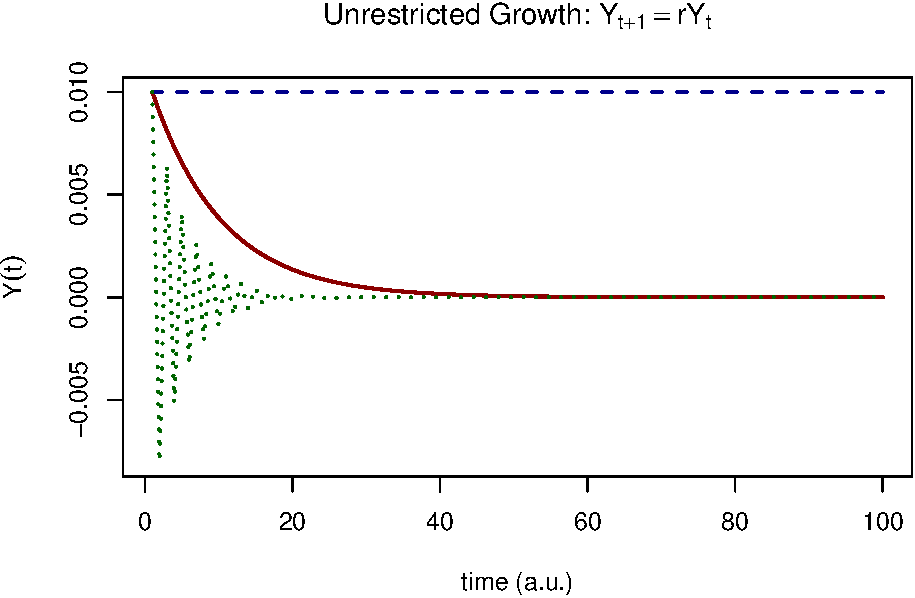
\includegraphics{DCS1617_files/figure-latex/unnamed-chunk-26-1.pdf}

Use \texttt{xyplot()} in \texttt{package::lattice} to create a plot with
panels. The easiest way to do this is to create a dataset in so-called
``long'' format. This means the variable to plot is in 1 column and
other variables indicate different levels, or conditions under which the
variable was observed or simulated.

Function \texttt{ldply()} is used to generate \(Y\) for three different
settings of \(r\). The values of \(r\) are passed as a \textbf{l}ist and
after a function is applied the result is returned as a
\textbf{d}ataframe.

\begin{Shaded}
\begin{Highlighting}[]
\KeywordTok{require}\NormalTok{(plyr)          }\CommentTok{# Needed for function ldply()}

\CommentTok{# Create a long format dataframe for various values for `r`}
\NormalTok{data <-}\StringTok{ }\KeywordTok{ldply}\NormalTok{(}\KeywordTok{c}\NormalTok{(}\FloatTok{0.9}\NormalTok{,}\DecValTok{1}\NormalTok{,-}\FloatTok{0.8}\NormalTok{), function(r) }\KeywordTok{cbind.data.frame}\NormalTok{(}\DataTypeTok{Y    =} \KeywordTok{as.numeric}\NormalTok{(}\KeywordTok{growth.ac}\NormalTok{(}\DataTypeTok{r =} \NormalTok{r)),}
                                                          \DataTypeTok{time =} \KeywordTok{as.numeric}\NormalTok{(}\KeywordTok{time}\NormalTok{(}\KeywordTok{growth.ac}\NormalTok{(}\DataTypeTok{r =} \NormalTok{r))),}
                                                          \DataTypeTok{r    =} \KeywordTok{paste0}\NormalTok{(}\StringTok{"r = "}\NormalTok{, r)))}
\CommentTok{# Plot using the formula interface}
\KeywordTok{xyplot}\NormalTok{(Y ~}\StringTok{ }\NormalTok{time |}\StringTok{ }\NormalTok{r, }\DataTypeTok{data =} \NormalTok{data, }\DataTypeTok{type =} \StringTok{"l"}\NormalTok{, }\DataTypeTok{main =} \KeywordTok{expression}\NormalTok{(}\KeywordTok{paste}\NormalTok{(}\StringTok{"Unrestricted Growth: "}\NormalTok{,Y[t}\DecValTok{+1}\NormalTok{]==r*Y[t])))}
\end{Highlighting}
\end{Shaded}

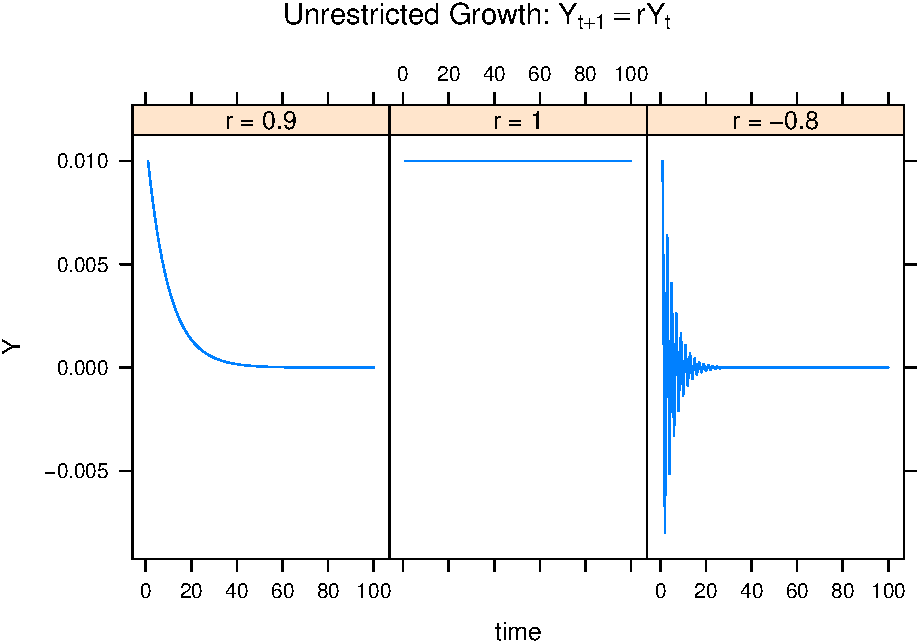
\includegraphics{DCS1617_files/figure-latex/unnamed-chunk-27-1.pdf}

One can also have different panels represent different growth functions.

\begin{Shaded}
\begin{Highlighting}[]
\CommentTok{# Create a long format dataframe for combinations of `type` and `r`}
\NormalTok{param <-}\StringTok{ }\KeywordTok{list}\NormalTok{(}\DataTypeTok{driving  =} \FloatTok{1.1}\NormalTok{,}
              \DataTypeTok{damping  =} \FloatTok{0.9}\NormalTok{,}
              \DataTypeTok{logistic =} \FloatTok{2.9}\NormalTok{,}
              \DataTypeTok{vanGeert =} \FloatTok{1.9}\NormalTok{)}
\CommentTok{# Use the `names()` function to pass the `type` string as an argument.}
\NormalTok{data <-}\StringTok{ }\KeywordTok{ldply}\NormalTok{(}\KeywordTok{seq_along}\NormalTok{(param), function(p)\{}
    \KeywordTok{cbind.data.frame}\NormalTok{(}\DataTypeTok{Y    =} \KeywordTok{as.numeric}\NormalTok{(}\KeywordTok{growth.ac}\NormalTok{(}\DataTypeTok{r =} \NormalTok{param[[p]], }\DataTypeTok{type =} \KeywordTok{names}\NormalTok{(param[p]))),}
                     \DataTypeTok{time =} \KeywordTok{as.numeric}\NormalTok{(}\KeywordTok{time}\NormalTok{(}\KeywordTok{growth.ac}\NormalTok{(}\DataTypeTok{r =} \NormalTok{param[[p]], }\DataTypeTok{type =} \KeywordTok{names}\NormalTok{(param[p])))),}
                     \DataTypeTok{type =} \KeywordTok{paste0}\NormalTok{(}\KeywordTok{names}\NormalTok{(param[p]), }\StringTok{" | r = "}\NormalTok{, param[p]))}
    \NormalTok{\})}
\CommentTok{# Plot using the formula interface}
\KeywordTok{xyplot}\NormalTok{(Y ~}\StringTok{ }\NormalTok{time |}\StringTok{ }\KeywordTok{factor}\NormalTok{(type), }\DataTypeTok{data =} \NormalTok{data, }\DataTypeTok{type =} \StringTok{"l"}\NormalTok{, }\DataTypeTok{scales =} \KeywordTok{c}\NormalTok{(}\DataTypeTok{relation =} \StringTok{"free"}\NormalTok{),}
       \DataTypeTok{main =} \StringTok{"Four Autocatalytic Growth Models"}\NormalTok{)}
\end{Highlighting}
\end{Shaded}

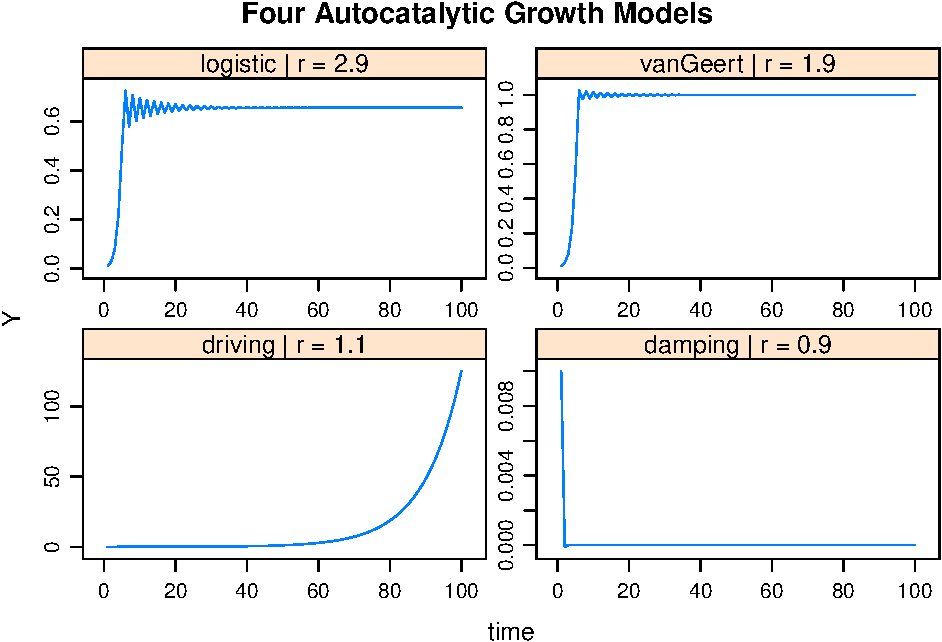
\includegraphics{DCS1617_files/figure-latex/unnamed-chunk-28-1.pdf}

\subsubsection*{The return plot}\label{the-return-plot-1}
\addcontentsline{toc}{subsubsection}{The return plot}

To create a return plot the values of \(Y\) have to be shifted by a
certain lag. The functions \texttt{lead()} and \texttt{lag()} in
\texttt{package::dplyr} are excellent for this purpose (note that
\texttt{dplyr::lag()} behaves different from \texttt{stats::lag()}).

\begin{Shaded}
\begin{Highlighting}[]
\CommentTok{# Function lag() and lead()}
\KeywordTok{require}\NormalTok{(dplyr)}

\CommentTok{# Get exponential growth}
\NormalTok{Y1 <-}\StringTok{ }\KeywordTok{growth.ac}\NormalTok{(}\DataTypeTok{Y0 =} \NormalTok{.}\DecValTok{9}\NormalTok{, }\DataTypeTok{r =} \NormalTok{.}\DecValTok{9}\NormalTok{, }\DataTypeTok{N =} \DecValTok{1000}\NormalTok{, }\DataTypeTok{type =} \StringTok{"driving"}\NormalTok{)}
\CommentTok{# Get logistic growth in the chaotic regime}
\NormalTok{Y2 <-}\StringTok{ }\KeywordTok{growth.ac}\NormalTok{(}\DataTypeTok{r =} \DecValTok{4}\NormalTok{, }\DataTypeTok{N =} \DecValTok{1000}\NormalTok{, }\DataTypeTok{type =} \StringTok{"logistic"}\NormalTok{)}
\CommentTok{# Use the `lag` function from package `dplyr`}
\NormalTok{op <-}\StringTok{ }\KeywordTok{par}\NormalTok{(}\DataTypeTok{mfrow =} \KeywordTok{c}\NormalTok{(}\DecValTok{1}\NormalTok{,}\DecValTok{2}\NormalTok{), }\DataTypeTok{pty =} \StringTok{"s"}\NormalTok{)}
\KeywordTok{plot}\NormalTok{(}\KeywordTok{lag}\NormalTok{(Y1), Y1, }\DataTypeTok{xy.labels =} \OtherTok{FALSE}\NormalTok{, }\DataTypeTok{pch =} \StringTok{"."}\NormalTok{, }\DataTypeTok{xlim =} \KeywordTok{c}\NormalTok{(}\DecValTok{0}\NormalTok{,}\DecValTok{1}\NormalTok{), }\DataTypeTok{ylim =} \KeywordTok{c}\NormalTok{(}\DecValTok{0}\NormalTok{,}\DecValTok{1}\NormalTok{), }\DataTypeTok{xlab =} \StringTok{"Y(t)"}\NormalTok{, }\DataTypeTok{ylab =} \StringTok{"Y(t+1)"}\NormalTok{,}
     \DataTypeTok{main =} \KeywordTok{expression}\NormalTok{(}\KeywordTok{paste}\NormalTok{(Y[t}\DecValTok{+1}\NormalTok{]==r*Y[t])))}
\KeywordTok{plot}\NormalTok{(}\KeywordTok{lag}\NormalTok{(Y2), Y2, }\DataTypeTok{xy.labels =} \OtherTok{FALSE}\NormalTok{, }\DataTypeTok{pch =} \StringTok{"."}\NormalTok{, }\DataTypeTok{xlim =} \KeywordTok{c}\NormalTok{(}\DecValTok{0}\NormalTok{,}\DecValTok{1}\NormalTok{), }\DataTypeTok{ylim =} \KeywordTok{c}\NormalTok{(}\DecValTok{0}\NormalTok{,}\DecValTok{1}\NormalTok{), }\DataTypeTok{xlab =} \StringTok{"Y(t)"}\NormalTok{, }\DataTypeTok{ylab =} \StringTok{"Y(t+1)"}\NormalTok{,}
     \DataTypeTok{main =} \KeywordTok{expression}\NormalTok{(}\KeywordTok{paste}\NormalTok{(Y[t}\DecValTok{+1}\NormalTok{]==r*Y[t]*(}\DecValTok{1}\NormalTok{-Y[t]))))}
\end{Highlighting}
\end{Shaded}

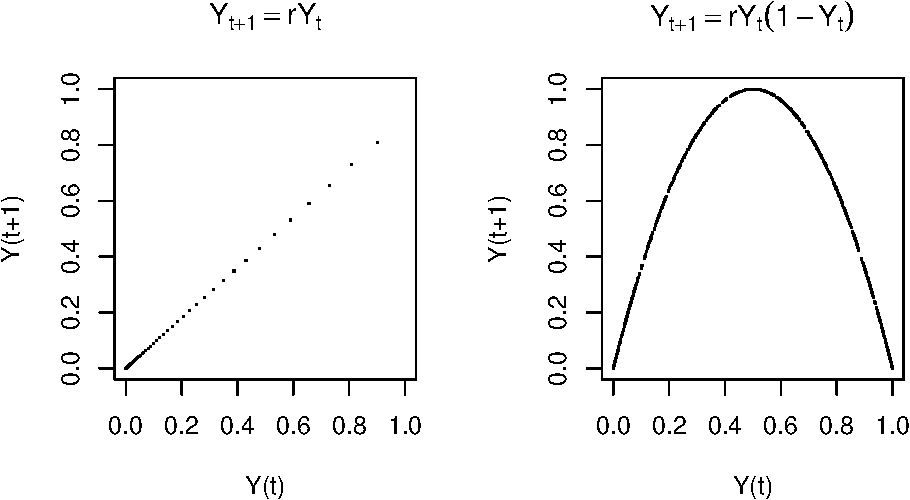
\includegraphics{DCS1617_files/figure-latex/unnamed-chunk-29-1.pdf}

\begin{Shaded}
\begin{Highlighting}[]
\KeywordTok{par}\NormalTok{(op)}
\end{Highlighting}
\end{Shaded}

Use \texttt{l\_ply()} from \texttt{package::plyr} to create return plots
with different lags. The \textbf{l\_} before \textbf{ply} means the
function will take a \textbf{l}ist as input to a function, but it will
not expect any data to be returned, for example in the case of a
function that is used to plot something.

\begin{Shaded}
\begin{Highlighting}[]
\CommentTok{# Explore different lags}
\NormalTok{op <-}\StringTok{ }\KeywordTok{par}\NormalTok{(}\DataTypeTok{mfrow =} \KeywordTok{c}\NormalTok{(}\DecValTok{1}\NormalTok{,}\DecValTok{2}\NormalTok{), }\DataTypeTok{pty =} \StringTok{"s"}\NormalTok{)}
\KeywordTok{l_ply}\NormalTok{(}\DecValTok{1}\NormalTok{:}\DecValTok{4}\NormalTok{, function(l) }\KeywordTok{plot}\NormalTok{(}\KeywordTok{lag}\NormalTok{(Y2, }\DataTypeTok{n =} \NormalTok{l), Y2, }\DataTypeTok{xy.labels =} \OtherTok{FALSE}\NormalTok{, }\DataTypeTok{pch =} \StringTok{"."}\NormalTok{, }\DataTypeTok{xlim =} \KeywordTok{c}\NormalTok{(}\DecValTok{0}\NormalTok{,}\DecValTok{1}\NormalTok{), }\DataTypeTok{ylim =} \KeywordTok{c}\NormalTok{(}\DecValTok{0}\NormalTok{,}\DecValTok{1}\NormalTok{), }\DataTypeTok{xlab =} \StringTok{"Y(t)"}\NormalTok{, }\DataTypeTok{ylab =} \KeywordTok{paste0}\NormalTok{(}\StringTok{"Y(t+"}\NormalTok{,l,}\StringTok{")"}\NormalTok{), }\DataTypeTok{cex =} \NormalTok{.}\DecValTok{8}\NormalTok{))}
\end{Highlighting}
\end{Shaded}

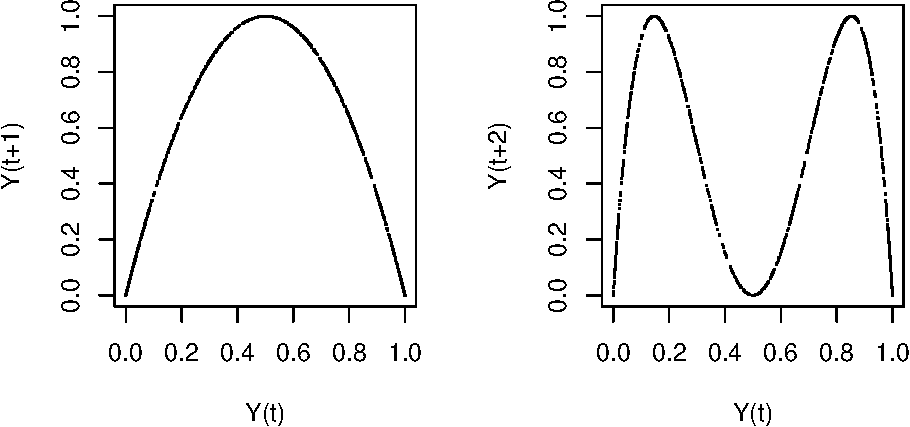
\includegraphics{DCS1617_files/figure-latex/unnamed-chunk-30-1.pdf}
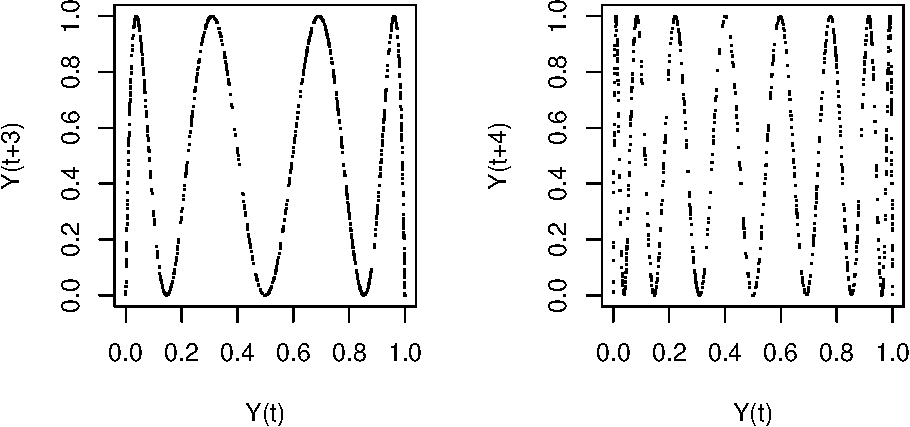
\includegraphics{DCS1617_files/figure-latex/unnamed-chunk-30-2.pdf}

\begin{Shaded}
\begin{Highlighting}[]
\KeywordTok{par}\NormalTok{(op)}
\end{Highlighting}
\end{Shaded}

\subsection{\texorpdfstring{Solutions in
\texttt{Matlab}}{Solutions in Matlab}}\label{solutions-in-matlab}

For \texttt{Matlab} we provide an example of a simple
\texttt{for\ ...\ next} loop, which should be easy to translate to
\texttt{R} if you want to.

\subsubsection*{Linear Map}\label{linear-map}
\addcontentsline{toc}{subsubsection}{Linear Map}

\begin{Shaded}
\begin{Highlighting}[]
\NormalTok{%%%%%%%%%%%%%%}\StringTok{ }\NormalTok{COMPUTING TRAJECTORIES OF THE LOGISTIC MAP %%%%%}

\NormalTok\StringTok{ }\NormalTok{Set these parameters to manipulate the logistic map}

\NormalTok{r  =}\StringTok{ }\DecValTok{1}\NormalTok{,}\DecValTok{1}\NormalTok{;       % Control parameter value}

\NormalTok{Y0 =}\StringTok{ }\FloatTok{0.01}\NormalTok{;   % Initial condition}

\NormalTok{N  =}\StringTok{ }\DecValTok{100}\NormalTok{;     % Number of iterations}

\NormalTok
\NormalTok{Y =}\StringTok{ }\NormalTok{[Y0; }\OtherTok{NaN}\NormalTok{(}\KeywordTok{length}\NormalTok{(}\DecValTok{1}\NormalTok{:(N}\DecValTok{-1}\NormalTok{)),}\DecValTok{1}\NormalTok{)];   % This creates a vector Y of length N}

\NormalTok{% iterate values}
\NormalTok{for t =}\StringTok{ }\DecValTok{1}\NormalTok{:(N}\DecValTok{-1}\NormalTok{)}
 \KeywordTok{Y}\NormalTok{(t}\DecValTok{+1}\NormalTok{) =}\StringTok{ }\NormalTok{r*}\KeywordTok{Y}\NormalTok{(t);  }
\NormalTok{end}

\NormalTok\StringTok{ }\NormalTok{Graphs}

\KeywordTok{subplot}\NormalTok{(}\DecValTok{2}\NormalTok{,}\DecValTok{1}\NormalTok{,}\DecValTok{1}\NormalTok{)}
\NormalTok{% Create a graph the time series}
\KeywordTok{figure}\NormalTok{(}\DecValTok{1}\NormalTok{);}
\KeywordTok{set}\NormalTok{(gcf,}\StringTok{'Color'}\NormalTok{,}\StringTok{'white'}\NormalTok{);}
\KeywordTok{plot}\NormalTok{(Y,}\StringTok{'k'}\NormalTok{);}
\KeywordTok{xlabel}\NormalTok{(}\StringTok{'Time (discrete)'}\NormalTok{)}
\KeywordTok{ylabel}\NormalTok{(}\StringTok{'Time Evolution of Y'}\NormalTok{)}
\KeywordTok{title}\NormalTok{([\{}\StringTok{'Linear Map'}\NormalTok{\},\{[}\StringTok{'Y_0 = '} \KeywordTok{num2str}\NormalTok{(Y0) }\StringTok{', r = '} \KeywordTok{num2str}\NormalTok{(r)]\}])}

\KeywordTok{subplot}\NormalTok{(}\DecValTok{2}\NormalTok{,}\DecValTok{1}\NormalTok{,}\DecValTok{2}\NormalTok{)}
\NormalTok{% Create a graph the return plot}
\KeywordTok{set}\NormalTok{(gcf,}\StringTok{'Color'}\NormalTok{,}\StringTok{'white'}\NormalTok{);}
\KeywordTok{plot}\NormalTok{(}\KeywordTok{Y}\NormalTok{(}\DecValTok{1}\NormalTok{:}\KeywordTok{length}\NormalTok{(Y)-}\DecValTok{1}\NormalTok{),}\KeywordTok{Y}\NormalTok{(}\DecValTok{2}\NormalTok{:}\KeywordTok{length}\NormalTok{(Y)),}\StringTok{'.k'}\NormalTok{);}
\KeywordTok{xlabel}\NormalTok{(}\StringTok{'Y(t)'}\NormalTok{)}
\KeywordTok{ylabel}\NormalTok{(}\StringTok{'Y(t+1)'}\NormalTok{)}
\KeywordTok{title}\NormalTok{([\{}\StringTok{'Return Plot'}\NormalTok{\},\{[}\StringTok{'Y_0 = '} \KeywordTok{num2str}\NormalTok{(Y0) }\StringTok{', r = '} \KeywordTok{num2str}\NormalTok{(r)]\}])}
\NormalTok{axis square}
\end{Highlighting}
\end{Shaded}

\subsubsection*{Logistic Map}\label{logistic-map}
\addcontentsline{toc}{subsubsection}{Logistic Map}

\begin{Shaded}
\begin{Highlighting}[]
\NormalTok{%%%%%%%%%%%%%%}\StringTok{ }\NormalTok{COMPUTING TRAJECTORIES OF THE LOGISTIC MAP %%%%%}

\NormalTok\StringTok{ }\NormalTok{Set these parameters to manipulate the logistic map}

\NormalTok{r  =}\StringTok{ }\DecValTok{4}\NormalTok{;       % Control parameter value}

\NormalTok{Y0 =}\StringTok{ }\FloatTok{0.08}\NormalTok{;   % Initial condition}

\NormalTok{N  =}\StringTok{ }\DecValTok{100}\NormalTok{;     % Number of iterations}

\NormalTok
\NormalTok{Y =}\StringTok{ }\NormalTok{[Y0; }\OtherTok{NaN}\NormalTok{(}\KeywordTok{length}\NormalTok{(}\DecValTok{1}\NormalTok{:(N}\DecValTok{-1}\NormalTok{)),}\DecValTok{1}\NormalTok{)];   % This creates a vector Y of length N}

\NormalTok{% iterate values}
\NormalTok{for t =}\StringTok{ }\DecValTok{1}\NormalTok{:(N}\DecValTok{-1}\NormalTok{)}
 \KeywordTok{Y}\NormalTok{(t}\DecValTok{+1}\NormalTok{) =}\StringTok{ }\NormalTok{r*}\KeywordTok{Y}\NormalTok{(t)*(}\DecValTok{1}\NormalTok{-}\KeywordTok{Y}\NormalTok{(t));  }
\NormalTok{end}

\NormalTok\StringTok{ }\NormalTok{Graphs}

\KeywordTok{subplot}\NormalTok{(}\DecValTok{2}\NormalTok{,}\DecValTok{1}\NormalTok{,}\DecValTok{1}\NormalTok{)}
\NormalTok{% Create a graph the time series}
\KeywordTok{figure}\NormalTok{(}\DecValTok{1}\NormalTok{);}
\KeywordTok{set}\NormalTok{(gcf,}\StringTok{'Color'}\NormalTok{,}\StringTok{'white'}\NormalTok{);}
\KeywordTok{plot}\NormalTok{(Y,}\StringTok{'k'}\NormalTok{);}
\KeywordTok{xlabel}\NormalTok{(}\StringTok{'Time (discrete)'}\NormalTok{)}
\KeywordTok{ylabel}\NormalTok{(}\StringTok{'Time Evolution of Y'}\NormalTok{)}
\KeywordTok{title}\NormalTok{([\{}\StringTok{'Logisitc Map'}\NormalTok{\},\{[}\StringTok{'Y_0 = '} \KeywordTok{num2str}\NormalTok{(Y0) }\StringTok{', r = '} \KeywordTok{num2str}\NormalTok{(r)]\}])}

\KeywordTok{subplot}\NormalTok{(}\DecValTok{2}\NormalTok{,}\DecValTok{1}\NormalTok{,}\DecValTok{2}\NormalTok{)}
\NormalTok{% Create a graph the return plot}
\KeywordTok{set}\NormalTok{(gcf,}\StringTok{'Color'}\NormalTok{,}\StringTok{'white'}\NormalTok{);}
\KeywordTok{plot}\NormalTok{(}\KeywordTok{Y}\NormalTok{(}\DecValTok{1}\NormalTok{:}\KeywordTok{length}\NormalTok{(Y)-}\DecValTok{1}\NormalTok{),}\KeywordTok{Y}\NormalTok{(}\DecValTok{2}\NormalTok{:}\KeywordTok{length}\NormalTok{(Y)),}\StringTok{'.k'}\NormalTok{);}
\KeywordTok{xlabel}\NormalTok{(}\StringTok{'Y(t)'}\NormalTok{)}
\KeywordTok{ylabel}\NormalTok{(}\StringTok{'Y(t+1)'}\NormalTok{)}
\KeywordTok{title}\NormalTok{([\{}\StringTok{'Return Plot'}\NormalTok{\},\{[}\StringTok{'Y_0 = '} \KeywordTok{num2str}\NormalTok{(Y0) }\StringTok{', r = '} \KeywordTok{num2str}\NormalTok{(r)]\}])}
\NormalTok{axis square}
\end{Highlighting}
\end{Shaded}

\begin{figure}[htbp]
\centering
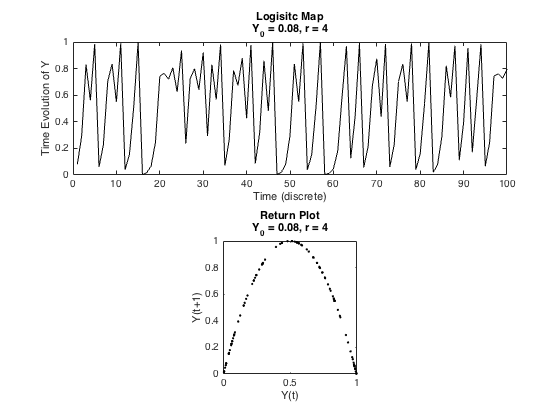
\includegraphics{images/logisticmap_Matlab.png}
\caption{Solution Logistic Map - Matlab}
\end{figure}

\begin{center}\rule{0.5\linewidth}{\linethickness}\end{center}

\chapter{\texorpdfstring{\textbf{Mathematics of Change
II}}{Mathematics of Change II}}\label{mathematics-of-change-ii}

Solutions to assignments in section \ref{moc2ass}

\begin{itemize}
\tightlist
\item
  Time-varying parameters
\item
  Predator-prey dynamics
\end{itemize}

\section{Time-varying parameters}\label{time-varying-parameters}

\subsection*{Solutions in a
spreadsheet}\label{solutions-in-a-spreadsheet-1}
\addcontentsline{toc}{subsection}{Solutions in a spreadsheet}

\begin{itemize}
\tightlist
\item
  \href{https://docs.google.com/spreadsheets/d/1DAg0u-zMFOIvRSDOZDxqnzyS0HQJg4FIXzJIMvEMwiI/edit?usp=sharing}{Van
  Geert, including jumps and stages}.
\end{itemize}

\subsection{\texorpdfstring{Solutions in
\texttt{R}}{Solutions in R}}\label{solutions-in-r-1}

\subsubsection*{The growth model by Van Geert
(1991)}\label{the-growth-model-by-van-geert-1991-1}
\addcontentsline{toc}{subsubsection}{The growth model by Van Geert
(1991)}

Different values for \texttt{r}:

\begin{Shaded}
\begin{Highlighting}[]
\KeywordTok{library}\NormalTok{(plyr)}
\CommentTok{# Parameters}
\NormalTok{rs <-}\StringTok{ }\KeywordTok{c}\NormalTok{(}\FloatTok{1.2}\NormalTok{, }\FloatTok{2.2}\NormalTok{, }\FloatTok{2.5}\NormalTok{, }\FloatTok{2.7}\NormalTok{, }\FloatTok{2.9}\NormalTok{, }\DecValTok{3}\NormalTok{)}
\CommentTok{# Plot }
\NormalTok{op <-}\StringTok{ }\KeywordTok{par}\NormalTok{(}\DataTypeTok{mfrow=}\KeywordTok{c}\NormalTok{(}\DecValTok{1}\NormalTok{,}\DecValTok{2}\NormalTok{))}
\KeywordTok{l_ply}\NormalTok{(rs,function(r)\{}\KeywordTok{plot}\NormalTok{(}\KeywordTok{growth.ac}\NormalTok{(}\DataTypeTok{r =} \NormalTok{r,  }\DataTypeTok{Y0 =} \FloatTok{0.01}\NormalTok{, }\DataTypeTok{type =} \StringTok{"vanGeert"}\NormalTok{),}
                          \DataTypeTok{ylim =} \KeywordTok{c}\NormalTok{(}\DecValTok{0}\NormalTok{,}\FloatTok{1.4}\NormalTok{), }\DataTypeTok{ylab =} \StringTok{"L(t)"}\NormalTok{, }\DataTypeTok{main =} \KeywordTok{paste}\NormalTok{(}\StringTok{"r ="}\NormalTok{,r))\})}
\end{Highlighting}
\end{Shaded}

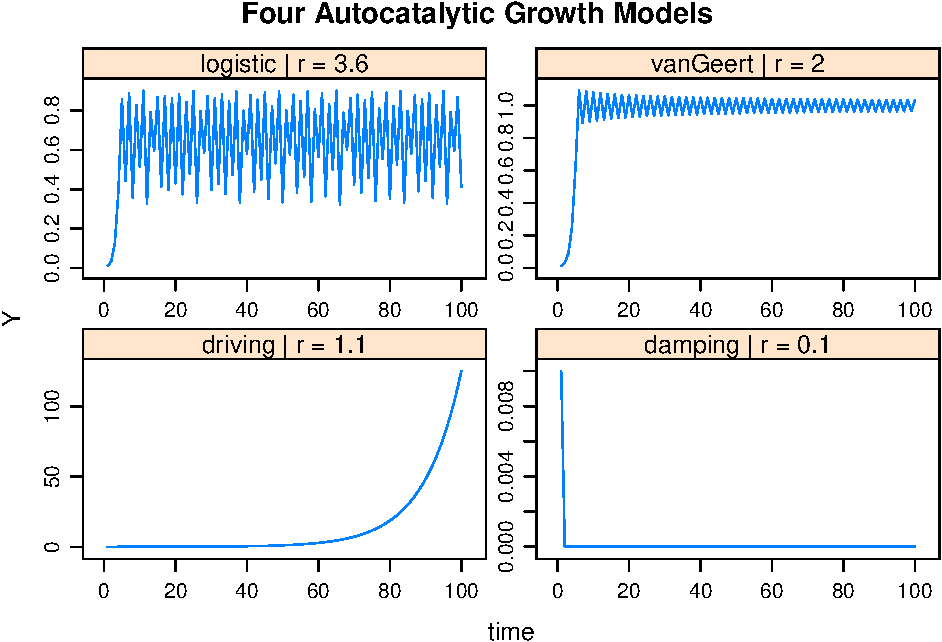
\includegraphics{DCS1617_files/figure-latex/unnamed-chunk-33-1.pdf}
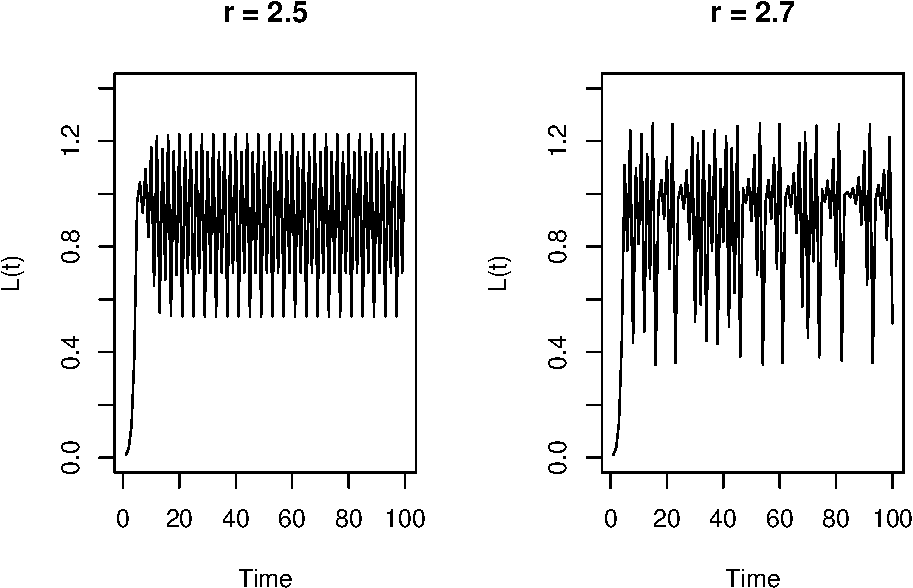
\includegraphics{DCS1617_files/figure-latex/unnamed-chunk-33-2.pdf}
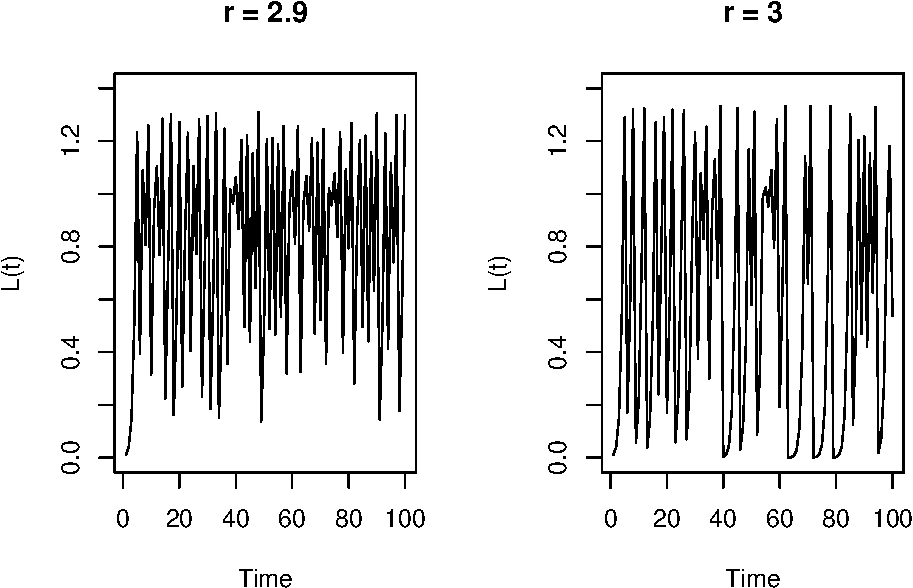
\includegraphics{DCS1617_files/figure-latex/unnamed-chunk-33-3.pdf}

\begin{Shaded}
\begin{Highlighting}[]
\KeywordTok{par}\NormalTok{(op)}
\end{Highlighting}
\end{Shaded}

Different values for \(k\) reveal that the dispersion of values
(variance) increases if the carrying capacity increases. This occurs
because we are dealing with nonlinear changes to the values of \(Y\) and
if larger values of \(Y\) are allowed by a hihger \(k\), these values
will be amplified once they occur.

\begin{Shaded}
\begin{Highlighting}[]
\CommentTok{# Parameters}
\NormalTok{ks <-}\StringTok{ }\KeywordTok{c}\NormalTok{(}\FloatTok{0.5}\NormalTok{, }\FloatTok{0.75}\NormalTok{, }\DecValTok{1}\NormalTok{, }\FloatTok{1.5}\NormalTok{)}
\CommentTok{# Plot }
\NormalTok{op <-}\StringTok{ }\KeywordTok{par}\NormalTok{(}\DataTypeTok{mfrow=}\KeywordTok{c}\NormalTok{(}\DecValTok{1}\NormalTok{,}\DecValTok{2}\NormalTok{))}
\KeywordTok{l_ply}\NormalTok{(ks,function(k)\{}\KeywordTok{plot}\NormalTok{(}\KeywordTok{growth.ac}\NormalTok{(}\DataTypeTok{r =} \FloatTok{2.9}\NormalTok{, }\DataTypeTok{k =} \NormalTok{k, }\DataTypeTok{Y0 =} \FloatTok{0.01}\NormalTok{, }\DataTypeTok{type =} \StringTok{"vanGeert"}\NormalTok{),}
                          \DataTypeTok{ylim =} \KeywordTok{c}\NormalTok{(}\DecValTok{0}\NormalTok{, }\DecValTok{2}\NormalTok{), }\DataTypeTok{ylab =} \StringTok{"L(t)"}\NormalTok{, }\DataTypeTok{main =} \KeywordTok{paste}\NormalTok{(}\StringTok{"k ="}\NormalTok{,k))\})}
\end{Highlighting}
\end{Shaded}

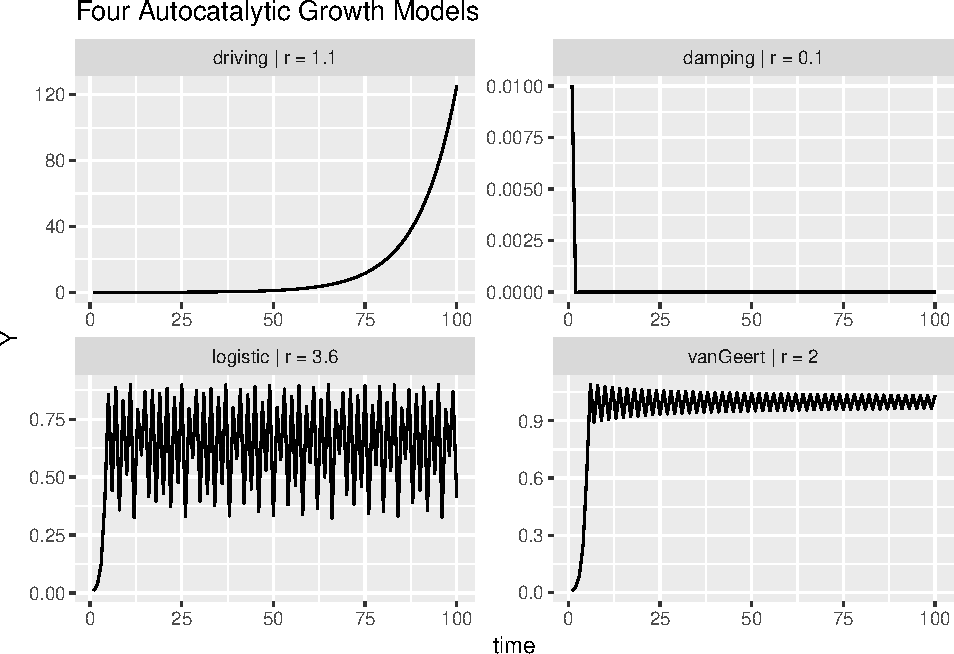
\includegraphics{DCS1617_files/figure-latex/unnamed-chunk-34-1.pdf}
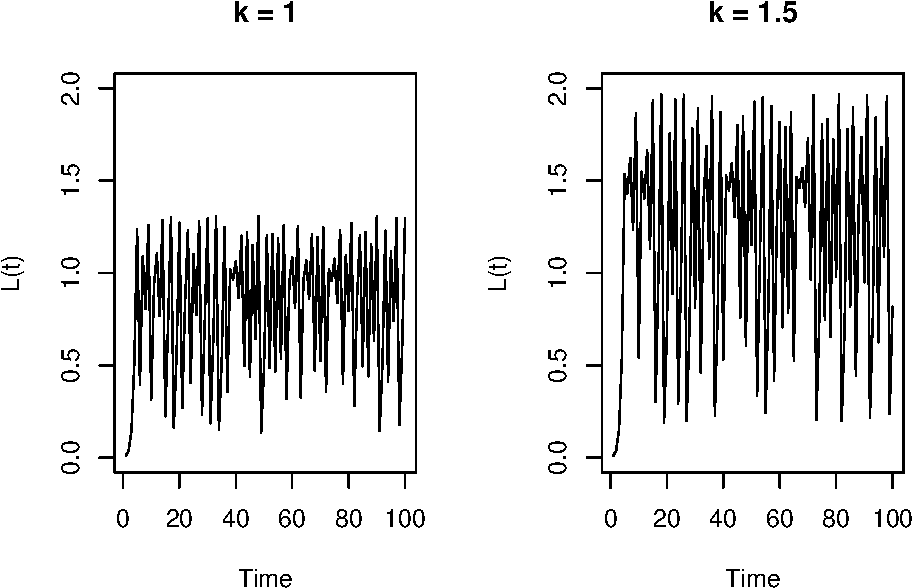
\includegraphics{DCS1617_files/figure-latex/unnamed-chunk-34-2.pdf}

\begin{Shaded}
\begin{Highlighting}[]
\KeywordTok{par}\NormalTok{(op)}
\end{Highlighting}
\end{Shaded}

\subsubsection*{Stages and Jumps}\label{stages-and-jumps}
\addcontentsline{toc}{subsubsection}{Stages and Jumps}

\begin{Shaded}
\begin{Highlighting}[]
\NormalTok{growth.ac.cond <-}\StringTok{ }\NormalTok{function(}\DataTypeTok{Y0 =} \FloatTok{0.01}\NormalTok{, }\DataTypeTok{r =} \FloatTok{0.1}\NormalTok{, }\DataTypeTok{k =} \DecValTok{2}\NormalTok{, }\DataTypeTok{cond =} \KeywordTok{cbind.data.frame}\NormalTok{(}\DataTypeTok{Y =} \FloatTok{0.2}\NormalTok{, }\DataTypeTok{par =} \StringTok{"r"}\NormalTok{, }\DataTypeTok{val =} \DecValTok{2}\NormalTok{), }\DataTypeTok{N =} \DecValTok{100}\NormalTok{)\{}
    \CommentTok{# Create a vector Y of length N, which has value Y0 at Y[1]}
    \NormalTok{Y <-}\StringTok{ }\KeywordTok{c}\NormalTok{(Y0, }\KeywordTok{rep}\NormalTok{(}\OtherTok{NA}\NormalTok{, N}\DecValTok{-1}\NormalTok{))}
    \CommentTok{# Iterate N steps of the difference equation with values passed for Y0, k and r.}
    \NormalTok{cnt <-}\StringTok{ }\DecValTok{1}
    \NormalTok{for(t in }\KeywordTok{seq_along}\NormalTok{(Y))\{}
        \CommentTok{# Check if the current value of Y is greater than the threshold for the current conditional rule in cond}
        \NormalTok{if(Y[t] >}\StringTok{ }\NormalTok{cond$Y[cnt])\{}
            \CommentTok{# If the threshold is surpassed, change the parameter settings by evaluating: cond$par = cond$val }
            \KeywordTok{eval}\NormalTok{(}\KeywordTok{parse}\NormalTok{(}\DataTypeTok{text =} \KeywordTok{paste}\NormalTok{(cond$par[cnt], }\StringTok{"="}\NormalTok{, cond$val[cnt])))}
            \CommentTok{# Update the counter if there is another conditional rule in cond}
            \NormalTok{if(cnt <}\StringTok{ }\KeywordTok{nrow}\NormalTok{(cond))\{cnt <-}\StringTok{ }\NormalTok{cnt +}\StringTok{ }\DecValTok{1}\NormalTok{\}}
        \NormalTok{\}}
        \CommentTok{# Van Geert growth model}
        \NormalTok{Y[[t}\DecValTok{+1}\NormalTok{]] <-}\StringTok{ }\NormalTok{Y[t] *}\StringTok{ }\NormalTok{(}\DecValTok{1} \NormalTok{+}\StringTok{ }\NormalTok{r -}\StringTok{ }\NormalTok{r *}\StringTok{ }\NormalTok{Y[t] /}\StringTok{ }\NormalTok{k)}
    \NormalTok{\}}
    \KeywordTok{return}\NormalTok{(}\KeywordTok{ts}\NormalTok{(Y))}
\NormalTok{\}}

\CommentTok{# Plot with the default settings (same as first step in the assignment) }
\KeywordTok{xyplot}\NormalTok{(}\KeywordTok{growth.ac.cond}\NormalTok{())}
\end{Highlighting}
\end{Shaded}

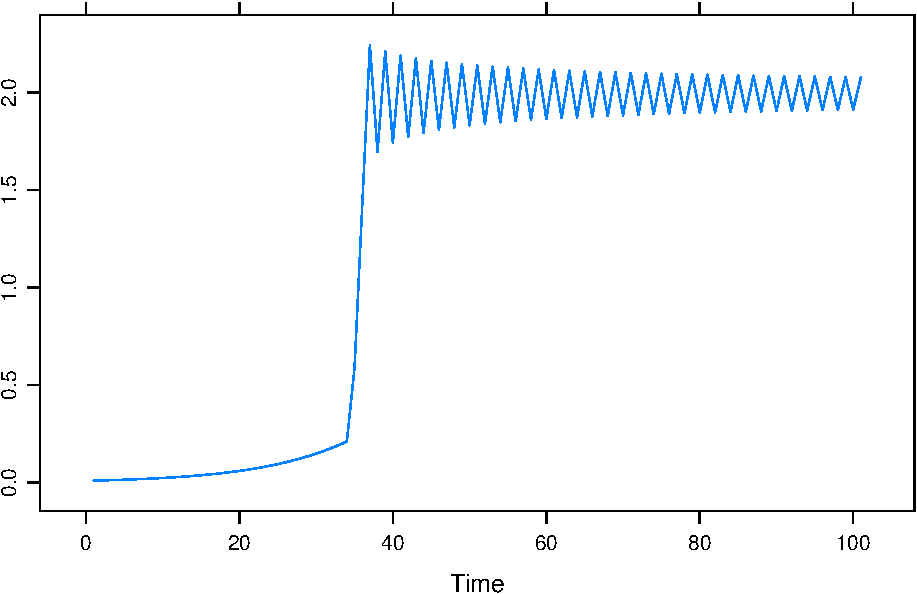
\includegraphics{DCS1617_files/figure-latex/unnamed-chunk-35-1.pdf}

The `trick' used here is to define the function such that it can take a
set of conditional rules and apply them sequentially during the
iterations. The conditiona rule is passed as a \texttt{data.frame}, but
one could also use a \texttt{list} object.

\begin{Shaded}
\begin{Highlighting}[]
\NormalTok{(cond <-}\StringTok{ }\KeywordTok{cbind.data.frame}\NormalTok{(}\DataTypeTok{Y =} \KeywordTok{c}\NormalTok{(}\FloatTok{0.2}\NormalTok{, }\FloatTok{0.6}\NormalTok{), }\DataTypeTok{par =} \KeywordTok{c}\NormalTok{(}\StringTok{"r"}\NormalTok{, }\StringTok{"r"}\NormalTok{), }\DataTypeTok{val =} \KeywordTok{c}\NormalTok{(}\FloatTok{0.5}\NormalTok{, }\FloatTok{0.1}\NormalTok{)))}
\end{Highlighting}
\end{Shaded}

\begin{verbatim}
    Y par val
1 0.2   r 0.5
2 0.6   r 0.1
\end{verbatim}

\begin{Shaded}
\begin{Highlighting}[]
\KeywordTok{xyplot}\NormalTok{(}\KeywordTok{growth.ac.cond}\NormalTok{(}\DataTypeTok{cond=}\NormalTok{cond))}
\end{Highlighting}
\end{Shaded}

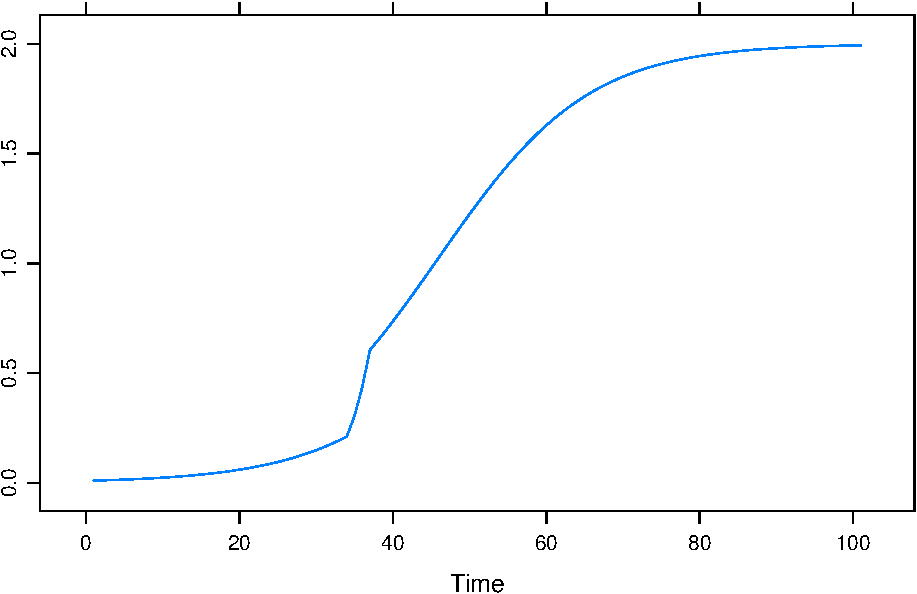
\includegraphics{DCS1617_files/figure-latex/unnamed-chunk-36-1.pdf}

Or, combine a change of \texttt{r} and a change of \texttt{k}

\begin{Shaded}
\begin{Highlighting}[]
\NormalTok{(cond <-}\StringTok{ }\KeywordTok{cbind.data.frame}\NormalTok{(}\DataTypeTok{Y =} \KeywordTok{c}\NormalTok{(}\FloatTok{0.2}\NormalTok{, }\FloatTok{1.99}\NormalTok{), }\DataTypeTok{par =} \KeywordTok{c}\NormalTok{(}\StringTok{"r"}\NormalTok{, }\StringTok{"k"}\NormalTok{), }\DataTypeTok{val =} \KeywordTok{c}\NormalTok{(}\FloatTok{0.5}\NormalTok{, }\DecValTok{3}\NormalTok{)))}
\end{Highlighting}
\end{Shaded}

\begin{verbatim}
     Y par val
1 0.20   r 0.5
2 1.99   k 3.0
\end{verbatim}

\begin{Shaded}
\begin{Highlighting}[]
\KeywordTok{xyplot}\NormalTok{(}\KeywordTok{growth.ac.cond}\NormalTok{(}\DataTypeTok{cond=}\NormalTok{cond))}
\end{Highlighting}
\end{Shaded}

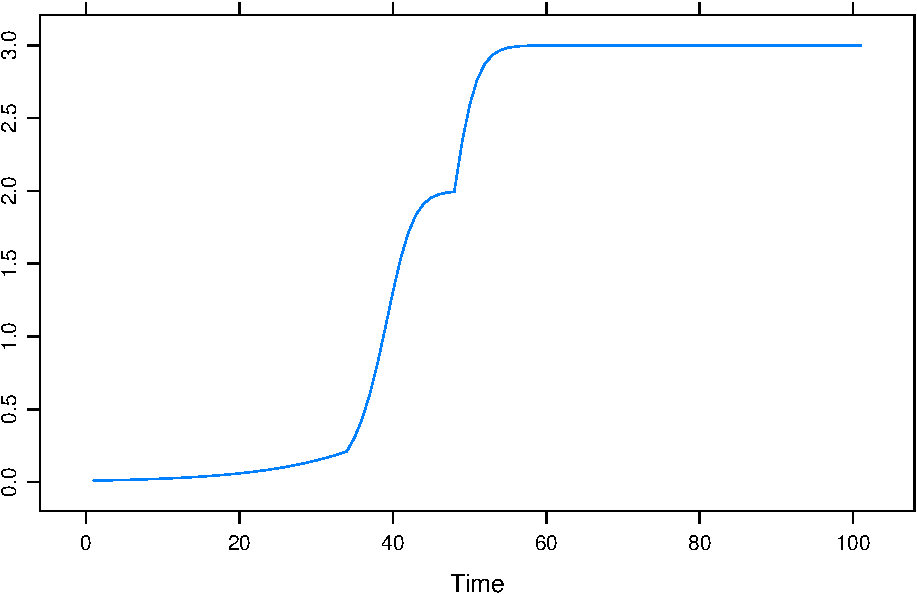
\includegraphics{DCS1617_files/figure-latex/unnamed-chunk-37-1.pdf}

\begin{Shaded}
\begin{Highlighting}[]
\CommentTok{# A fantasy growth process}
\NormalTok{(cond <-}\StringTok{ }\KeywordTok{cbind.data.frame}\NormalTok{(}\DataTypeTok{Y =} \KeywordTok{c}\NormalTok{(}\FloatTok{0.1}\NormalTok{, }\FloatTok{1.99}\NormalTok{, }\FloatTok{1.999}\NormalTok{, }\FloatTok{2.5}\NormalTok{, }\FloatTok{2.9}\NormalTok{), }\DataTypeTok{par =} \KeywordTok{c}\NormalTok{(}\StringTok{"r"}\NormalTok{, }\StringTok{"k"}\NormalTok{, }\StringTok{"r"}\NormalTok{, }\StringTok{"r"}\NormalTok{,}\StringTok{"k"}\NormalTok{), }\DataTypeTok{val =} \KeywordTok{c}\NormalTok{(}\FloatTok{0.3}\NormalTok{, }\DecValTok{3}\NormalTok{, }\FloatTok{0.9}\NormalTok{, }\FloatTok{0.1}\NormalTok{, }\FloatTok{1.3}\NormalTok{)))}
\end{Highlighting}
\end{Shaded}

\begin{verbatim}
      Y par val
1 0.100   r 0.3
2 1.990   k 3.0
3 1.999   r 0.9
4 2.500   r 0.1
5 2.900   k 1.3
\end{verbatim}

\begin{Shaded}
\begin{Highlighting}[]
\KeywordTok{xyplot}\NormalTok{(}\KeywordTok{growth.ac.cond}\NormalTok{(}\DataTypeTok{cond=}\NormalTok{cond))}
\end{Highlighting}
\end{Shaded}

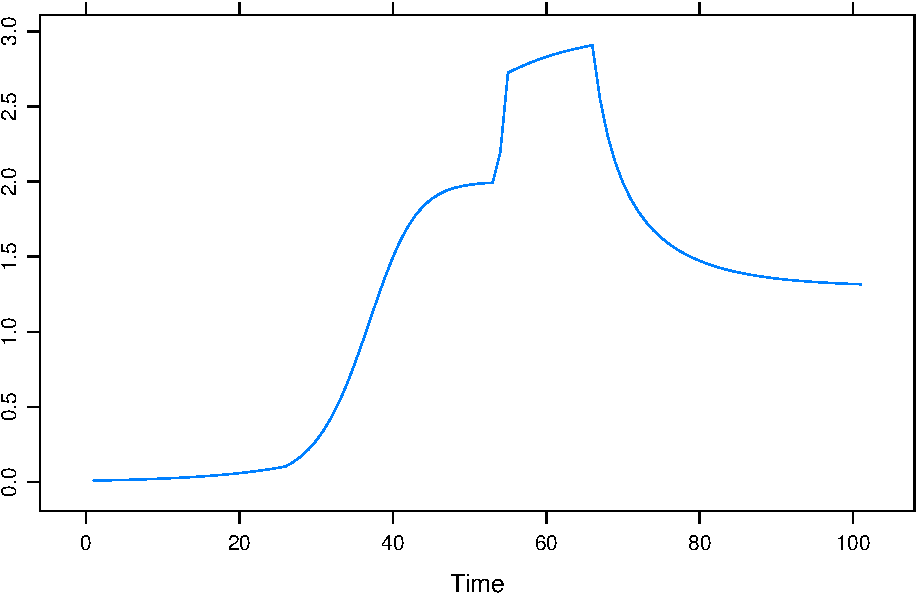
\includegraphics{DCS1617_files/figure-latex/unnamed-chunk-37-2.pdf}

\subsubsection*{Connected Growers}\label{connected-growers-1}
\addcontentsline{toc}{subsubsection}{Connected Growers}

Somewhat more realstic would be to model a change of \texttt{r} as
dependent on the values of another process. The proper `dynamical' way
to do this would be to define a coupled system of difference or
differential equations in which the interaction dynamics regulate
growth. An example is the predator-prey system discussed in the next
assignment.

Using the `conditional' rules on a number of seperate processes will
`work' as a model, but it isn't exactly what is meant by
\emph{interaction dynamics}, or \emph{multiplicative interactions}.
Basically, these processes will be independent and non-interacting. The
conditional rules that change the parameters are `given'.

\begin{Shaded}
\begin{Highlighting}[]
\CommentTok{# Generate 3 timeseries}
\NormalTok{Y1 <-}\StringTok{ }\KeywordTok{growth.ac}\NormalTok{(}\DataTypeTok{k =} \DecValTok{2}\NormalTok{, }\DataTypeTok{r =}\NormalTok{.}\DecValTok{2}\NormalTok{, }\DataTypeTok{type =} \StringTok{"vanGeert"}\NormalTok{)}
\CommentTok{# Y2 and Y3 start at r = 0.001}
\NormalTok{Y3 <-}\StringTok{ }\NormalTok{Y2 <-}\StringTok{ }\KeywordTok{growth.ac}\NormalTok{(}\DataTypeTok{k =} \DecValTok{2}\NormalTok{, }\DataTypeTok{r =} \FloatTok{0.001}\NormalTok{, }\DataTypeTok{type =} \StringTok{"vanGeert"}\NormalTok{)}

\CommentTok{# Y2 and Y3 start when k is approached}
\NormalTok{c1 <-}\StringTok{ }\FloatTok{1.6}
\NormalTok{c2 <-}\StringTok{ }\FloatTok{2.2}
\NormalTok{Y2[Y1 >}\StringTok{ }\NormalTok{c1] <-}\StringTok{ }\KeywordTok{growth.ac}\NormalTok{(}\DataTypeTok{r =} \NormalTok{.}\DecValTok{3}\NormalTok{, }\DataTypeTok{k =} \DecValTok{3}\NormalTok{, }\DataTypeTok{type =} \StringTok{"vanGeert"}\NormalTok{, }\DataTypeTok{N =} \KeywordTok{sum}\NormalTok{(Y1 >}\StringTok{ }\NormalTok{c1))}
\NormalTok{Y3[Y2 >}\StringTok{ }\NormalTok{c2] <-}\StringTok{ }\KeywordTok{growth.ac}\NormalTok{(}\DataTypeTok{r =} \NormalTok{.}\DecValTok{5}\NormalTok{, }\DataTypeTok{k =} \DecValTok{4}\NormalTok{, }\DataTypeTok{type =} \StringTok{"vanGeert"}\NormalTok{, }\DataTypeTok{N =} \KeywordTok{sum}\NormalTok{(Y2 >}\StringTok{ }\NormalTok{c2))}

\CommentTok{# Make a nice plot}
\KeywordTok{ts.plot}\NormalTok{(Y1, Y2, Y3,}
        \DataTypeTok{gpars =} \KeywordTok{list}\NormalTok{(}\DataTypeTok{xlab =} \StringTok{"time (a.u.)"}\NormalTok{,}
                     \DataTypeTok{ylab =} \KeywordTok{expression}\NormalTok{(}\KeywordTok{Y}\NormalTok{(t)),}
                     \DataTypeTok{main =} \KeywordTok{expression}\NormalTok{(}\KeywordTok{paste}\NormalTok{(}\StringTok{"'Connected' Growers "}\NormalTok{,Y[t}\DecValTok{+1}\NormalTok{]==Y[t]*(}\DecValTok{1} \NormalTok{+}\StringTok{ }\NormalTok{r -}\StringTok{ }\NormalTok{r*Y[t]))),}
                     \DataTypeTok{lwd =} \KeywordTok{rep}\NormalTok{(}\DecValTok{2}\NormalTok{,}\DecValTok{3}\NormalTok{),}
                     \DataTypeTok{lty =} \KeywordTok{c}\NormalTok{(}\DecValTok{1}\NormalTok{:}\DecValTok{3}\NormalTok{),}
                     \DataTypeTok{col =} \KeywordTok{c}\NormalTok{(}\StringTok{"darkred"}\NormalTok{,}\StringTok{"darkblue"}\NormalTok{,}\StringTok{"darkgreen"}\NormalTok{)}
                     \NormalTok{)}
        \NormalTok{)}
\KeywordTok{legend}\NormalTok{(}\DecValTok{1}\NormalTok{, }\FloatTok{3.8}\NormalTok{, }\KeywordTok{c}\NormalTok{(}\StringTok{"Y1(0):  r = .2"}\NormalTok{,}
                 \KeywordTok{paste0}\NormalTok{(}\StringTok{"Y2("}\NormalTok{,}\KeywordTok{which}\NormalTok{(Y1 >}\StringTok{ }\NormalTok{c1)[}\DecValTok{1}\NormalTok{],}\StringTok{"): r = .3"}\NormalTok{), }
                 \KeywordTok{paste0}\NormalTok{(}\StringTok{"Y3("}\NormalTok{,}\KeywordTok{which}\NormalTok{(Y2 >}\StringTok{ }\NormalTok{c2)[}\DecValTok{1}\NormalTok{],}\StringTok{"): r = .5"}\NormalTok{)),}
       \DataTypeTok{lwd =} \KeywordTok{rep}\NormalTok{(}\DecValTok{2}\NormalTok{,}\DecValTok{3}\NormalTok{), }\DataTypeTok{lty =} \KeywordTok{c}\NormalTok{(}\DecValTok{1}\NormalTok{:}\DecValTok{3}\NormalTok{), }\DataTypeTok{col =} \KeywordTok{c}\NormalTok{(}\StringTok{"darkred"}\NormalTok{,}\StringTok{"darkblue"}\NormalTok{,}\StringTok{"darkgreen"}\NormalTok{), }\DataTypeTok{merge =} \OtherTok{TRUE}\NormalTok{)}
\end{Highlighting}
\end{Shaded}

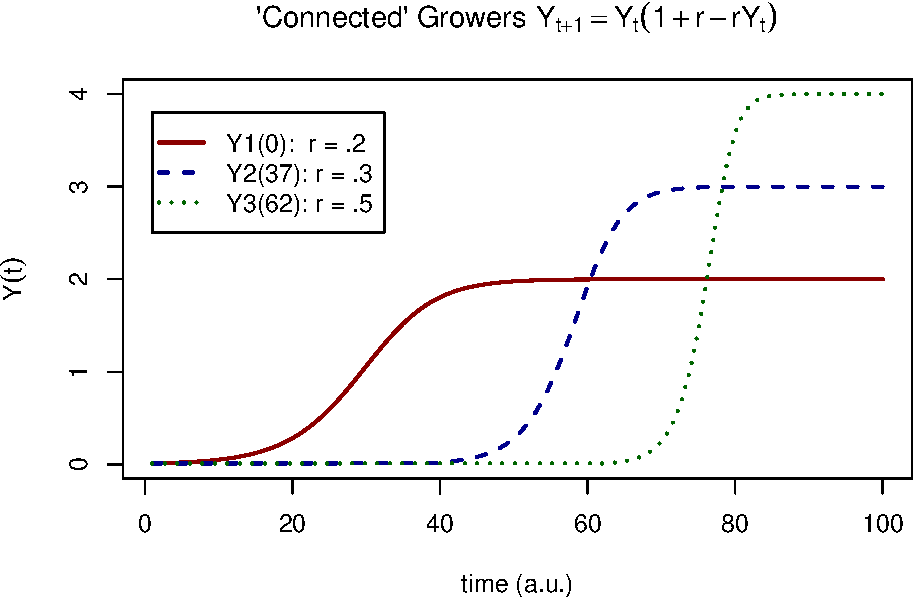
\includegraphics{DCS1617_files/figure-latex/unnamed-chunk-38-1.pdf}

\hypertarget{ppdsol}{\section{Predator-prey dynamics}\label{ppdsol}}

\href{\%7B\#moc1R\%7D}{\textbar{} jump to question \textbar{}}

\subsection*{Iterating 2D Maps and
Flows}\label{iterating-2d-maps-and-flows-1}
\addcontentsline{toc}{subsection}{Iterating 2D Maps and Flows}

In order to `solve' a differential equation for time using a method of
numerical integration, one could code it like in the spreadsheet
assignment. For \texttt{R} and \texttt{Matlab} there are so-called
\emph{solvers} available, functions that will do the integration for
you. Look at the
\href{http://www.inside-r.org/packages/cran/deSolve/docs/euler}{Examples
in package \texttt{deSolve}}.

\subsection*{Solutions in a
spreadsheet}\label{solutions-in-a-spreadsheet-2}
\addcontentsline{toc}{subsection}{Solutions in a spreadsheet}

\begin{itemize}
\tightlist
\item
  \href{https://docs.google.com/spreadsheets/d/1rZDEo8XYNCzhRWrWOli7DDB6f4m87p-hjYv2_KlBLa4/edit?usp=sharing}{Predator-Prey
  Dynamics}
\end{itemize}

\subsection{\texorpdfstring{Solutions in
\texttt{R}}{Solutions in R}}\label{solutions-in-r-2}

\subsubsection*{Euler's method and
more\ldots{}}\label{eulers-method-and-more-1}
\addcontentsline{toc}{subsubsection}{Euler's method and more\ldots{}}

The result of applying a method of numerical integration is called a
\textbf{numerical solution} of the differential equation. The
\textbf{analytical solution} is the equation which will give you a value
of \(Y\) for any point in time, given an initial value \(Y_0\). Systems
which have an analytical solution can be used to test the accuracy of
\textbf{numerical solutions}.

Remember that the analytical solution for the logistic equation is:

\begin{equation}
\frac{K}{1 + \left(\frac{K}{Y_0 - 1}\right) * e^{-r*t} }
\label{eq:logSol}
\end{equation}

We have the function \texttt{growth.ac()} and could easily adapt all the
functions to use Euler's method.\\
Below is a comparison of the analytic solution with Euler's method.

\begin{Shaded}
\begin{Highlighting}[]
\CommentTok{# Parameter settings}
\NormalTok{d <-}\StringTok{ }\DecValTok{1}
\NormalTok{N <-}\StringTok{ }\DecValTok{100}
\NormalTok{r <-}\StringTok{ }\NormalTok{.}\DecValTok{1}
\NormalTok{k <-}\StringTok{ }\DecValTok{1}
\NormalTok{Y0 <-}\StringTok{ }\FloatTok{0.01}

\NormalTok{Y <-}\StringTok{ }\KeywordTok{as.numeric}\NormalTok{(}\KeywordTok{c}\NormalTok{(Y0, }\KeywordTok{rep}\NormalTok{(}\OtherTok{NA}\NormalTok{,N}\DecValTok{-1}\NormalTok{)))}

\CommentTok{# Numerical integration of the logistic differential equation}
\NormalTok{Y.euler1 <-}\StringTok{ }\KeywordTok{ts}\NormalTok{( }\KeywordTok{sapply}\NormalTok{(}\KeywordTok{seq_along}\NormalTok{(Y), function(t) Y[[t}\DecValTok{+1}\NormalTok{]] <<-}\StringTok{ }\NormalTok{(r *}\StringTok{ }\NormalTok{Y[t] *}\StringTok{ }\NormalTok{(k -}\StringTok{ }\NormalTok{Y[t])) *}\StringTok{ }\NormalTok{d +}\StringTok{ }\NormalTok{Y[t] )) }
\NormalTok{Y.euler2 <-}\StringTok{ }\KeywordTok{ts}\NormalTok{( }\KeywordTok{sapply}\NormalTok{(}\KeywordTok{seq_along}\NormalTok{(Y), function(t) Y[[t}\DecValTok{+1}\NormalTok{]] <<-}\StringTok{ }\NormalTok{(r *}\StringTok{ }\NormalTok{Y[t] *}\StringTok{ }\NormalTok{(k -}\StringTok{ }\NormalTok{Y[t])) *}\StringTok{ }\NormalTok{(d}\FloatTok{+.1}\NormalTok{) +}\StringTok{ }\NormalTok{Y[t] )) }

\NormalTok{## analytical solution}
\NormalTok{Y.analytic <-}\StringTok{ }\KeywordTok{ts}\NormalTok{( k /}\StringTok{ }\NormalTok{(}\DecValTok{1} \NormalTok{+}\StringTok{ }\NormalTok{(k /}\StringTok{ }\NormalTok{Y0 -}\StringTok{ }\DecValTok{1}\NormalTok{) *}\StringTok{ }\KeywordTok{exp}\NormalTok{(-r*(}\KeywordTok{time}\NormalTok{(Y.euler1)))) )}

\KeywordTok{ts.plot}\NormalTok{(Y.analytic, Y.euler1, Y.euler2,}
        \DataTypeTok{gpars =} \KeywordTok{list}\NormalTok{(}\DataTypeTok{xlab =} \StringTok{"time (a.u.)"}\NormalTok{,}
                     \DataTypeTok{ylab =} \KeywordTok{expression}\NormalTok{(}\KeywordTok{Y}\NormalTok{(t)),}
                     \DataTypeTok{main =} \KeywordTok{expression}\NormalTok{(}\KeywordTok{paste}\NormalTok{(}\StringTok{"Analytic vs. Numerical:"}\NormalTok{,Y[t}\DecValTok{+1}\NormalTok{]==Y[t]*(}\DecValTok{1} \NormalTok{+}\StringTok{ }\NormalTok{r -}\StringTok{ }\NormalTok{r*Y[t]))),}
                     \DataTypeTok{lwd =} \KeywordTok{rep}\NormalTok{(}\DecValTok{2}\NormalTok{,}\DecValTok{3}\NormalTok{),}
                     \DataTypeTok{lty =} \KeywordTok{c}\NormalTok{(}\DecValTok{1}\NormalTok{:}\DecValTok{3}\NormalTok{),}
                     \DataTypeTok{col =} \KeywordTok{c}\NormalTok{(}\StringTok{"darkred"}\NormalTok{,}\StringTok{"darkblue"}\NormalTok{,}\StringTok{"darkgreen"}\NormalTok{)}
                     \NormalTok{)}
        \NormalTok{)}
\KeywordTok{legend}\NormalTok{(}\DecValTok{50}\NormalTok{, }\FloatTok{0.4}\NormalTok{, }\KeywordTok{c}\NormalTok{(}\StringTok{"Analytic"}\NormalTok{,}
                 \StringTok{"Euler: delta = 1.0"}\NormalTok{, }
                 \StringTok{"Euler: delta = 1.1"}\NormalTok{),}
       \DataTypeTok{lwd =} \KeywordTok{rep}\NormalTok{(}\DecValTok{2}\NormalTok{,}\DecValTok{3}\NormalTok{), }\DataTypeTok{lty =} \KeywordTok{c}\NormalTok{(}\DecValTok{1}\NormalTok{:}\DecValTok{3}\NormalTok{), }\DataTypeTok{col =} \KeywordTok{c}\NormalTok{(}\StringTok{"darkred"}\NormalTok{,}\StringTok{"darkblue"}\NormalTok{,}\StringTok{"darkgreen"}\NormalTok{), }\DataTypeTok{merge =} \OtherTok{TRUE}\NormalTok{)}
\end{Highlighting}
\end{Shaded}

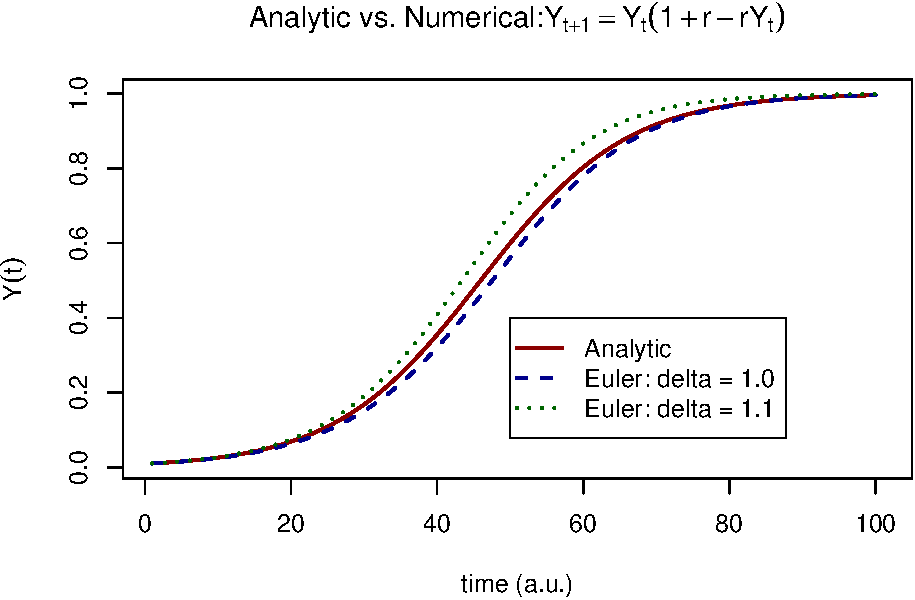
\includegraphics{DCS1617_files/figure-latex/unnamed-chunk-39-1.pdf}

\subsubsection*{Numerical integration}\label{numerical-integration-1}
\addcontentsline{toc}{subsubsection}{Numerical integration}

The Euler setup:

\begin{align}
R_{t+1} &= f_R(R_t,Ft) * \Delta + R_t \\
F_{t+1} &= f_F(R_t,F_t) * \Delta + F_t
\end{align}

With the equations:

\begin{align}
R_{t+1} &=  (a-b*F_t)*R_t * \Delta + R_t \\
\\
F_{t+1} &=  (c*R_t-d)*F_t * \Delta + F_t
\end{align}

\begin{Shaded}
\begin{Highlighting}[]
\CommentTok{# Parameters}
\NormalTok{N  <-}\StringTok{ }\DecValTok{1000}
\NormalTok{a  <-}\StringTok{ }\NormalTok{d <-}\StringTok{ }\DecValTok{1}
\NormalTok{b  <-}\StringTok{ }\NormalTok{c <-}\StringTok{ }\DecValTok{2} 
\NormalTok{R0 <-}\StringTok{ }\NormalTok{F0 <-}\StringTok{ }\FloatTok{0.1}
\NormalTok{R  <-}\StringTok{ }\KeywordTok{as.numeric}\NormalTok{(}\KeywordTok{c}\NormalTok{(R0, }\KeywordTok{rep}\NormalTok{(}\OtherTok{NA}\NormalTok{,N}\DecValTok{-1}\NormalTok{)))}
\NormalTok{F  <-}\StringTok{ }\KeywordTok{as.numeric}\NormalTok{(}\KeywordTok{c}\NormalTok{(F0, }\KeywordTok{rep}\NormalTok{(}\OtherTok{NA}\NormalTok{,N}\DecValTok{-1}\NormalTok{)))}

\CommentTok{# Time constant}
\NormalTok{delta <-}\StringTok{ }\FloatTok{0.01}

\CommentTok{# Numerical integration of the logistic differential equation}
\KeywordTok{l_ply}\NormalTok{(}\KeywordTok{seq_along}\NormalTok{(R), function(t)\{}
    \NormalTok{R[[t}\DecValTok{+1}\NormalTok{]] <<-}\StringTok{ }\NormalTok{(a -}\StringTok{ }\NormalTok{b *}\StringTok{ }\NormalTok{F[t]) *}\StringTok{ }\NormalTok{R[t] *}\StringTok{ }\NormalTok{delta +}\StringTok{ }\NormalTok{R[t] }
    \NormalTok{F[[t}\DecValTok{+1}\NormalTok{]] <<-}\StringTok{ }\NormalTok{(c *}\StringTok{ }\NormalTok{R[t] -}\StringTok{ }\NormalTok{d) *}\StringTok{ }\NormalTok{F[t] *}\StringTok{ }\NormalTok{delta +}\StringTok{ }\NormalTok{F[t] }
    \NormalTok{\})}

\CommentTok{# Note different behaviour when ts() is applied}
\KeywordTok{xyplot}\NormalTok{(}\KeywordTok{cbind}\NormalTok{(}\KeywordTok{ts}\NormalTok{(R),}\KeywordTok{ts}\NormalTok{(F)))}
\end{Highlighting}
\end{Shaded}

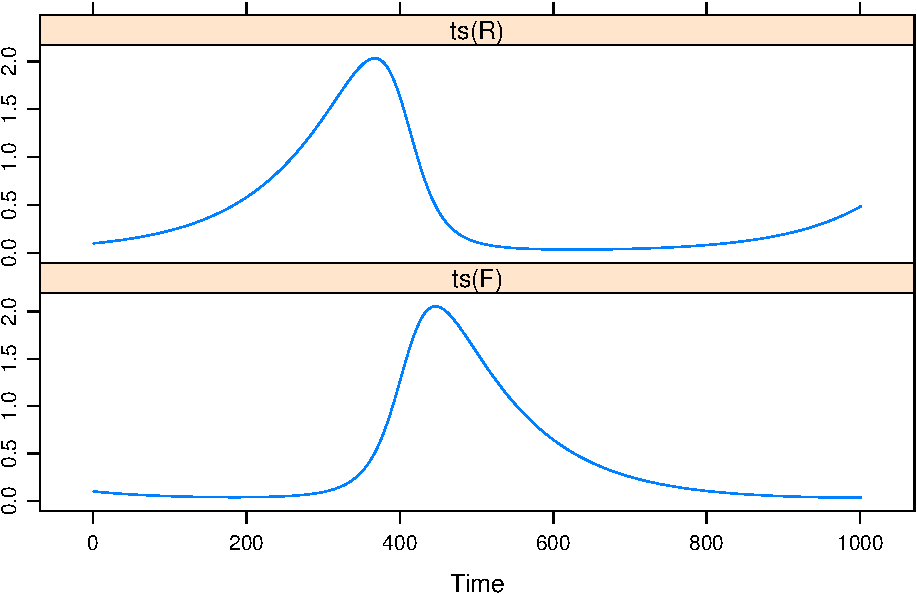
\includegraphics{DCS1617_files/figure-latex/unnamed-chunk-40-1.pdf}

\begin{Shaded}
\begin{Highlighting}[]
\KeywordTok{xyplot}\NormalTok{(R ~}\StringTok{ }\NormalTok{F, }\DataTypeTok{pch =} \DecValTok{16}\NormalTok{)}
\end{Highlighting}
\end{Shaded}

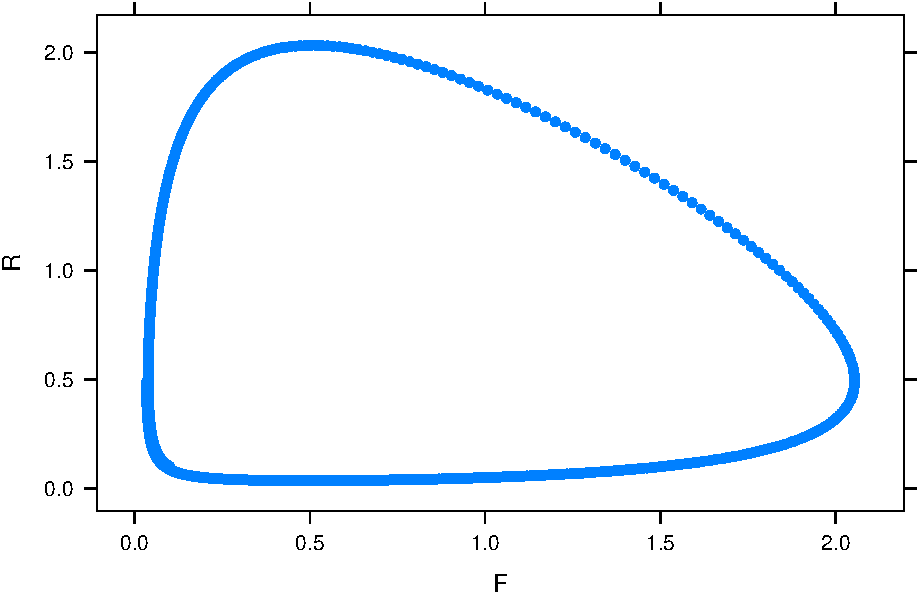
\includegraphics{DCS1617_files/figure-latex/unnamed-chunk-40-2.pdf}

\hypertarget{btasol}{\chapter{\texorpdfstring{\textbf{Basic Timeseries
Analysis}}{Basic Timeseries Analysis}}\label{btasol}}

\section{Nonlinear Growth curves in
SPSS}\label{nonlinear-growth-curves-in-spss}

\protect\hyperlink{bta}{\textbar{} Jump to question \textbar{}}

The solutions are provided as an \texttt{SPSS}
\href{https://raw.githubusercontent.com/FredHasselman/DCS/master/assignmentData/BasicTSA_nonlinreg/GrowthRegression_sol.sps}{syntax
file} file.

Or copy the block below:

\begin{verbatim}
GRAPH
  /LINE(SIMPLE)=VALUE(Yt) BY Time.

* NonLinear Regression.
MODEL PROGRAM  Yzero=0.01 r=0.01 K=0.01.
COMPUTE  PRED_=K*Yzero/(Yzero + (K-Yzero) * EXP(-1*(r * K * Time))).
NLR Yt
  /PRED PRED_
  /SAVE PRED
  /CRITERIA SSCONVERGENCE 1E-8 PCON 1E-8.

GRAPH
  /LINE(MULTIPLE)=VALUE(Yt PRED_) BY Time.

COMPUTE T1=Yt * Time.
COMPUTE T2=Yt * (Time ** 2).
COMPUTE T3=Yt * (Time ** 3).
COMPUTE T4=Yt * (Time ** 4).
EXECUTE.

REGRESSION
  /MISSING LISTWISE
  /STATISTICS COEFF OUTS R ANOVA
  /CRITERIA=PIN(.05) POUT(.10)
  /NOORIGIN 
  /DEPENDENT Yt
  /METHOD=ENTER T1 T2 T3 T4
  /SAVE PRED.


GRAPH
  /LINE(MULTIPLE)=VALUE(Yt PRED_ PRE_1) BY Time.
\end{verbatim}

\begin{itemize}
\tightlist
\item
  The point here is that the polynomial regression appoach is ``just''
  curve fitting \ldots{} adding components until a nice fit is found
  \ldots{} but what does component \(Y_t^4\) represent? A quartic
  subprocess?
\item
  Fitting the solution of the the logistic function will give us
  parameters we can interpret unambiguoulsy: Carrying capacity, growth
  rate, starting value.
\end{itemize}

\hypertarget{pacfsol}{\section{Correlation functions and AR-MA
models}\label{pacfsol}}

\protect\hyperlink{pacfsol}{\textbar{} Jump to question \textbar{}}

The solutions are provided as an \texttt{SPSS}
\href{https://raw.githubusercontent.com/FredHasselman/DCS/master/assignmentData/BasicTSA_arma/Solution_TS_assignment.sps}{syntax
file} file.

Or copy the block below:

\begin{verbatim}
DESCRIPTIVES
  VARIABLES=TS_1 TS_2 TS_3
  /STATISTICS=MEAN STDDEV MIN MAX .

*Sequence Charts .
TSPLOT VARIABLES= TS_1
  /NOLOG
  /FORMAT NOFILL REFERENCE.
TSPLOT VARIABLES= TS_2
  /NOLOG
  /FORMAT NOFILL REFERENCE.
TSPLOT VARIABLES= TS_3
  /NOLOG
  /FORMAT NOFILL REFERENCE.

*ACF and PCF.
ACF
  VARIABLES= TS_1 TS_2 TS_3
  /NOLOG
  /MXAUTO 30
  /SERROR=IND
  /PACF.

* ARIMA with p=5 and q=1.
TSET PRINT=DEFAULT CIN=95 NEWVAR=ALL .
PREDICT THRU END.
ARIMA TS_2
  /MODEL=( 5 0 1)CONSTANT
  /MXITER= 10
  /PAREPS= .001
  /SSQPCT= .001
  /FORECAST= EXACT .

* ARIMA with p=2 and q=1.
TSET PRINT=DEFAULT CIN=95 NEWVAR=ALL .
PREDICT THRU END.
ARIMA TS_2
  /MODEL=( 2 0 1)CONSTANT
  /MXITER= 10
  /PAREPS= .001
  /SSQPCT= .001
  /FORECAST= EXACT .

*Plot Fit.
GRAPH
  /LINE(MULTIPLE)=MEAN(TS_2) MEAN(FIT_2) MEAN(LCL_2) MEAN(UCL_2) BY TIME
  /MISSING=LISTWISE .

*Return plots.

COMPUTE TS_1_lag1 = LAG(TS_1) .
COMPUTE TS_2_lag1 = LAG(TS_2) .
COMPUTE TS_3_lag1 = LAG(TS_3) .
EXECUTE .


IGRAPH /VIEWNAME='Scatterplot' /X1 = VAR(TS_1_lag1) TYPE = SCALE /Y =
  VAR(TS_1) TYPE = SCALE /COORDINATE = VERTICAL  /X1LENGTH=3.0 /YLENGTH=3.0
  /X2LENGTH=3.0 /CHARTLOOK='NONE' /SCATTER COINCIDENT = NONE.
EXE.

IGRAPH /VIEWNAME='Scatterplot' /X1 = VAR(TS_2_lag1) TYPE = SCALE /Y =
  VAR(TS_2) TYPE = SCALE /COORDINATE = VERTICAL  /X1LENGTH=3.0 /YLENGTH=3.0
  /X2LENGTH=3.0 /CHARTLOOK='NONE' /SCATTER COINCIDENT = NONE.
EXE.

IGRAPH /VIEWNAME='Scatterplot' /X1 = VAR(TS_3_lag1) TYPE = SCALE /Y =
  VAR(TS_3) TYPE = SCALE /COORDINATE = VERTICAL  /X1LENGTH=3.0 /YLENGTH=3.0
  /X2LENGTH=3.0 /CHARTLOOK='NONE' /SCATTER COINCIDENT = NONE.
EXE.
\end{verbatim}

\begin{itemize}
\tightlist
\item
  Were you surprised finding out Timeseries 3 is the logisitc map in the
  chaotic regime? It ruly `looks' random (according to PACF).
\end{itemize}

\section{\texorpdfstring{Using \texttt{R} to fit the
solutions}{Using R to fit the solutions}}\label{using-r-to-fit-the-solutions}

There are several packages that can perform nonlinear regression
analysis, the function most resembling the approach used by
\texttt{SPSS} is \texttt{nls} in the default \texttt{stats} package.

The easiest way to do this is to first define your function (i.e., the
solution) and then fit it using starting values for the parameters.

\begin{Shaded}
\begin{Highlighting}[]
\KeywordTok{library}\NormalTok{(rio)}
\NormalTok{df <-}\StringTok{ }\KeywordTok{import}\NormalTok{(}\StringTok{"https://raw.githubusercontent.com/FredHasselman/DCS/master/assignmentData/BasicTSA_nonlinreg/GrowthRegression.sav"}\NormalTok{, }\DataTypeTok{setclass =} \StringTok{"tbl_df"}\NormalTok{)}

\CommentTok{# Logistic growth}
\CommentTok{# Same as SPSS syntax: PRED_=K*Yzero/(Yzero + (K-Yzero) * EXP(-1*(r * K * Time))).}
\NormalTok{log.eq <-}\StringTok{ }\NormalTok{function(Yzero, r, K, Time) \{}
    \NormalTok{K*Yzero/(Yzero +}\StringTok{ }\NormalTok{(K-Yzero) *}\StringTok{ }\KeywordTok{exp}\NormalTok{(-}\DecValTok{1}\NormalTok{*(r *}\StringTok{ }\NormalTok{K *}\StringTok{ }\NormalTok{Time)))}
\NormalTok{\}}
\end{Highlighting}
\end{Shaded}

There is one drawback and you can read about in the help pages:

\begin{quote}
Warning

Do not use nls on artificial ``zero-residual'' data.
\end{quote}

This means, ``do not use it on data generated by a deterministic model
which has no residual error'', which is exactly what the timeseries in
this assignment is, it is the output of the quadratic map in the chaotic
regime.

So, this will give an error:

\begin{Shaded}
\begin{Highlighting}[]
\CommentTok{# Fit this function ... gives an error}
\CommentTok{# The list after 'start' provides the initial values}
\NormalTok{m.log <-}\StringTok{ }\KeywordTok{nls}\NormalTok{(Yt ~}\StringTok{ }\KeywordTok{log.eq}\NormalTok{(Yzero, r, K, Time), }\DataTypeTok{data =} \NormalTok{df, }\DataTypeTok{start =} \KeywordTok{list}\NormalTok{(}\DataTypeTok{Yzero=}\NormalTok{.}\DecValTok{01}\NormalTok{, }\DataTypeTok{r=}\NormalTok{.}\DecValTok{01}\NormalTok{, }\DataTypeTok{K=}\DecValTok{1}\NormalTok{), }\DataTypeTok{trace =} \NormalTok{T)}
\end{Highlighting}
\end{Shaded}

It is possible to fit these ideal data using package
\texttt{minpack.lm}, which contains function \texttt{nlsM}.

\begin{Shaded}
\begin{Highlighting}[]
\KeywordTok{library}\NormalTok{(minpack.lm)}

\NormalTok{m.log <-}\StringTok{ }\KeywordTok{nlsLM}\NormalTok{(Yt ~}\StringTok{ }\KeywordTok{log.eq}\NormalTok{(Yzero, r, K, Time), }\DataTypeTok{data =} \NormalTok{df, }\DataTypeTok{start =} \KeywordTok{list}\NormalTok{(}\DataTypeTok{Yzero =} \NormalTok{.}\DecValTok{01}\NormalTok{, }\DataTypeTok{r=}\NormalTok{.}\DecValTok{01}\NormalTok{, }\DataTypeTok{K=}\FloatTok{0.1}\NormalTok{))}

\KeywordTok{summary}\NormalTok{(m.log)}
\end{Highlighting}
\end{Shaded}

\begin{verbatim}

Formula: Yt ~ log.eq(Yzero, r, K, Time)

Parameters:
       Estimate Std. Error t value Pr(>|t|)    
Yzero 7.055e-03  8.983e-05   78.53   <2e-16 ***
r     1.491e-01  4.170e-04  357.59   <2e-16 ***
K     1.002e+00  4.376e-04 2289.42   <2e-16 ***
---
Signif. codes:  0 '***' 0.001 '**' 0.01 '*' 0.05 '.' 0.1 ' ' 1

Residual standard error: 0.002865 on 97 degrees of freedom

Number of iterations to convergence: 13 
Achieved convergence tolerance: 1.49e-08
\end{verbatim}

In order to look at the model prediction, we use \texttt{predict()}
which is defined for almost all modelfitting functions in \texttt{R}

\begin{Shaded}
\begin{Highlighting}[]
\NormalTok{Ypred <-}\StringTok{ }\KeywordTok{predict}\NormalTok{(m.log)}

\KeywordTok{plot}\NormalTok{(}\KeywordTok{ts}\NormalTok{(df$Yt), }\DataTypeTok{col=}\StringTok{"gray40"}\NormalTok{, }\DataTypeTok{lwd=}\DecValTok{5}\NormalTok{, }\DataTypeTok{ylab =} \NormalTok{(}\StringTok{"Yt | Ypred"}\NormalTok{))}
\KeywordTok{lines}\NormalTok{(Ypred, }\DataTypeTok{col=}\StringTok{"gray80"}\NormalTok{, }\DataTypeTok{lwd=}\DecValTok{2}\NormalTok{, }\DataTypeTok{lty=}\DecValTok{2}\NormalTok{)}
\end{Highlighting}
\end{Shaded}

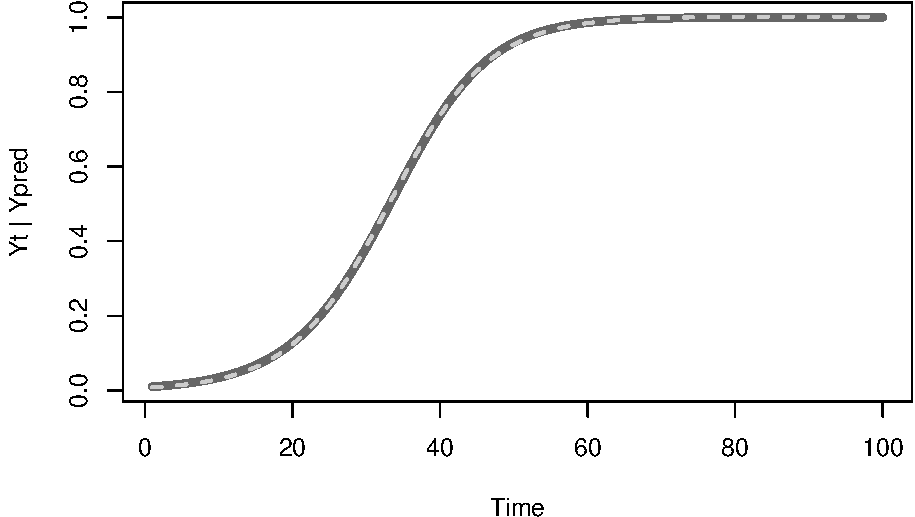
\includegraphics{DCS1617_files/figure-latex/unnamed-chunk-44-1.pdf}

Then we do a polynomial regression using \texttt{lm}:

\begin{Shaded}
\begin{Highlighting}[]
\CommentTok{# Mimic the SPSS syntax}
\KeywordTok{attach}\NormalTok{(df)}
  \NormalTok{df$T1 <-}\StringTok{ }\NormalTok{Yt *}\StringTok{ }\NormalTok{Time}
  \NormalTok{df$T2 <-}\StringTok{ }\NormalTok{Yt *}\StringTok{ }\NormalTok{(Time^}\DecValTok{2}\NormalTok{) }
  \NormalTok{df$T3 <-}\StringTok{ }\NormalTok{Yt *}\StringTok{ }\NormalTok{(Time^}\DecValTok{3}\NormalTok{) }
  \NormalTok{df$T4 <-}\StringTok{ }\NormalTok{Yt *}\StringTok{ }\NormalTok{(Time^}\DecValTok{4}\NormalTok{)}
\KeywordTok{detach}\NormalTok{(df)}

\NormalTok{m.poly <-}\StringTok{ }\KeywordTok{lm}\NormalTok{(Yt ~}\StringTok{ }\NormalTok{T1 +}\StringTok{ }\NormalTok{T2 +}\StringTok{ }\NormalTok{T3 +}\StringTok{ }\NormalTok{T4, }\DataTypeTok{data=}\NormalTok{df)}
\KeywordTok{summary}\NormalTok{(m.poly)}
\end{Highlighting}
\end{Shaded}

\begin{verbatim}

Call:
lm(formula = Yt ~ T1 + T2 + T3 + T4, data = df)

Residuals:
       Min         1Q     Median         3Q        Max 
-0.0117491 -0.0046800 -0.0000683  0.0045719  0.0112732 

Coefficients:
              Estimate Std. Error t value Pr(>|t|)    
(Intercept)  2.113e-02  1.258e-03   16.80   <2e-16 ***
T1           6.366e-02  7.169e-04   88.80   <2e-16 ***
T2          -1.497e-03  3.100e-05  -48.28   <2e-16 ***
T3           1.510e-05  4.425e-07   34.12   <2e-16 ***
T4          -5.529e-08  2.055e-09  -26.90   <2e-16 ***
---
Signif. codes:  0 '***' 0.001 '**' 0.01 '*' 0.05 '.' 0.1 ' ' 1

Residual standard error: 0.005506 on 95 degrees of freedom
Multiple R-squared:  0.9998,    Adjusted R-squared:  0.9998 
F-statistic: 1.264e+05 on 4 and 95 DF,  p-value: < 2.2e-16
\end{verbatim}

Then, predict and plot!

\begin{Shaded}
\begin{Highlighting}[]
\NormalTok{Ypoly <-}\StringTok{ }\KeywordTok{predict}\NormalTok{(m.poly)}

\KeywordTok{plot}\NormalTok{(}\KeywordTok{ts}\NormalTok{(Ypoly), }\DataTypeTok{col=}\StringTok{"blue1"}\NormalTok{, }\DataTypeTok{lwd=}\DecValTok{2}\NormalTok{, }\DataTypeTok{ylab =} \NormalTok{(}\StringTok{"Ypoly (blue) | Ypred (red)"}\NormalTok{))}
\KeywordTok{lines}\NormalTok{(Ypred, }\DataTypeTok{col=}\StringTok{"red1"}\NormalTok{, }\DataTypeTok{lwd=}\DecValTok{2}\NormalTok{)}
\end{Highlighting}
\end{Shaded}

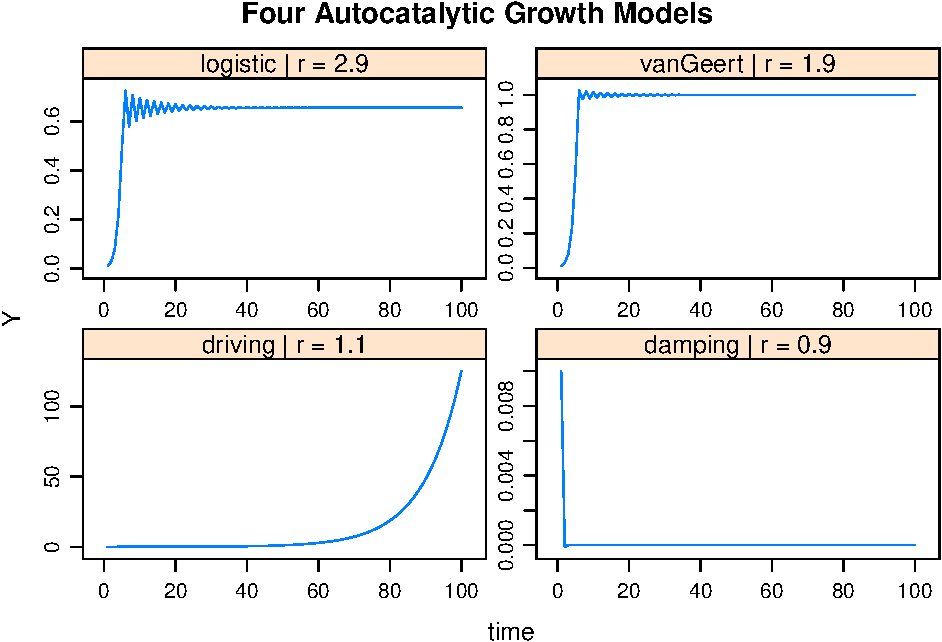
\includegraphics{DCS1617_files/figure-latex/unnamed-chunk-46-1.pdf}

SPSS computes an \(r^2\) value for nonlinear regression models, which
doesn't make a lot of sense if you think about it. Here we van just
compare the residual errors:

\begin{itemize}
\tightlist
\item
  Polynomial regression: \(0.005506\)
\item
  Analytic solution: \(0.002865\)"
\end{itemize}

Slightly less residual error for the analytic solution, using less
parameters to fit the model (3 vs.~5). \textbf{More important:}, the
paramters of the analytic solution have a direct interpretation in terms
of growth processes.

\hypertarget{hrvsol}{\section{Heartbeat dynamics}\label{hrvsol}}

\protect\hyperlink{hrv}{\textbar{} jump to assignment \textbar{}}

\begin{Shaded}
\begin{Highlighting}[]
\KeywordTok{library}\NormalTok{(rio)}
\NormalTok{TS1 <-}\StringTok{ }\NormalTok{rio::}\KeywordTok{import}\NormalTok{(}\StringTok{"https://github.com/FredHasselman/DCS/raw/master/assignmentData/RelativeRoughness/TS1.xlsx"}\NormalTok{, }\DataTypeTok{col_names=}\OtherTok{FALSE}\NormalTok{)}
\NormalTok{TS2 <-}\StringTok{ }\NormalTok{rio::}\KeywordTok{import}\NormalTok{(}\StringTok{"https://github.com/FredHasselman/DCS/raw/master/assignmentData/RelativeRoughness/TS2.xlsx"}\NormalTok{, }\DataTypeTok{col_names=}\OtherTok{FALSE}\NormalTok{)}
\NormalTok{TS3 <-}\StringTok{ }\NormalTok{rio::}\KeywordTok{import}\NormalTok{(}\StringTok{"https://github.com/FredHasselman/DCS/raw/master/assignmentData/RelativeRoughness/TS3.xlsx"}\NormalTok{, }\DataTypeTok{col_names=}\OtherTok{FALSE}\NormalTok{)}
\end{Highlighting}
\end{Shaded}

The Excel files did not have any column names, so let's create them in
the \texttt{data.frame}

\begin{Shaded}
\begin{Highlighting}[]
\KeywordTok{colnames}\NormalTok{(TS1) <-}\StringTok{ "TS1"}
\KeywordTok{colnames}\NormalTok{(TS2) <-}\StringTok{ "TS2"}
\KeywordTok{colnames}\NormalTok{(TS3) <-}\StringTok{ "TS3"}
\end{Highlighting}
\end{Shaded}

\begin{Shaded}
\begin{Highlighting}[]
\CommentTok{# Create a function for RR}
\NormalTok{RR <-}\StringTok{ }\NormalTok{function(ts)\{}
\CommentTok{# lag.max = n gives autocovariance of lags 0 ... n, }
\NormalTok{VAR  <-}\StringTok{ }\KeywordTok{acf}\NormalTok{(ts, }\DataTypeTok{lag.max =} \DecValTok{1}\NormalTok{, }\DataTypeTok{type =} \StringTok{'covariance'}\NormalTok{, }\DataTypeTok{plot=}\OtherTok{FALSE}\NormalTok{)}
\CommentTok{# RR formula}
\NormalTok{RelR   <-}\StringTok{ }\DecValTok{2}\NormalTok{*(}\DecValTok{1}\NormalTok{-VAR$acf[}\DecValTok{2}\NormalTok{] /}\StringTok{ }\NormalTok{VAR$acf[}\DecValTok{1}\NormalTok{])}
\CommentTok{# Add some attributes to the output}
\KeywordTok{attributes}\NormalTok{(RelR) <-}\StringTok{ }\KeywordTok{list}\NormalTok{(}\DataTypeTok{localAutoCoVariance =} \NormalTok{VAR$acf[}\DecValTok{2}\NormalTok{], }\DataTypeTok{globalAutoCoVariance =} \NormalTok{VAR$acf[}\DecValTok{1}\NormalTok{]) }
\KeywordTok{return}\NormalTok{(RelR)}
\NormalTok{\}}

\CommentTok{# Look at the results}
\NormalTok{for(ts in }\KeywordTok{list}\NormalTok{(TS1,TS2,TS3))\{}
  \NormalTok{relR <-}\StringTok{ }\KeywordTok{RR}\NormalTok{(ts[,}\DecValTok{1}\NormalTok{])}
  \KeywordTok{cat}\NormalTok{(}\KeywordTok{paste0}\NormalTok{(}\KeywordTok{colnames}\NormalTok{(ts),}\StringTok{": RR = "}\NormalTok{,}\KeywordTok{round}\NormalTok{(relR,}\DataTypeTok{digits=}\DecValTok{3}\NormalTok{), }\StringTok{" = 2*(1-"}\NormalTok{,}
         \KeywordTok{round}\NormalTok{(}\KeywordTok{attributes}\NormalTok{(relR)$localAutoCoVariance, }\DataTypeTok{digits =} \DecValTok{4}\NormalTok{),}\StringTok{"/"}\NormalTok{,}
         \KeywordTok{round}\NormalTok{(}\KeywordTok{attributes}\NormalTok{(relR)$globalAutoCoVariance,}\DataTypeTok{digits =} \DecValTok{4}\NormalTok{),}\StringTok{")}\CharTok{\textbackslash{}n}\StringTok{"}\NormalTok{))}
  \NormalTok{\}}
\end{Highlighting}
\end{Shaded}

\begin{verbatim}
TS1: RR = 0.485 = 2*(1-0.0016/0.0021)
TS2: RR = 0.118 = 2*(1-0.0018/0.0019)
TS3: RR = 2.052 = 2*(1--1e-04/0.002)
\end{verbatim}

Use Figure \ref{fig:RRf3} to lookup which value of \(RR\) corresponds to
which type of noise:

\textbf{TS1}: Pink noise \textbf{TS2}: Brownian noise \textbf{TS3}:
White noise

\subsection{Randomise}\label{randomise}

To randomize the data you may use the function \texttt{sample} (which is
easier than \texttt{randperm})

\begin{Shaded}
\begin{Highlighting}[]
\KeywordTok{library}\NormalTok{(pracma)}
\CommentTok{# randperm()}
\NormalTok{TS1Random <-}\StringTok{ }\NormalTok{TS1$TS1[}\KeywordTok{randperm}\NormalTok{(}\KeywordTok{length}\NormalTok{(TS1$TS1))]}

\CommentTok{# sample()}
\NormalTok{TS1Random <-}\StringTok{ }\KeywordTok{sample}\NormalTok{(TS1$TS1, }\KeywordTok{length}\NormalTok{(TS1$TS1))}

\KeywordTok{plot.ts}\NormalTok{(TS1Random)}
\KeywordTok{lines}\NormalTok{(}\KeywordTok{ts}\NormalTok{(TS1$TS1),}\DataTypeTok{col=}\StringTok{"red3"}\NormalTok{)}
\end{Highlighting}
\end{Shaded}

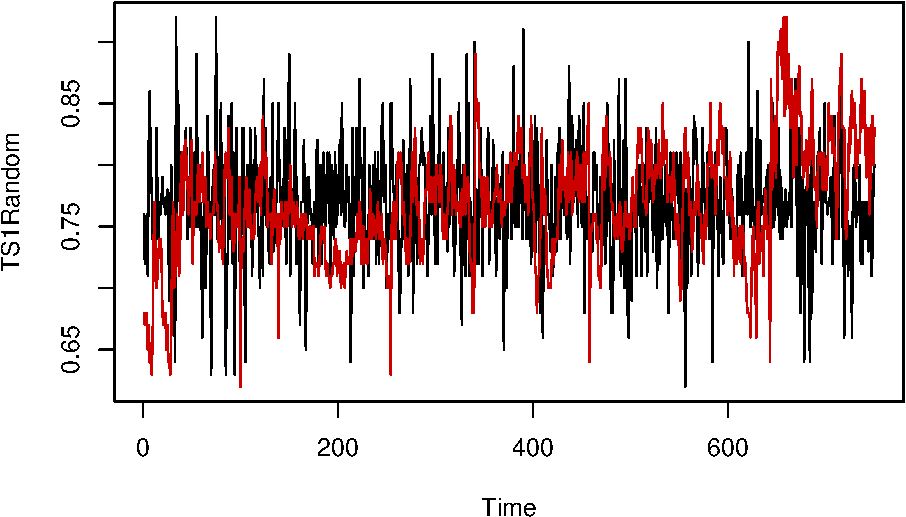
\includegraphics{DCS1617_files/figure-latex/unnamed-chunk-50-1.pdf}

If you repeat this for TS2 and TS3 and compute the Relative Roughness of
each randomized time series, the outcomes should be around 2, white
noise! This makes sense, you destroyed all the correlations in the data
by removing the temporal order with which values were observed.

\subsection{Integrate}\label{integrate}

Normalize the white noise time series

\begin{Shaded}
\begin{Highlighting}[]
\NormalTok{TS3Norm <-}\StringTok{ }\KeywordTok{scale}\NormalTok{(TS3$TS3)}
\end{Highlighting}
\end{Shaded}

Now integrate it, which just means, `take the cumulative sum'.

\begin{Shaded}
\begin{Highlighting}[]
\NormalTok{TS3Int <-}\StringTok{ }\KeywordTok{cumsum}\NormalTok{(TS3Norm)}
\KeywordTok{plot.ts}\NormalTok{(TS3Int)}
\KeywordTok{lines}\NormalTok{(}\KeywordTok{ts}\NormalTok{(TS3Norm),}\DataTypeTok{col=}\StringTok{"red3"}\NormalTok{)}
\end{Highlighting}
\end{Shaded}

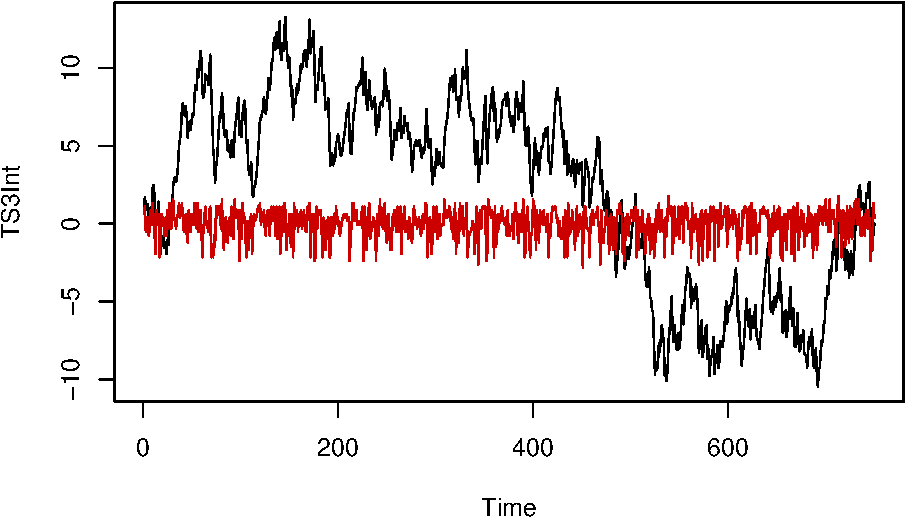
\includegraphics{DCS1617_files/figure-latex/unnamed-chunk-52-1.pdf}

If you compute the Relative Roughness of the integrated time series, the
outcome should be close to 0, Brownian noise.

\begin{Shaded}
\begin{Highlighting}[]
\KeywordTok{RR}\NormalTok{(TS3Int)}
\end{Highlighting}
\end{Shaded}

\begin{verbatim}
[1] 0.02783704
attr(,"localAutoCoVariance")
[1] 35.69734
attr(,"globalAutoCoVariance")
[1] 36.2012
\end{verbatim}

\chapter{\texorpdfstring{\textbf{Fluctuation and Disperion analyses
I}}{Fluctuation and Disperion analyses I}}\label{fda1sol}

\hypertarget{psdsol}{\section{Assignment: The Spectral
Slope}\label{psdsol}}

\protect\hyperlink{psd}{\textbar{} jump to assignment \textbar{}}

\BeginKnitrBlock{rmdimportant}
First, load the data and source the function library.
\EndKnitrBlock{rmdimportant}

\subsection{\texorpdfstring{Example of using \texttt{-\/-ply}
functions}{Example of using -\/-ply functions}}\label{example-of-using---ply-functions}

Let's try to use as few commands as possible to analyse all three
timeseries. The easiest way to do this is to use the so-called
\texttt{apply} family of functions.

These functions pass the contents of a \texttt{list} object to a
function. Suppose we need to calculate the means of column variables in
40 different SPSS \texttt{.sav} files stored in the folder \texttt{DAT}.
With the \texttt{rio} package loaded we can execute the following
commands:

\begin{Shaded}
\begin{Highlighting}[]
\NormalTok{data <-}\StringTok{ }\KeywordTok{lapply}\NormalTok{(}\KeywordTok{dir}\NormalTok{(}\StringTok{"/DAT/"}\NormalTok{,}\DataTypeTok{pattern=}\StringTok{".sav$"}\NormalTok{),import)       }
\NormalTok{out  <-}\StringTok{ }\KeywordTok{sapply}\NormalTok{(data,colMeans)}
\end{Highlighting}
\end{Shaded}

The first command \emph{applies} \texttt{import} to all files with a
\texttt{.sav} extension found in the folder \texttt{/DAT}. It creates a
dataframe for each file which are all stored as elements of the list
object \texttt{data}. The second line applies the function
\texttt{colMeans} to each element of \texttt{data} and puts the combined
results in a matrix with the dataset ID as columns (1-40), dataset
variables as rows and the calculated column means as cells.

\texttt{R} comes with several \texttt{apply} functions installed, but an
easier interface is provided by package \texttt{plyr}. When
\texttt{plyr} is loaded you can use functions of the type \texttt{XYply}
where \texttt{X} denotes the first letter of the input structure and
\texttt{Y} the ouput structure: \texttt{l} for \texttt{list}, \texttt{d}
\texttt{for\ \textquotesingle{}data.frame}, \texttt{a} for
\texttt{array}. So, \texttt{laply()} expects a listobject as input and
will try to create an array as outout. There is also a special symbol
for \texttt{Y}, the underscore \texttt{\_} if no output is expected,
e.g.~when plotting, \texttt{l\_ply}.

\subsection{Data preparation}\label{data-preparation}

Let's prepare these series for spectral analysis.

\begin{Shaded}
\begin{Highlighting}[]
\KeywordTok{library}\NormalTok{(plyr)}
\NormalTok{TSlist <-}\StringTok{ }\KeywordTok{list}\NormalTok{(}\DataTypeTok{TS1=}\NormalTok{TS1$TS1,}\DataTypeTok{TS2=}\NormalTok{TS2$TS2,}\DataTypeTok{TS3=}\NormalTok{TS3$TS3)}

\CommentTok{# Plot raw}
\KeywordTok{l_ply}\NormalTok{(TSlist, plot.ts)}
\end{Highlighting}
\end{Shaded}

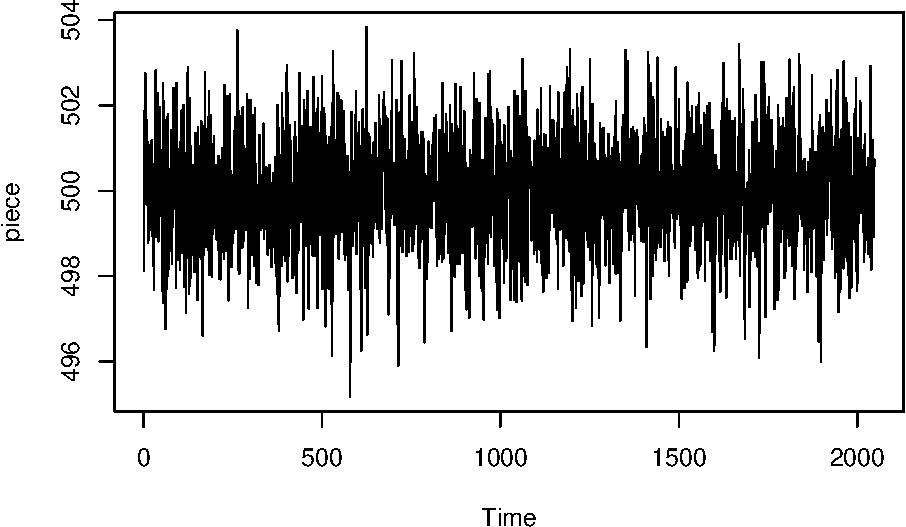
\includegraphics{DCS1617_files/figure-latex/unnamed-chunk-56-1.pdf}
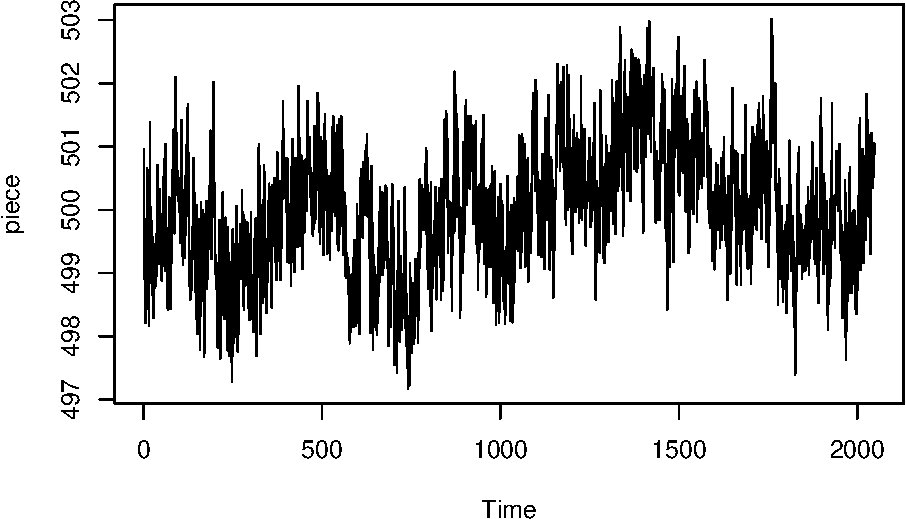
\includegraphics{DCS1617_files/figure-latex/unnamed-chunk-56-2.pdf}
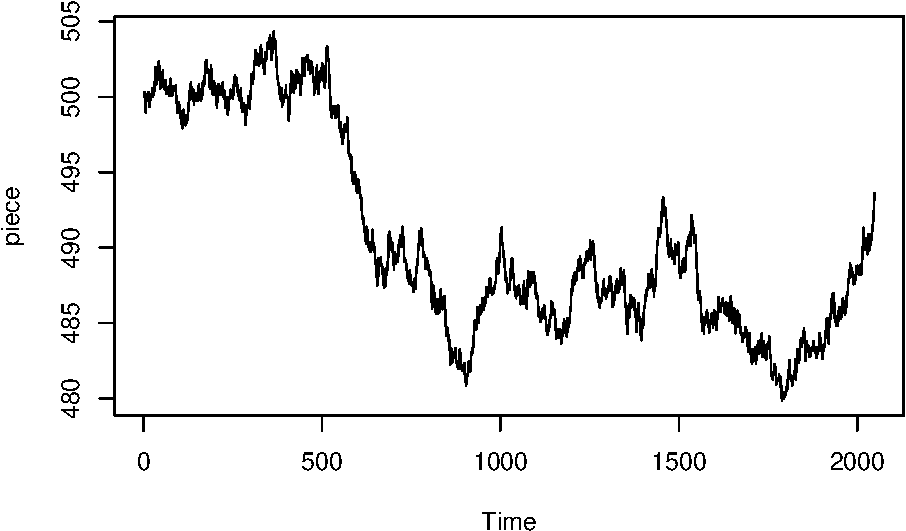
\includegraphics{DCS1617_files/figure-latex/unnamed-chunk-56-3.pdf}

\begin{Shaded}
\begin{Highlighting}[]
\CommentTok{# Normalise}
\NormalTok{TSlist.n <-}\StringTok{ }\KeywordTok{llply}\NormalTok{(TSlist,scale)}

\CommentTok{# Plot normalised}
\KeywordTok{l_ply}\NormalTok{(TSlist.n, plot.ts)}
\end{Highlighting}
\end{Shaded}

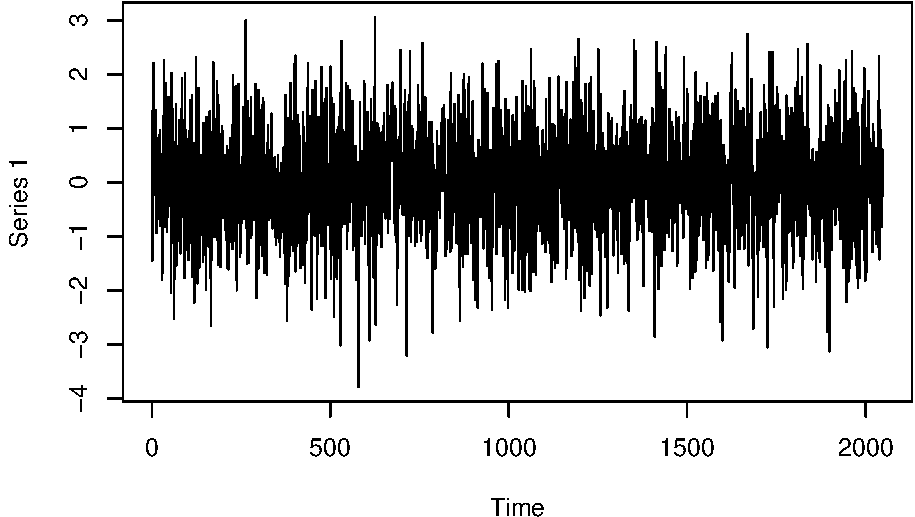
\includegraphics{DCS1617_files/figure-latex/unnamed-chunk-56-4.pdf}
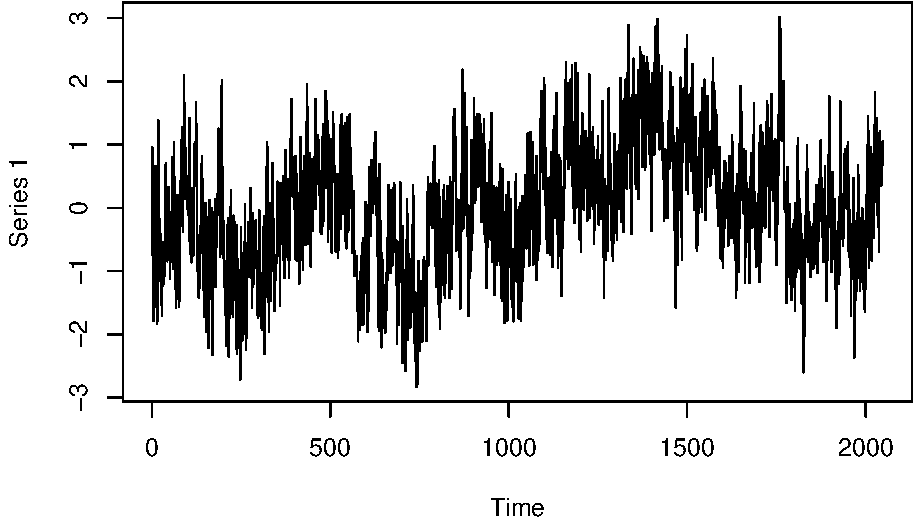
\includegraphics{DCS1617_files/figure-latex/unnamed-chunk-56-5.pdf}
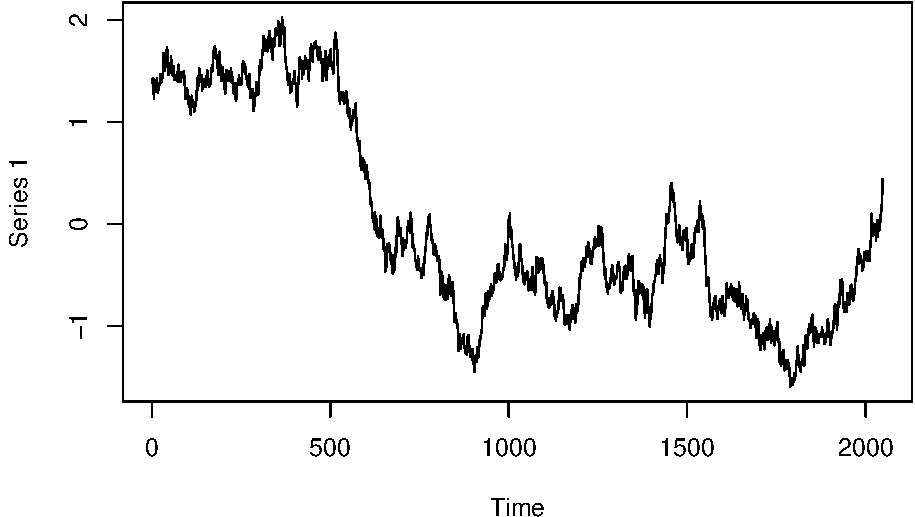
\includegraphics{DCS1617_files/figure-latex/unnamed-chunk-56-6.pdf}

\begin{Shaded}
\begin{Highlighting}[]
\CommentTok{# Detrend}
\NormalTok{TSlist.nd <-}\StringTok{ }\KeywordTok{llply}\NormalTok{(TSlist.n, detrend)}

\CommentTok{# Plot normalised, detrended}
\KeywordTok{l_ply}\NormalTok{(TSlist.nd, plot.ts)}
\end{Highlighting}
\end{Shaded}

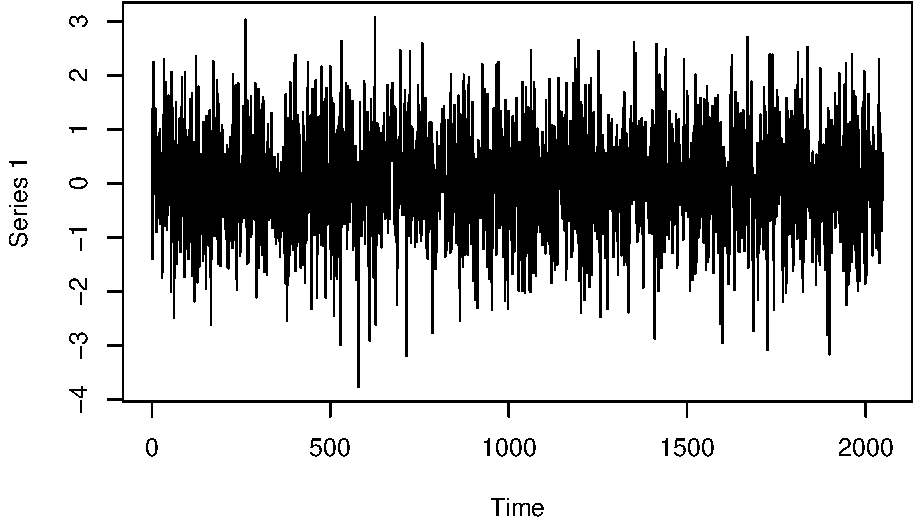
\includegraphics{DCS1617_files/figure-latex/unnamed-chunk-56-7.pdf}
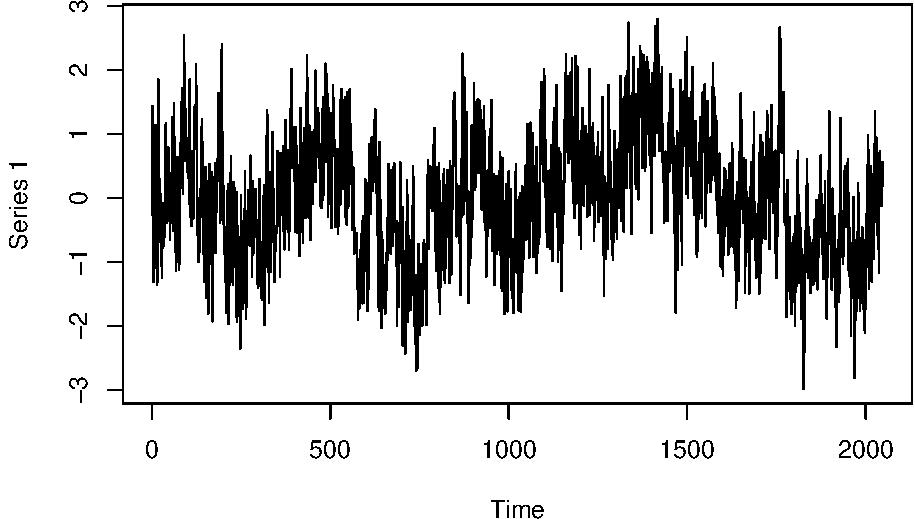
\includegraphics{DCS1617_files/figure-latex/unnamed-chunk-56-8.pdf}
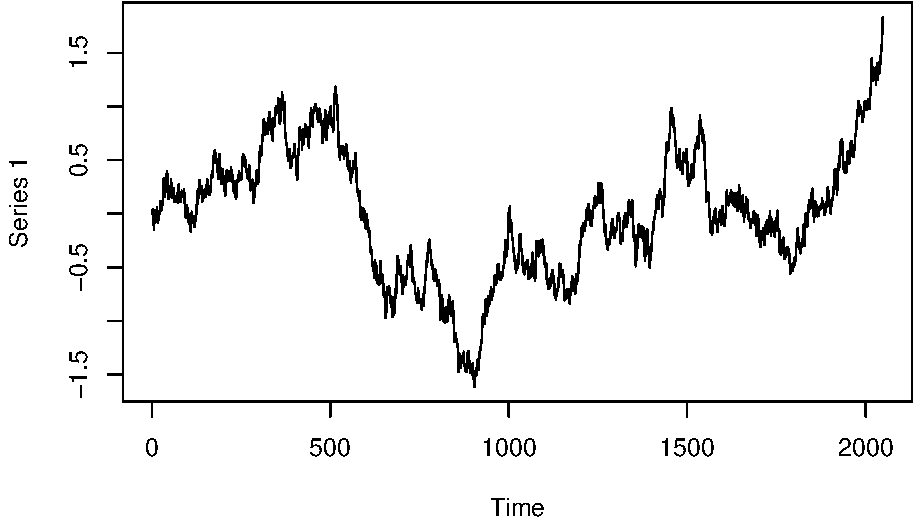
\includegraphics{DCS1617_files/figure-latex/unnamed-chunk-56-9.pdf}

\subsection{Time-series length}\label{time-series-length}

Another preparation concerns checking wether the length of the series is
a power of 2 (or 10). This is necessary for the Fourier transfrom to run
smoothly. The code below uses \texttt{log2} and \texttt{nextpow2} to
figure out whether the data length is ok.

What is different from previous uses of the \texttt{XYply} functions is
that we now customise the function we want to execute. The input is
still a list object, each element of the list is passed as a variable
\texttt{ts} to a so-called \texttt{anonymous} function, a function just
denoted as \texttt{function(ts)}. The function returns a data.frame with
columns \texttt{pow2}, the current power of 2 and \texttt{nextpow2} (a
function of \texttt{pracma}) the next power of 2.

The \texttt{XYply} functions will add an \texttt{.id} variable to the
output if the input is a list with named fields. Although we create 3
data frames of one row, the \texttt{d} in \texttt{ldply} indicates these
frames have to be merged if possible.

\begin{Shaded}
\begin{Highlighting}[]
\KeywordTok{ldply}\NormalTok{(TSlist.nd, function(ts) }\KeywordTok{data.frame}\NormalTok{(}\DataTypeTok{pow2 =} \KeywordTok{log2}\NormalTok{(}\KeywordTok{length}\NormalTok{(ts)), }\DataTypeTok{nextpow2 =} \KeywordTok{nextpow2}\NormalTok{(}\KeywordTok{length}\NormalTok{(ts))))}
\end{Highlighting}
\end{Shaded}

\begin{verbatim}
  .id pow2 nextpow2
1 TS1   11       11
2 TS2   11       11
3 TS3   11       11
\end{verbatim}

\begin{itemize}
\tightlist
\item
  In this case we don't have to take any action, \(2048\) is a power of
  2.
\item
  Actions that could be taken are: removing datapoints from the front of
  the series, or, padding the series with zeroes.
\end{itemize}

\subsection{\texorpdfstring{The \texttt{fd.psd}
function}{The fd.psd function}}\label{the-fd.psd-function}

The function created for spectral analysis \texttt{fd.psd()} will
perform normalisation and detrending by default. It also returns
information about the power spectrum and log-log fit. It's good to know
about the default settings of a function, and the return values. The
best place to look for them is usually the \texttt{help} documentation,
or the \texttt{vignettes} that come with a package.

If you select a function in \texttt{Rstudio} and press \texttt{F1}
you'll get the help page, If you press \texttt{F2} can have a look at
the code (if it is \texttt{exported}), or, you can call the function
without parentheses \texttt{fd.psd} and the code will be printed to the
Console.

You can also hover the cursor after you typed the name of the function
to reveal the arguments and defaults:

Another way to get this info is to use the function \texttt{formals()}

\begin{Shaded}
\begin{Highlighting}[]
\KeywordTok{formals}\NormalTok{(fd.psd)}
\end{Highlighting}
\end{Shaded}

\begin{verbatim}
$y


$fs
NULL

$normalize
[1] TRUE

$dtrend
[1] TRUE

$plot
[1] FALSE
\end{verbatim}

Now we know this function has arguments \texttt{normalize} and
\texttt{dtrend} set to \texttt{TRUE}, and \texttt{plot} set to
\texttt{FALSE}. We could feed the fuction the raw data, or feed it our
normalised, detrended, data and change the defaults. In the
\texttt{XYply} functions, you can just add function arguments after the
function name.

\begin{Shaded}
\begin{Highlighting}[]
\CommentTok{# Analyse}
\NormalTok{outPSD <-}\StringTok{ }\KeywordTok{llply}\NormalTok{(TSlist.nd, fd.psd, }\DataTypeTok{normalize =} \OtherTok{FALSE}\NormalTok{, }\DataTypeTok{dtrend =} \OtherTok{FALSE}\NormalTok{, }\DataTypeTok{plot=}\OtherTok{TRUE}\NormalTok{)}
\end{Highlighting}
\end{Shaded}

\begin{verbatim}


fd.psd: Sample rate was set to 1.
\end{verbatim}


\includegraphics{DCS1617_files/figure-latex/unnamed-chunk-60-1.pdf}
\includegraphics{DCS1617_files/figure-latex/unnamed-chunk-60-2.pdf}

\begin{verbatim}


fd.psd: Sample rate was set to 1.
\end{verbatim}

\includegraphics{DCS1617_files/figure-latex/unnamed-chunk-60-3.pdf}
\includegraphics{DCS1617_files/figure-latex/unnamed-chunk-60-4.pdf}

\begin{verbatim}


fd.psd: Sample rate was set to 1.
\end{verbatim}

\includegraphics{DCS1617_files/figure-latex/unnamed-chunk-60-5.pdf}
\includegraphics{DCS1617_files/figure-latex/unnamed-chunk-60-6.pdf}

\chapter{\texorpdfstring{\textbf{Fluctuation and Disperion analyses
II}}{Fluctuation and Disperion analyses II}}\label{fda1so2}

There were no assignments for this Lecture.

\chapter{\texorpdfstring{\textbf{Phase Space Reconstruction and
Recurrence Quantification Analysis
(RQA)}}{Phase Space Reconstruction and Recurrence Quantification Analysis (RQA)}}\label{RQAsol}

\chapter{\texorpdfstring{\textbf{Categorical and Cross-RQA
(CRQA)}}{Categorical and Cross-RQA (CRQA)}}\label{CRQAsol}

\chapter{\texorpdfstring{\textbf{The Cusp Catasrophe Model \& Warning
Signs}}{The Cusp Catasrophe Model \& Warning Signs}}\label{cuspsol}

\chapter{\texorpdfstring{\textbf{Complex
Networks}}{Complex Networks}}\label{netssol}

\chapter*{\texorpdfstring{\textbf{Bibliography}}{Bibliography}}\label{bibliography}
\addcontentsline{toc}{chapter}{\textbf{Bibliography}}

\bibliography{packages.bib,book.bib}


\end{document}
